%dica: use a opção oneside se houver um limite (e.g., 20) de páginas
\documentclass[embeddedlogo, nohidelinks, arial]{ufsc-thesis-rn46-2019}

\usepackage[T1]{fontenc} % fontes
%\usepackage[utf8]{inputenc} % UTF-8
\usepackage{pdfpages} % Inclui PDF externo (ficha catalográfica)
\usepackage{comment}
\usepackage{tikz}
\usepackage{tikzscale}
\usepackage{tikz-cd}
\usetikzlibrary{backgrounds, positioning, fit}
\usepackage{url}

% Para tabelas
\usepackage{siunitx} % Para alinhamento numérico
\usepackage{graphicx} % Para \resizebox
\usepackage{array} % Para ajustes em colunas de tabelas

% Diagrama de sequências
\usepackage{pgf-umlsd}

\usepackage{silence}

% Suprimir avisos específicos sobre sobrescrita de comandos
\WarningFilter{glossaries}{Overriding \printglossary}
\WarningFilter{glossaries}{Overriding `theglossary' environment}

% Todo notes
\usepackage[colorinlistoftodos]{todonotes}

% Para código de JSON
% \usepackage{bera}% optional: just to have a nice mono-spaced font
\usepackage{listings}
\renewcommand{\lstlistingname}{Algoritmo}
\usepackage{xcolor}

% Mudar o esilo do enumerate
\usepackage{enumitem}

\usepackage{subcaption}

\usepackage{nomencl}
\makenomenclature

\usepackage{courier} 


\usepackage{amsthm}
\usepackage{amssymb}
% EXTRACT FROM UFSC THESISCommonly used in definitions, conditions, problems and examples.
\theoremstyle{definition}
\newtheorem{definicao}{Defini\c{c}\~ao}[chapter]
\newtheorem{exemplo}{Exemplo}[section]
\newtheorem{exercicio}{Exerc\'icio}[section]
\newtheorem{condicao}{Condi\c{c}\~ao}[chapter]

\newtheorem{axioma}{Axioma}[chapter]
\newtheorem{postulado}{Postulado}[chapter]
\newtheorem{teorema}{Teorema}[chapter]
\newtheorem{conjectura}{Conjectura}[chapter]
\newtheorem{corolario}[teorema]{Corol\'ario}
\newtheorem{lema}[teorema]{Lema}
\newtheorem{proposicao}[teorema]{Proposi\c{c}\~ao}




\hypersetup{
    colorlinks=true,     % Ativa a coloração dos links
    linkcolor=black,      % Define a cor dos links internos (sumário, referências cruzadas)
    urlcolor=black,       % Define a cor dos links de URLs
    citecolor=blue,       % Define a cor das citações
    filecolor=black       % Define a cor dos links para arquivos
}

\usepackage[%
%xindy={language=portuguese}, %para usar o xindy ao invés do makeindex
subentrycounter,
seeautonumberlist,
nonumberlist,
nogroupskip,
shortcuts,   % criação de atalhos
acronym,  % criação de acrônimos  	
translate=babel, % Faz o papel de \providetranslation
nopostdot,  % Não é colocado ponto ao final da entrada
automake
]{glossaries}


\renewcommand{\glossarypreamble}{\vspace{-0.2cm}}  % Retira o espaço proviniente do estilo

% Criação de estilo

\newglossarystyle{mylong1}{% modificado de https://tex.stackexchange.com/a/166209/151962
	\setglossarystyle{long}%
	\renewenvironment{theglossary}%
	{\begin{longtable}[l]{@{}p{\dimexpr 2.5cm-\tabcolsep}p{0.78\hsize}}}% <-- change the value here
		{\end{longtable}}%
}



% Só um pequeno récuo em relação ao primeiro
\newglossarystyle{mylong2}{% modificado de https://tex.stackexchange.com/a/166209/151962
	\setglossarystyle{long}%
	\renewenvironment{theglossary}%
	{\begin{longtable}[l]{@{}p{\dimexpr 2.0cm-\tabcolsep}p{0.86\hsize}}}% <-- change the value here
		{\end{longtable}}%
}



% Criando o comando sigla. Cria a descrição da sigla e a sigla entre parênteses 
% #1 é o atalho da sigla e a sigla. #2 é a descrição 
\newcommand{\sigla}[2]{\newacronym{#1}{#1}{#2}\acrfull{#1}}

% Só dá entrada na lista. Ainda não funciona com o limarka
\newcommand{\siglalista}[2]{\newacronym{#1}{#1}{#2}}  


\newglossary{simbolos}{simbolos}{sbl}{simbolos}

% Criando o comando simbolo. Imprime o símbolo e sua descrição só é mostrada na lista
% #1 é o atalho. #2 é símbolo. #3 descrição 
\newcommand{\simbolo}[3]{\newglossaryentry{#1}{%
						type=simbolos, 
						name=#2, 
						description=#3,
						sort=def}\gls{#1}}

% Só dá entrada na lista. Ainda não funciona com o limarka
\newcommand{\simbololista}[3]{\newglossaryentry{#1}{%
							type=simbolos, 
							name=#2, 
							description=#3,
							sort=def}}

% 
\newcommand{\imprimirlistadesiglas}{%
	    \pdfbookmark[0]{\listadesiglasname}{acn}	
		\printacronyms[%
				style=mylong1,
				title={Lista de Siglas}  % A lista de siglas ainda fica com um espaço a mais
			  ]
		\cleardoublepage
}

\newcommand{\imprimirlistadesimbolos}{%
   	\pdfbookmark[0]{\listadesimbolosname}{sbl}					
	\printglossary[%
			type=simbolos,
			title={\listadesimbolosname }, 
			style=mylong2
			]

	\cleardoublepage
}


\newcommand{\imprimirglossario}{
    \cleardoublepage
   	\pdfbookmark[0]{\glossaryname}{glo}					
	\printglossary[title={\glossaryname}]
}


\makeglossaries


%%%%%%%%%%%%%%%%%%%%%%%%%%%%%%%%%%%%%%%%%%%%%%%%%%%%%%%%%%%%%%%%%%%%
%%% Configurações da classe (dados do trabalho)                  %%%
%%%%%%%%%%%%%%%%%%%%%%%%%%%%%%%%%%%%%%%%%%%%%%%%%%%%%%%%%%%%%%%%%%%%

% Preâmbulo
\titulo{Protocolo para Negociação de Atributos e Ambiente de Execução na Identidade Fiduciária e Análise Formal de Segurança}
\autor{Victor do Valle Cunha}

% Importante! Para documentos em inglês, não use today, digite a data em
% pt_BR, como deve aparecer na folha de certificação.
\data{13 de Dezembro de 2024}
\instituicao{Universidade Federal de Santa Catarina}
\centro{Centro Tecnológico}
\programa{Programa de Pós-Graduação em Ciência da Computação}
\tcc
\departamento{Departamento de Informática e Estatística}
\curso{Ciência da Computação}
\titulode{Bacharel em Ciência da Computação}
\local{Florianópolis} % Apenas cidade! Sem estado
% template da BU usa doutor/mestre em minúsculo, Bacharel/Licenciado em Title case.

%%% Atenção! No caso de TCC, além de usar \tcc, outros comandos devem ser fornecidos:
%%%
% \tcc
% \departamento{Departamento de Informática e Estatística}
% \curso{Ciência da Computação}
% \titulode{Bacharel em Ciência da Computação}
% %% Para TCCs, orientadores e coorientadores podem ser externos, logo a
% %% BU exige que sua afiliação seja explicitada. Por padrão, assume-se
% %% UFSC. Você pode alterar a afiliação com os comandos abaixo:
% \afiliacaoorientador{Universidade Federal de Santa Catarina}
% \afiliacaocoorientador{Universidade Federal da Terra de Ninguém}

% Orientador, coorientador, membros da banca e coordenador
% As regras da BU agora exigem que Dr. apareça **depois** do nome
% Dica: para gerar Profᵃ. use Prof\textsuperscript{a}.
% Dica 2: para feminino use \orientadora e \coorientadora
\orientador{Prof. Frederico Schardong, Dr.}
\coorientador{Prof. Ricardo Custódio, Dr.}
\membrobanca{Maurício de Vasconcelos Barros}{Universidade Federal de Santa Catarina}
\membrobanca{Brendon Vicente Rocha Silva}{Universidade Federal de Santa Catarina}

% Dica: se feminino, \coordenadora
\coordenador{Prof. Márcio Bastos Castro, Dr}

\begin{document}

%%%%%%%%%%%%%%%%%%%%%%%%%%%%%%%%%%%%%%%%%%%%%%%%%%%%%%%%%%%%%%%%%%%%
%%% Principais elementos pré-textuais                            %%%
%%%%%%%%%%%%%%%%%%%%%%%%%%%%%%%%%%%%%%%%%%%%%%%%%%%%%%%%%%%%%%%%%%%%

% Inicia parte pré-textual do documento capa, folha de rosto, folha de
% aprovação, aprovação, resumo, lista de tabelas, lista de figuras, etc.
\pretextual%
\imprimircapa%
\imprimirfolhaderosto*
\protect\incluirfichacatalografica{ficha.pdf}
\imprimirfolhadecertificacao

\begin{dedicatoria}
À minha mãe e à minha namorada.
\end{dedicatoria}

\begin{agradecimentos}
  Concluir esta monografia não teria sido possível sem o apoio daqueles que estiveram ao meu lado ao longo de toda a jornada. Agradeço, primeiramente, aos amigos que tive a sorte de conhecer durante esse período – Cris, João, Léo, Luan, Dudu e Caz –, com quem compartilhei momentos de aprendizado, companheirismo e incentivo mútuo. Um agradecimento especial vai para Dani, que me apoiou em momentos difíceis e me ofereceu forças quando mais precisei. Aos amigos de longa data, Bia, Rondon, Barcelos e Henrique, agradeço pela confiança e pelo incentivo constante, por nunca terem desistido de mim e por me inspirarem a seguir em frente, independentemente dos desafios.

  Também expresso minha profunda gratidão aos meus familiares – minha tia e meu irmão, que sempre foi um exemplo de dedicação e persistência. À minha namorada, Maria, que esteve ao meu lado de maneira incondicional, agradeço pelo amor, paciência e pelo encorajamento constantes, fundamentais para enfrentar todos os momentos difíceis. Por fim, agradeço especialmente à minha mãe, cujo esforço e comprometimento inabaláveis permitiram que seus filhos alcançassem o sonho da formação acadêmica.
\end{agradecimentos}

\begin{epigrafe}
\textit{"Parabéns mamãe, seu projeto de homem feliz deu certo"} \\ Leandro Roque
\end{epigrafe}


\begin{resumo}[Resumo]
O modelo de Identidade Fiduciária representa uma abordagem inovadora para o desenvolvimento de sistemas de identificação, com foco em solucionar dois desafios centrais dos modelos convencionais: a usabilidade e a proteção da privacidade dos dados do usuário. A inclusão de um novo ator, responsável por atender a essas demandas, permite a definição de propriedades que facilitam o alcance dessas metas. No entanto, a definição dessas propriedades, por si só, é insuficiente. Para que sejam aplicadas de maneira eficaz, é imprescindível contar com protocolos de comunicação seguros entre as três entidades envolvidas no processo de autenticação do usuário: o Emissor, o Fiduciário e o Verificador. Além disso, é essencial que esses protocolos incluam propriedades de segurança específicas, capazes de validá-los em diferentes cenários de uso.
Diante dessas considerações, este trabalho de conclusão de curso adapta e expande o protocolo OpendID para Apresentações Verficáveis (\acs{OIDC4VP}) para o contexto deste novo modelo de identidade, possibilitando a negociação de dados sensíveis no processo de autenticação e a manipulação desses dados em um ambiente de confiança para o usuário. Dessa forma, busca-se uma experiência mais fluida, em que o usuário não precise interagir constantemente com formulários de autorização, mas que ainda preserve as propriedades de segurança essenciais para o cenário proposto.

  % Atenção! a BU exige separação através de ponto (.). Ela recomanda de 3 a 5 keywords
  \vspace{\baselineskip} 
  \textbf{Palavras-chave:} Identidade Eletrônica.  Identidade Digital. Gestão de Identidade. Identidade Autossoberana. Identidade Fiduciária.

\end{resumo}


    % \begin{resumo}[Resumo Estendido]
    
    %   \section*{Objetivos}
    %     Desenvolver um protocolo de comunicação para um novo modelo de identidade eletrônica, descrevendo aspectos sintáticos e semânticos das mensagens trocadas entre a entidade fiduciária e o provedor de serviços, revisando as principais técnicas de Prova de Zero-Conhecimento para geração de Apresentações e selecionando as melhores alternativas para o protocolo a ser desenvolvido.
        
    %   \section*{Metodologia} 
    %     O trabalho será executado de forma qualitativa, descritiva e explicativa, e será dividido em quatro etapas: revisão de técnicas para geração de Apresentações, adaptação da técnica escolhida para o protocolo, análise formal de segurança do que foi desenvolvido e aprimoramento do protocolo para torná-lo conciso e eficiente.
        
    %   \section*{Resultados e Discussão} 
    %     O trabalho irá apresentar uma extensão para o OpenID Connect for Verifiable Credentials, adaptando-o ao Modelo Fiduciário. Essas modificações permitirão a negociação de atributos que o usuário deseja disponibilizar aos Provedores de Serviço, assim como irá elaborar uma proposta  de como estabelecer a negociação do ambiente de execução descrita pelo o Modelo Fiduciário.
        
    %   %\section*{Considerações Finais} 
    %   %\lipsum[5]
    
    %   \vspace{\baselineskip}  % Atenção! manter igual ao resumo
    %   \textbf{Palavras-chave:} Identidade Eletrônica.  Identidade Digital. Gestão de Identidade. Identidade Autossoberana. Identidade Fiduciária. 
      
    % \end{resumo}



\begin{abstract}
    The Fiduciary Identity model represents an innovative approach to developing identification systems, focusing on addressing two central challenges of conventional models: usability and the protection of user data privacy. The inclusion of a new actor, responsible for meeting these demands, enables the definition of properties that facilitate the achievement of these goals. However, defining these properties alone is not sufficient. To apply them effectively, it is essential to rely on secure communication protocols among the three entities involved in the user authentication process: the Issuer, the Fiduciary, and the Verifier. Additionally, it is crucial that these protocols incorporate specific security properties capable of validating them across different use scenarios.
    In light of these considerations, this thesis adapts and expands the OpenID Connect for Verifiable Presentation (\acs{OIDC4VP}) protocol for the context of this new identity model, enabling the negotiation of sensitive data in the authentication process and the handling of such data within a trusted environment for the user. This approach seeks to provide a smoother experience, where the user does not need to constantly interact with authorization forms, while still preserving the essential security properties for the proposed scenario.

  \vspace{\baselineskip} 
  \textbf{Keywords:} Electronic Identity. Digital Identity. Identity Management. Self-Sovereign Identity. Fiduciary Identity.
\end{abstract}

\listoffigures*
\listoftables*
% \listofalgorithms*
% \lstlistoflistings
\imprimirlistadesiglas
% \imprimirlistadesimbolos
\imprimirglossario
\tableofcontents*

%%%%%%%%%%%%%%%%%%%%%%%%%%%%%%%%%%%%%%%%%%%%%%%%%%%%%%%%%%%%%%%%%%%%
%%% Corpo do texto                                               %%%
%%%%%%%%%%%%%%%%%%%%%%%%%%%%%%%%%%%%%%%%%%%%%%%%%%%%%%%%%%%%%%%%%%%%
\textual%
\chapter{Introdução}\label{ch:intro}

A identificação de pessoas no ambiente digital é um processo essencial para plataformas online, desempenhando um papel crucial tanto na segurança quanto na personalização das interações dos usuários. Conforme o número de serviços digitais e transações online cresce exponencialmente, garantir que os indivíduos sejam corretamente identificados e autenticados tornou-se uma prioridade para empresas e governos. Esse processo não só assegura que o acesso aos sistemas seja restrito a usuários autorizados, protegendo dados sensíveis e prevenindo fraudes, mas também possibilita a entrega de experiências personalizadas, adaptadas às necessidades e preferências de cada usuário, tornando a interação mais fluida e satisfatória.

Ao longo dos anos, diferentes modelos de identidade – representações abstratas que descrevem formas de gerenciar as identidades dos usuários em sistemas computacionais \cite{ELJAOUHARI2017389} – foram propostos e desenvolvidos para atender às crescentes demandas por segurança, privacidade, escalabilidade e usabilidade no ambiente digital. Entre esses modelos, o Modelo Terceirizado destaca-se como o mais amplamente adotado atualmente. Esse modelo é caracterizado pela intermediação de grandes empresas que funcionam como elos entre o usuário e o Provedor de Serviços, do inglês \sigla{SP}{Service Provider}, encarregado de fornecer o serviço desejado. Empresas como Google e Facebook atuam como Provedores de Identidade, do inglês \sigla{IdP}{Identity Provider}, simplificando o processo de autenticação e aumentando a usabilidade ao permitir que os usuários utilizem as mesmas credenciais em múltiplos serviços. Esse processo é viabilizado pelo uso de tokens, que são dados digitais gerados para representar a identidade de um usuário. Em vez de transmitir diretamente as credenciais, os \acs{IdP} emitem tokens que podem ser validados pelos Provedores de Serviços, garantindo que a identidade do usuário seja confirmada de forma segura e eficiente.

No entanto, essa conveniência envolve a transferência do armazenamento e gerenciamento de identidades virtuais para corporações, o que levanta preocupações quanto à privacidade e ao controle de grandes volumes de dados sensíveis por essas entidades. Para superar essas limitações, novos paradigmas estão sendo explorados, como o da Identidade Auto-Soberana, conhecida como \sigla{SSI}{Self-Sovereign Identity}, que busca oferecer aos próprios titulares um controle mais direto sobre seus dados \cite{dock2024ssi}. Em vez de confiar em uma entidade terceira para armazenar suas informações, essa abordagem permite que os dados sejam mantidos de forma segura em dispositivos pessoais, como smartphones, utilizando tecnologias de criptografia e blockchain para assegurar sua integridade e autenticidade. Assim, o \acs{SSI} inevitavelmente transfere a responsabilidade de gerenciar dados pessoais do \acs{IdP} para o próprio usuário, o que pode gerar frustração em usuários com pouca familiaridade tecnológica.

Em resposta às limitações do modelo Terceirizado — que apresenta desafios quanto ao controle e à privacidade das informações — e do modelo de \acs{SSI}, que transfere ao usuário a responsabilidade de gerenciar seus próprios dados, surge o modelo de identidade Fiduciário. Um novo padrão de gestão de identidades que introduz uma entidade de confiança, denominada Fiduciário \cite{fiduciary}, que atua de forma transparente para garantir a autenticação e a autorização nas infraestruturas web desejadas pelo usuário, aliviando-o da tarefa de administrar seus dados pessoais.

Para que o modelo Fiduciário funcione de maneira eficaz e segura, torna-se essencial a criação de um protocolo de comunicação que estabeleça normas claras para a interação entre o Fiduciário, os Provedores de Serviço e os usuários. Esse protocolo precisa definir como as informações de identidade devem ser trocadas de forma segura e garantir que os dados pessoais mantidos pelo Fiduciário estejam acessíveis somente aos serviços autorizados pelo usuário. A ausência de tal protocolo poderia gerar inconsistências e vulnerabilidades, comprometendo a privacidade e a confiabilidade do modelo.

Dentro desse escopo, o objetivo desta monografia é desenvolver um esquema que descreva de forma detalhada a comunicação entre o Fiduciário e o \acs{SP}, buscando alcançar um equilíbrio eficaz entre usabilidade e segurança. A pesquisa visa aprofundar o nível de detalhamento necessário para uma possível implementação prática, explorando as diferentes possibilidades de comunicação entre essas entidades sem comprometer a privacidade dos usuário.

\section{Objetivos Gerais}\label{section:objetivos-gerais}
Desenvolver um protocolo que permita aos representantes legítimos dos usuários, denominados Fiduciários, autenticar os usuários junto aos Provedores de Serviços e facilitar o compartilhamento seguro e controlado de informações dentro dessa nova infraestrutura de identidade eletrônica.

\section{Objetivos Específicos}\label{section:objetivos-especificos}

\begin{enumerate}[label=\textbf{\roman*.}]

    \item Propor um mecanismo para a transferência de Credenciais Verificáveis por meio de Apresentações Verificáveis.
    
    \item Estabelecer mecanismos eficazes para assegurar a implementação do princípio de Minimização de Dados dentro do contexto de um Modelo Fiduciário.

    \item Realizar uma análise formal de segurança.

\end{enumerate}

\section{Método de Pesquisa}\label{section:metodologia}

Este estudo utilizará uma abordagem metodológica qualitativa, descritiva e explicativa para a criação de uma interface de comunicação baseada nas propriedades do modelo Fiduciário. A pesquisa será conduzida por meio de uma abordagem qualitativa, caracterizada pela coleta e análise de dados descritivos, permitindo uma compreensão aprofundada do tema estudado. Para tanto, serão revisados modelos existentes de gerenciamento de identidades no ambiente digital, bem como protocolos que possibilitem a implementação efetiva dessa gestão.

A metodologia descritiva tem como objetivo detalhar as características e processos envolvidos na proposta de um protocolo que aumente a privacidade dos usuários sem comprometer sua experiência no ambiente digital. Nesse contexto, essa metodologia será empregada para descrever minuciosamente o funcionamento do protocolo, suas principais características, as regras que o governam, os tipos de dados que ele pode transmitir, entre outros aspectos relevantes.

Por fim, o estudo irá utilizar uma abordagem explicativa por meio uma análise formal de segurança, essencial para demonstrar que o protocolo é seguro em relação à definição de segurança sob determinadas suposições e decisões de modelagem. Uma vez comprovadas como verdadeiras, essas propriedades permanecem válidas, diferentemente dos testes tradicionais, que cobrem apenas cenários específicos. Esse aprimoramento permitirá que o protocolo seja implementado em sistemas de Gerenciamento de Identidades e Acessos em larga escala, popularmente conhecidos como \sigla{IAM}{Identity and Access Management}.

\section{Motivação e Justificativa}\label{section:motivacao-justificativa}

A segurança da informação tornou-se uma preocupação na era digital, à medida que indivíduos enfrentam ameaças cada vez mais sofisticadas. Tornou-se necessário a criação de mecanismos que mitiguem seus efeitos, visando fortalecer a resiliência do usuário a ameaças digitais emergentes. Escândalos de vazamentos de dados pessoais se tornaram cada vez mais comuns,o escândalo do Facebook e Cambridge Analytica \cite{g1_facebook_2018} envolvendo a coleta e uso inadequado de dados pessoais de milhões de usuários do Facebook sem o seu consentimento explícito, foi um grande marco nesse sentido. No Brasil a proteção da privacidade é princípio constitucional previsto pelos incisos X, XI e XII, do artigo 5º, da Constituição Federal de 1988 (1). Assim como afirma Maria Eugênia Finkelstein e Claudio Finkelstein \cite{finkelstein_privacidade_2019}: 

\begin{citacao}
    "Cada  vez  que  o  usuário  trafega  na  Rede,  para  que  possa usufruir de seus benefícios, deverá preencher formulários virtuais, nos quais informa seus dados pessoais,  seus  hábitos  de  consumo  e,  às  vezes,  seus  dados  patrimoniais  e  preferências.  Dessa forma,  os sites que  se  dedicam  ao  comércio  eletrônico  organizam  verdadeiros  bancos  de  dados acerca  de  seus  usuários,  cuja  utilização  encontra-se  numa  zona  cinzenta,  uma  vez  que  nem  o usuário nem o Poder Público sabem exatamente a forma da utilização destas informações."
\end{citacao}.

Para contribuir com o avanço da pesquisa no campo de \acs{IAM}, o modelo Fiduciário — um paradigma inovador em identidade eletrônica — requer o desenvolvimento de um protocolo que, além de alcançar seus objetivos como modelo, ofereça uma base formal de segurança confiável.

\chapter{Fundamentação teórica}\label{ch:theory}

\section{O desafio da identificação digital}\label{section:desafio}

A prática de identificar pessoas para a prestação de serviços é muito comum e se manifesta em diversos contextos, desde o check-in de embarque até a recepção em estabelecimentos de saúde, onde são solicitados a apresentar documentos que confirmem sua identidade. Essa abordagem tornou-se imperativa para assegurar que as empresas possam aperfeiçoar a qualidade dos serviços oferecidos aos clientes, proporcionando uma experiência mais segura e personalizada. De maneira análoga, a identificação na web viabilizou um ambiente digital mais interativo e adaptado às preferências individuais. A exibição de telas com sugestões de produtos em uma loja eletrônica ou a orientação sobre quais perfis seguir em uma rede social são apenas alguns exemplos dentre a infinidade de possibilidades desse processo de personalização.
 
No entanto, esse procedimento suscita preocupações substanciais no que diz respeito à privacidade dos indivíduos. O monitoramento constante das ações dos usuários, muitas vezes conduzido de forma despercebida, pode resultar em uma intrusão significativa em suas vidas pessoais, minando a confiança essencial na relação entre eles e as plataformas digitais. Além disso, o compartilhamento não autorizado desses dados com terceiros representa uma ameaça significativa à segurança e à integridade das informações pessoais. A falta de controle sobre para quem e como esses dados são repassados pode conduzir a uma série de consequências prejudiciais, incluindo o seu potencial uso indevido, vazamento de informações sensíveis e até mesmo a manipulação de dados para fins maliciosos.

Nesse contexto, o avanço contínuo dos modelos de identidade na área de \acs{IAM} é impulsionado pela necessidade de abordar essas preocupações e encontrar soluções inovadoras. À medida que a tecnologia evolui, surgem métodos cada vez mais sofisticados e seguros para autenticação e autorização. Entre as abordagens exploradas estão as Provas de Conhecimento Zero, ou \sigla{ZKP}{Zero-Knowledge Proofs}, e a tecnologia blockchain, que visam equilibrar a segurança com a proteção da privacidade do usuário. As Provas de Conhecimento Zero constituem uma técnica criptográfica que permite verificar a veracidade de uma informação sem necessidade de revelá-la, preservando a privacidade dos dados. Já a blockchain funciona como uma estrutura de dados distribuída que registra informações de forma transparente e imutável, garantindo a integridade e rastreabilidade dos dados sem recorrer a uma autoridade central. Dessa maneira, o desenvolvimento de modelos de identidade mais robustos busca não apenas aprimorar a segurança, mas também oferecer uma experiência digital personalizada, preservando a confidencialidade e a integridade das informações pessoais.

\section{Modelos de Identidades}\label{section:modelos}

Modelo de identidade refere-se a uma representação abstrata que descreve como as identidades são gerenciadas, autenticadas e autorizadas em um sistema de computação. A identidade, predominantemente representada por meio de uma \textbf{credencial} contendo afirmações acerca do usuário, conhecidas por \textbf{claims}, e são de importância crucial para o controle de acesso e a segurança em ambientes computacionais. Essa representação possibilita a determinação de quais entidades possuem permissão para acessar recursos específicos e realizar ações designadas. Portanto, os modelos de identidade são estruturados em entidades que desempenham papéis específicos ao longo do ciclo de vida da credencial \cite{bertino2009identity}. Essas entidades incluem:

\begin{itemize}
    
    \item \textbf{Usuário:} Representa o indivíduo interessado em utilizar um serviço. No entanto, o acesso a esse serviço requer a sua identificação.
    
    \item \textbf{\acs{SP}}: Entidade que solicita a identificação do usuário para permitir o acesso aos seus serviços.
    
    \item \textbf{\acs{IdP}}: Responsável por emitir credenciais (identificação) para os usuários que desejam acessar algum serviço.
    
\end{itemize}

Os modelos são categorizados em três tipos distintos \cite{revisao-ssi-frederico}: centralizado, terceirizado e auto-soberano. Cada uma dessas classificações representa uma abordagem única em termos de interação e organização dos elementos mencionados anteriormente. A  \autoref{fig:identity-models} oferece uma representação visual de cada modelo respectivamente, os quais serão detalhadamente descritos nas próximas subseções.

% % Figura com os três modelos de identidade
\begin{figure}[htb]
    \caption{Modelos de identidade.}
    \centering
    \resizebox{\linewidth}{!}{
        \begin{tabular}{c c c}
            % Modelo Centralizado
\begin{minipage}[b]{0.4\linewidth}
    \centering
    \begin{tikzpicture}[roundnode/.style={circle, draw=black, very thick, minimum size=20mm, align=center},]
        %Nodes
        \node[roundnode]      (idp-sp)                            {IdP \\ SP};
        \node[roundnode]      (usr)  [left=of idp-sp]  {usuário};
        
        %Lines
        \draw[<->] (idp-sp) -- (usr);

    \end{tikzpicture}
\end{minipage} & 
            % Modelo Terceirizado
\begin{minipage}[b]{0.5\linewidth}
    \centering
    \begin{tikzpicture}[roundnode/.style={circle, draw=black, very thick, minimum size=20mm},]
        %Nodes
        \node[roundnode]      (idp)                            {IdP};
        \node[roundnode]      (sp)     [below right=of idp]  {SP};
        \node[roundnode]      (usr)    [below left=of idp]   {usuário};
        
        %Lines
        \draw[<->] (idp) -- (usr);
        \draw[<->]  (usr) -- (sp);
        % Linha paralela e traçada
        \draw[->, dashed] (sp) edge[bend right=5, draw=none] coordinate[at start](sp-b) coordinate[at end](idp-b) (idp)
                  edge[bend left=5, draw=none] coordinate[at start](sp-t) coordinate[at end](idp-t) (idp)
              (sp-t) -- (idp-t);

        \draw[<->] (idp-b) -- (sp-b);
    
    \end{tikzpicture}
\end{minipage} & 
            
% Modelo Centralizado
\begin{minipage}[b]{0.5\linewidth}
    \centering
    \begin{tikzpicture}[roundnode/.style={circle, draw=black, very thick, minimum size=20mm, align=center},]
        %Nodes
        \node[roundnode]      (idp)                            {IdP};
        \node[roundnode]      (sp)     [below right=of idp]  {SP};
        \node[roundnode]      (usr)    [below left=of idp]   {usuário\\IdP};
        
        %Lines
        \draw[<->] (idp) -- (usr);
        \draw[<->]  (usr) -- (sp);
        \draw[->, dashed] (sp) edge[bend right=5, draw=none] coordinate[at start](sp-b) coordinate[at end](idp-b) (idp)
                  edge[bend left=5, draw=none] coordinate[at start](sp-t) coordinate[at end](idp-t) (idp)
              (sp-t) -- (idp-t);
        \draw[->, dashed] (sp) edge[bend right=5, draw=none] coordinate[at start](sp-b) coordinate[at end](usr-b) (usr)
                  edge[bend left=5, draw=none] coordinate[at start](sp-t) coordinate[at end](usr-t) (usr)
              (sp-t) -- (usr-t);
    
    \end{tikzpicture}
\end{minipage} \\ \\
            (a) Modelo Centralizado & (b) Modelo Terceirizado & (c) Modelo SSI
        \end{tabular}
    }
    \vspace{0.5cm}
    \fonte{\citeonline{revisao-ssi-frederico}}
    \label{fig:identity-models}
\end{figure}


\subsection{Centralizado}\label{subsection:centralizado}

Na década de 1960, a internet ainda estava em seus primórdios, e poucos serviços web estavam disponíveis. Nessa época, era comum que cada site mantivesse seu próprio sistema interno para gerenciar as credenciais dos usuários, desempenhando simultaneamente as funções de \acs{SP} e \acs{IdP}. Assim, cada sistema decidia quais informações eram necessárias para identificar o usuário em seu contexto específico, enquanto os próprios usuários eram responsáveis por administrar suas credenciais, mantendo uma senha única para cada aplicativo que utilizavam \cite{wangham2008gerenciamento}. 

No final dos anos 1990 e início dos anos 2000, uma série de serviços e plataformas surgiram, tornando a internet mais atrativa. Entre eles estavam os serviços de e-mail como Yahoo Mail e Hotmail, os motores de busca como Google, o comércio eletrônico com Amazon e eBay, e as redes sociais, começando com MySpace e seguido pelo Facebook em 2004. Essa explosão de novos serviços resultou em um aumento significativo no número de credenciais que as pessoas precisavam gerenciar. Como consequência, muitos optaram por senhas mais simples e fáceis de lembrar, ou até mesmo começaram a reutilizar senhas entre diferentes serviços \cite{evernym2024}. Essa prática comprometeu consideravelmente a segurança das informações pessoais, pois a violação de apenas uma senha poderia permitir acesso a vários aspectos da vida digital.

Além disso, esse modelo enfrentou desafios ao tentar oferecer uma melhor experiência de navegação ao usuário. Cada aplicação da época tinha seu próprio procedimento para a criação de credenciais de acesso, o que levava muitas pessoas a preencherem os formulários de maneira incompleta ou incorreta, na tentativa de obter acesso ao serviço o mais rapidamente possível. Isso prejudicava a capacidade de personalização da experiência, impactando negativamente na apresentação de conteúdos e funcionalidades adaptadas às preferências e necessidades individuais \cite{wangham2008gerenciamento}.

Para superar as dificuldades do modelo centralizado, um novo paradigma foi proposto e foi possível melhorar a experiência do usuário, reduzir a carga administrativa de múltiplas credenciais e aumentar a segurança dos dados pessoais. Ele ficou conhecido como modelo terceirizado.

\subsection{Terceirizado}\label{subsection:terceirizado}

A proliferação de provedores de serviços destacou de forma evidente os problemas previamente descritos. Gerenciar uma senha para cada plataforma acessada tornou-se um ônus significativo para os indivíduos, enquanto que, para os desenvolvedores, representava uma sobrecarga substancial. Isso se devia à necessidade de alocar recursos consideráveis para a manutenção e segurança das credenciais em seus sistemas. A solução para esse problema foi terceirizar essa responsabilidade para uma nova entidade, o \acs{IdP}, levando esse modelo a ser conhecido por modelo terceirizado \cite{revisao-ssi-frederico}. Nesse sentido, diversos protocolos foram criados para padronizar as interações entre \acs{IdP}, \acs{SP} e usuários finais, como os protocolos de troca de tokens, como OAuth 2.0 \cite{oauth} e OpenID Connect \cite{openid}.

Além disso, começou a ser utilizado o conceito de autenticação única, conhecido como \sigla{SSO}{Single Sign-On}. O \acs{SSO} permite que os indivíduos façam login uma única vez para acessar múltiplos provedores de serviços, sem a necessidade de se autenticar novamente em cada um deles, até que as credenciais expirem. Esse avanço significativo simplificou consideravelmente a experiência do usuário, tornando o processo de autenticação mais eficiente e conveniente. Com o \acs{SSO}, o compartilhamento de identidades entre diferentes provedores de serviços tornou-se mais fluido, aumentando a usabilidade e a satisfação do usuário.

Além de melhorar a experiência do usuário, o \acs{SSO} também proporciona benefícios adicionais, como a redução da fadiga de senha, já que os indivíduos não precisam lembrar de múltiplas senhas para diferentes serviços. Isso, por sua vez, pode melhorar a segurança, pois os eles são menos propensos a utilizar senhas fracas ou repetidas em diferentes plataformas. No entanto, é crucial garantir a segurança das credenciais de \acs{SSO}, pois o comprometimento de uma única conta pode potencialmente dar acesso a múltiplos serviços.

Apesar dos progressos alcançados, é importante destacar algumas desvantagens relacionadas à privacidade. O risco se concentra na possibilidade de que os dados pessoais coletados durante o processo de verificação de identidade e compartilhamento de informações sejam comprometidos ou divulgados de maneira inadequada, ou ainda, mal utilizados por uma das partes que têm acesso a eles, tipicamente \acs{IdP} e \acs{SP} \cite{pandey2012investigation}. Sobre a prerrogativa de oferecer melhores serviços, fazer melhorias e personalizar a experiência, muitos \acs{IdP}s, como o Google \cite{sidell2020google}, coletam dados sobre a forma como usuário usa seus dispositivos, apps e serviços, incluindo o comportamento de navegação.


\subsection{Auto-Soberano}\label{subsection:auto-soberano}

O modelo Auto-Soberano é um paradigma de gestão de identidades que tem se destacado nos últimos anos com o avanço das tecnologias de armazenamento de dados descentralizados, como blockchains. Nesse modelo, o controle das informações pessoais é transferido para os indivíduos, permitindo-lhes determinar com quem, quando e de que maneira compartilham seus dados \cite{bosch2024selfsovereign}. Em contraste com os modelos tradicionais, nos quais os dados são geridos por entidades centralizadas, o modelo Auto-Soberano proporciona maior privacidade e autonomia ao usuário, pois elimina intermediários e centraliza a gestão de identidade no próprio indivíduo.

No contexto da \acs{SSI}, o modelo de Credenciais Verificáveis, conforme proposto pela W3C \cite{data-model-w3c}, é amplamente adotado. Esse modelo faz uso das \textbf{\sigla{VC}{Verifiable Credentials}}, também chamadas por Credencias Verificáveis, que são documentos digitais emitidos pelo \acs{IdP} e contêm informações específicas sobre o indivíduo que podem ser verificadas criptograficamente por qualquer entidade. Além disso, o titular das credenciais tem a capacidade de gerar \textbf{\sigla{VP}{Verifiable Presentation}}, ou em português Apresentações Verificávies, que são estruturas para a apresentação de dados de identidade digital, codificadas de modo a garantir que a autoria das informações seja verificável criptograficamente, assegurando assim sua autenticidade e integridade sem a necessidade de revelar informações adicionais além do necessário.

As \acs{VP}s utilizam duas técnicas principais para minimizar a exposição de informações sensíveis: \textbf{Divulgação Seletiva} e \textbf{\acs{ZKP}}. A Divulgação Seletiva permite ao titular compartilhar apenas partes específicas dos dados contidos nas credenciais, restringindo a divulgação ao mínimo necessário para a verificação, enquanto o restante dos dados permanece protegido. Essa abordagem proporciona um controle granular sobre quais informações são reveladas, fortalecendo a privacidade e a segurança. Por exemplo, em uma \acs{VC} que contenha nome, data de nascimento e endereço, o titular pode optar por compartilhar apenas o nome e omitir os demais detalhes. A Prova de Zero-Conhecimento é outra técnica poderosa empregada nas \acs{VP}s, o qual é possível provar a veracidade de uma afirmação sem revelar os dados subjacentes. Por exemplo, pode-se demonstrar que uma pessoa é maior de idade sem expor sua data de nascimento específica. Este conceito será explorado mais detalhadamente na \autoref{section:zkp}.

O fluxo de \acs{VC}s e \acs{VP}s entre os atores \acs{IdP}, Usuário e \acs{SP} está representado na  (\autoref{fig:vc-data-model}). O processo inicia-se com o \acs{IdP}, que desempenha o papel de entidade responsável pela criação e emissão da \acs{VC}. O \acs{IdP} gera a credencial associada a um identificador.  Normalmente, um \textbf{identificador} é usado para obter uma chave pública criptográfica, necessária para verificar a assinatura digital na credencial. As opção mais conhecida para identificador são os certificados X.509, mas também há outros exemplos como \sigla{DID}{Identificador Descentralizado} que utilizam um Registro de Dados Verificáveis para obter a chave. A associação é feita pela assinatura é fundamental para assegurar tanto a autenticidade quanto a integridade da credencial, garantindo que qualquer entidade verificadora possa, posteriormente, confirmar que a credencial foi emitida por uma fonte legítima e que não sofreu alterações.
 
Após a emissão, a \acs{VC} é entregue ao titular, que a armazena em uma carteira digital. Esta carteira digital, cuja funcionalidade será detalhada na \autoref{subsection:carteira-digital}, é um progrma2 específico destinado ao armazenamento seguro das credenciais. Quando o \acs{SP} exige que determinada informação seja compartilhada ou provada, ele solicita a apresentação de um \acs{VP} correspondente. O titular, então, gera e compartilha a \acs{VP} de maneira segura por meio da carteira digital. Utilizando o identificador, o titular recupera a chave pública e com a assinatura anexada à \acs{VP}, o \acs{SP} pode verificar instantaneamente a autenticidade e a integridade da credencial apresentada.

\begin{figure}[htb]
    \caption{Modelo de Credenciais Verificáveis W3C}
    \centering
    \resizebox{0.7\linewidth}{!}{
        \begin{tikzpicture}[
  >={Stealth[round]},
  every node/.style={align=center},
  IdP/.style={draw, rounded corners, fill=gray!30, minimum height=2em, minimum width=3cm},
  usr/.style={draw, rounded corners, fill=gray!30, minimum height=2em, minimum width=4cm},
  sp/.style={draw, rounded corners, fill=gray!30, minimum height=2em, minimum width=3cm},
  registry/.style={draw, rounded corners, fill=gray!30, minimum height=3em, minimum width=5cm},
  line/.style={-Stealth, thick, black},
  node distance=2cm and 3cm, % Adjust node distance for spacing
]

    % Nodes
    \node[IdP] (IdP) {\acs{IdP}\\(Website)};
    \node[usr, right=of IdP] (usr) {Usuário\\(Carteira Digital)};
    \node[sp, right=of usr] (sp) {\acs{SP}\\(Website)};
    \node[registry, below=of usr, yshift=-1cm] (registry) {Registro de Dados Verificáveis}; % Adjusted position
    
    % Arrows
    \draw[line] (IdP) -- node[above] {Emissão\\de\\\acs{VC}s} (usr);
    \draw[line] (usr) -- node[above] {Submissão\\de\\\acs{VP}s} (sp);
    \draw[line] (IdP) -- node[sloped, above] {Utiliza\\\acs{VC}s} (registry);
    \draw[line] (usr) -- node[sloped, below] {Utiliza\\\acs{VC}s} (registry);
    \draw[line] (sp) --  node[sloped, above]  {Verifica\\\acs{VP}s} (registry);
    
\end{tikzpicture}

    }
    \fonte{O Autor}
    \label{fig:vc-data-model}
\end{figure}

Contudo, a adoção deste modelo exige que os usuários adotem uma postura mais proativa e participativa na gestão de suas informações pessoais. Essa necessidade de envolvimento direto pode representar um desafio significativo, especialmente para o público leigo que utiliza ambientes digitais sem grande preocupação com as complexidades subjacentes de segurança \cite{revisao-ssi-frederico}. A situação é análoga aos desafios enfrentados pelo \sigla{PGP}{Pretty Good Privacy}, uma tecnologia de criptografia desenvolvida nos anos 1990 para garantir a segurança e privacidade de e-mails e arquivos. O \acs{PGP} utiliza um sistema de criptografia de chave pública, permitindo que os usuários troquem informações de forma segura. No entanto, apesar de ser uma ferramenta poderosa, o \acs{PGP} enfrentou dificuldades de adoção devido à complexidade envolvida na configuração e gestão segura dos pares de chaves, o que limitou seu uso entre o público geral \cite{allen2016}. O gerenciamento adequado de chaves públicas e privadas é tecnicamente exigente e requer um nível de conhecimento que muitos usuários não possuem, o que pode limitar a adoção ampla de sistemas baseados no modelo Auto-Soberano.


\subsubsection{Carteiras Digitais}\label{subsection:carteira-digital}

Carteiras digitais surgem no âmbito da \acs{IAM} com propósitos variados, adaptados a diferentes modelos de uso. De maneira geral, uma carteira digital é um programa que armazena informações de identidade digital, permitindo que usuários gerenciem suas credenciais e realizem transações seguras online \cite{digital_identity_wallet_benefits_and_risks}. 

Com as carteiras digitais, é possível obter o armazenamento seguro para material criptográfico associado aos dados de identidade digital, como chaves de assinatura criptográficas. O usuário consegue controlar e gerenciar suas informações, incluindo remover e revisar os dados armazenados na carteira, além de selecionar explicitamente quais dados deseja armazenar ou compartilhar, tanto dentro quanto fora da carteira. \cite{podgorelec2024digital}. Além disso, as carteiras digitais também são caracterizadas por sua acessibilidade, sendo utilizáveis através de dispositivos móveis, como smartphones e tablets. Elas frequentemente suportam múltiplas formas de autenticação, incluindo senhas, biometria (como impressão digital e reconhecimento facial) e autenticação multifator \cite{future_of_digital_wallets_and_identity_management}.

Portanto, as carteiras digitais representam uma evolução significativa na forma como as identidades digitais são gerenciadas e protegidas, promovendo a descentralização e conferindo maior controle individual sobre dados pessoais. Nesse modelo, o próprio usuário mantém o controle de suas informações, sem depender de uma entidade central para gerenciar ou armazenar seus dados. Assim, a identidade digital é centralizada apenas para o usuário, enquanto o gerenciamento de identidade como um todo se torna mais descentralizado no ecossistema digital.


\subsubsection{Prova de Zero Conhecimento}\label{section:zkp}

Prova de Zero Conhecimento (\acs{ZKP}) trata-se de um método no qual uma parte, denominada provador, é capaz de demonstrar a outra parte, denominada verificador, a veracidade de uma determinada afirmação, sem revelar qualquer informação adicional além da própria afirmação em questão \cite{petkus2019zkSNARK}. Esse esquema de prova é utilizado de forma ampla em criptomoedas, como ZCash, para garantir a privacidade, e também nos sistemas de identidade digital para realizar a autenticação sem revelar informações de maneira excessiva.

Para garantir a privacidade e a segurança das informações dos usuários em sistemas de identidade digital, existem diferentes tipos de prova que podem ser utilizadas para permitir que os detentores de identidade provem certos atributos de suas credenciais sem revelar os dados completos, como a de igualdade, desigualdade e prova de pertencimento a um conjunto \cite{Sovrin_ZKP}. A prova de igualdade é usada para mostrar que um atributo é igual a um valor específico, como provar que está empregado apenas com uma resposta de afirmação ou negação. A prova de desigualdade demonstra que um atributo numérico está dentro de um certo intervalo sem revelar o valor exato, como provar que uma pessoa possui mais de 21 anos sem informar a idade exata. A prova de pertencimento a um conjunto confirma que um atributo pertence a um grupo específico sem revelar o valor exato, como mostrar que alguém reside em um país europeu sem dizer qual país. Essas técnicas aumentam a confiança e a segurança ao permitir que os usuários compartilhem informações verificáveis sem expor dados sensíveis desnecessariamente.

Nessa perspectiva esse esquema de prova abre um caminho para uma redução significativamente do risco de ataques de phishing e engenharia social, bem como o vazamento de dados. Isso ocorre porque as \acs{ZKP}s permitem que os usuários verifiquem suas identidades ou atributos sem revelar informações sensíveis durante o processo de autenticação \cite{Farias2024ZKP}. Como as informações secretas nunca são compartilhadas, mesmo em interações com terceiros, os atacantes não têm acesso a dados críticos que poderiam ser usados para fraudes ou ataques direcionados. Esse nível de privacidade e segurança impede que dados confidenciais sejam interceptados ou manipulados, mitigando efetivamente os riscos associados a esses tipos de ameaças.

\subsubsubsection*{Fundamentos e Funcionamento}

 As \acs{ZKP}s baseiam-se em três propriedades fundamentais: completude, solidez e zero-conhecimento. A completude assegura que, se uma declaração é verdadeira, o verificador aceitará o resultado da prova. A solidez garante que, se a declaração for falsa, o provador não conseguirá criar uma prova falsa para enganar o verificador. Por fim, a propriedade de zero-conhecimento assegura que o verificador não obtém nenhuma informação adicional sobre o provador além do que está explicitamente contido na prova. O processo geral envolve quatro etapas principais: autenticação, troca de provas, verificação e conclusão \cite{Farias2024ZKP}.

\begin{enumerate}

    \item Autenticação: O provador (quem detém a informação) e o verificador (quem precisa confirmar a veracidade) estabelecem um canal de comunicação seguro. O provador prepara a prova baseada na informação que deseja validar.

    \item Troca de provas: O provador gera uma prova criptográfica e a envia ao verificador. Esta prova é estruturada de forma que demonstre a veracidade da declaração sem revelar a própria informação.

    \item Verificação: O verificador analisa a prova recebida utilizando um algoritmo que confirma se a prova é válida. Esse processo assegura que a prova é consistente com a declaração sem necessitar de acesso à informação subjacente.

    \item Conclusão: Se a prova é validada, o verificador aceita a declaração como verdadeira. Caso contrário, a declaração é rejeitada. Importante notar que o verificador não adquire conhecimento adicional sobre a informação que o provador está protegendo.
    
\end{enumerate}
    

Essas etapas garantem a segurança e a privacidade das informações, pois o verificador pode confiar na autenticidade da declaração sem comprometer a confidencialidade dos dados.

\subsubsubsection*{Protocolos Existentes}

Os protocolos \acs{ZKP}s são amplamente utilizados em diversas aplicações, especialmente em cenários onde a privacidade e a segurança são essenciais. Existem dois tipos de protocolos, sendo estes classificados como interativos ou não interativos. Nos protocolos interativos, a verificação envolve uma série de interações dinâmicas entre o provador e o verificador. Durante esse processo, o verificador faz uma série de desafios, e o provador responde a cada um deles em tempo real, provando passo a passo o conhecimento da informação sem revelá-la. Em contraste, os protocolos não-interativos permitem que o provador prepare uma prova completa e independente, que pode ser verificada posteriormente por qualquer verificador, sem necessidade de interação adicional. Esses protocolos geralmente dependem do uso de funções de hash para gerar provas verificáveis sem interação contínua \cite{petkus2019zkSNARK}.

O exemplo de protocolo não-interativo mais conhecido é o \sigla{ZK-SNARK}{Zero-Knowledge Succinct Non-Interactive Arguments of Knowledge} \cite{Farias2024ZKP} devido à sua capacidade de executar provas extremamente compactas. Por essa razão, são considerados ideais para adoção em sistemas com restrições de armazenamento e largura de banda limitadas.

Atualmente, algumas bibliotecas e ferramentas facilitam a implantação do \acs{ZK-SNARK} de maneira prática e eficiente em sistemas reais. Essas bibliotecas permitem que desenvolvedores utilizem \acs{ZKP}s sem precisar de um conhecimento profundo da criptografia subjacente, tornando a tecnologia mais acessível. As mais famosas são: snarkjs e circom. A snarkjs é uma biblioteca JavaScript para a criação e verificação de \acs{ZK-SNARK}, enquanto a circom é uma linguagem específica de domínio, \sigla{DSL}{Domain Specific Language}, projetada para descrever circuitos aritméticos utilizados nos \acs{ZK-SNARK} \cite{belles2023circom}. 

A principal desvantagem dos ZK-SNARKs é a necessidade de uma configuração inicial confiável, \textit{trusted setup}. Durante essa fase, um conjunto inicial de parâmetros públicos, chamado \sigla{CRS}{Common Reference String}, é gerado. A segurança de todo o sistema depende da integridade desse processo. Se o \acs{CRS} for comprometido, por exemplo, ou se os dados temporários (resíduos tóxicos) gerados durante a configuração não forem destruídos corretamente, uma entidade maliciosa poderia criar provas falsas e enganar o sistema.

Nesse sentido, os protocolos \sigla{ZK-STARK}{Zero-Knowledge Scalable Transparent ARguments of Knowledge}  são uma variante mais recente, projetada para superar algumas limitações dos \acs{ZK-SNARK}, especialmente em termos de transparência e escalabilidade. Considerados resistentes aos ataques de computadores quânticos. Esses argumentos são muito úteis em contextos onde os conceitos de transparência e escalabilidade são críticos, além de possuírem destaque na aplicabilidade e eficiência \cite{Farias2024ZKP}. No entanto, as bibliotecas atuais para a implementação de \acs{ZK-STARK} em sistemas reais não são tão fáceis e intuitivas, especialmente quando comparadas às bibliotecas snarkjs e circom, que oferecem um nível mais elevado de abstração e facilidade de uso para \acs{ZK-SNARK}. Essa complexidade adicional  representa um desafio significativo para os desenvolvedores que desejam implementar \acs{ZK-STARK} de maneira eficaz.

\subsection{Fiduciário}\label{subsection:fiduciário}

O quarto e último modelo a ser apresentado representa um conjunto de esforços destinados a superar as limitações observadas nos modelos anteriores. Conhecido como Fiduciário, esse novo paradigma busca encontrar uma solução para a dicotomia entre a experiência do usuário durante os procedimentos de autenticação e manipulação de dados, e o fortalecimento da preservação da privacidade desses dados. Enquanto sistemas de gerenciamento de identidades baseados em modelos terceirizados oferecem uma experiência de navegação satisfatória, facilitada pelos mecanismos de \acs{SSO}, eles enfrentam dificuldades em evitar a divulgação desnecessária de dados em certos contextos. Em contrapartida, as propostas existentes de \acs{SSI} conseguem solucionar esse problema, mas apresentam uma experiência de usuário insatisfatória \cite{fiduciary}, com interações complexas e demoradas com os provedores de serviços e as carteiras.

O modelo fiduciário propõe que a gestão das identidades do usuário deve ser realizada por um novo agente de confiança, conhecido como fiduciário. Este, por sua vez, estabelece um relacionamento que dá origem a seu nome, fiduciário, que estabelece uma relação de confiança e responsabilidade em que uma parte (o fiduciário) tem o dever legal e ético de agir no melhor interesse da outra parte (o beneficiário). Esse tipo de relacionamento é comum em várias áreas, como no direito, na administração de empresas, saúde e na gestão de investimentos, e é ilustrado na \autoref{fig:fiduciary-model} através das linhas duplas tracejadas. Este modelo também se caracteriza por inúmeras características de segurança e usabilidade, porém elas podem agrupadas nos seguintes princípios fundamentais: \emph{Consent by Default}, \emph{Transparency for Accountability} e \emph{Non-Disclosure as a Goal}.

\begin{figure}[htb]
    \caption{Pilares do Modelo Fiduciário}
    \centering
    \resizebox{\linewidth}{!}{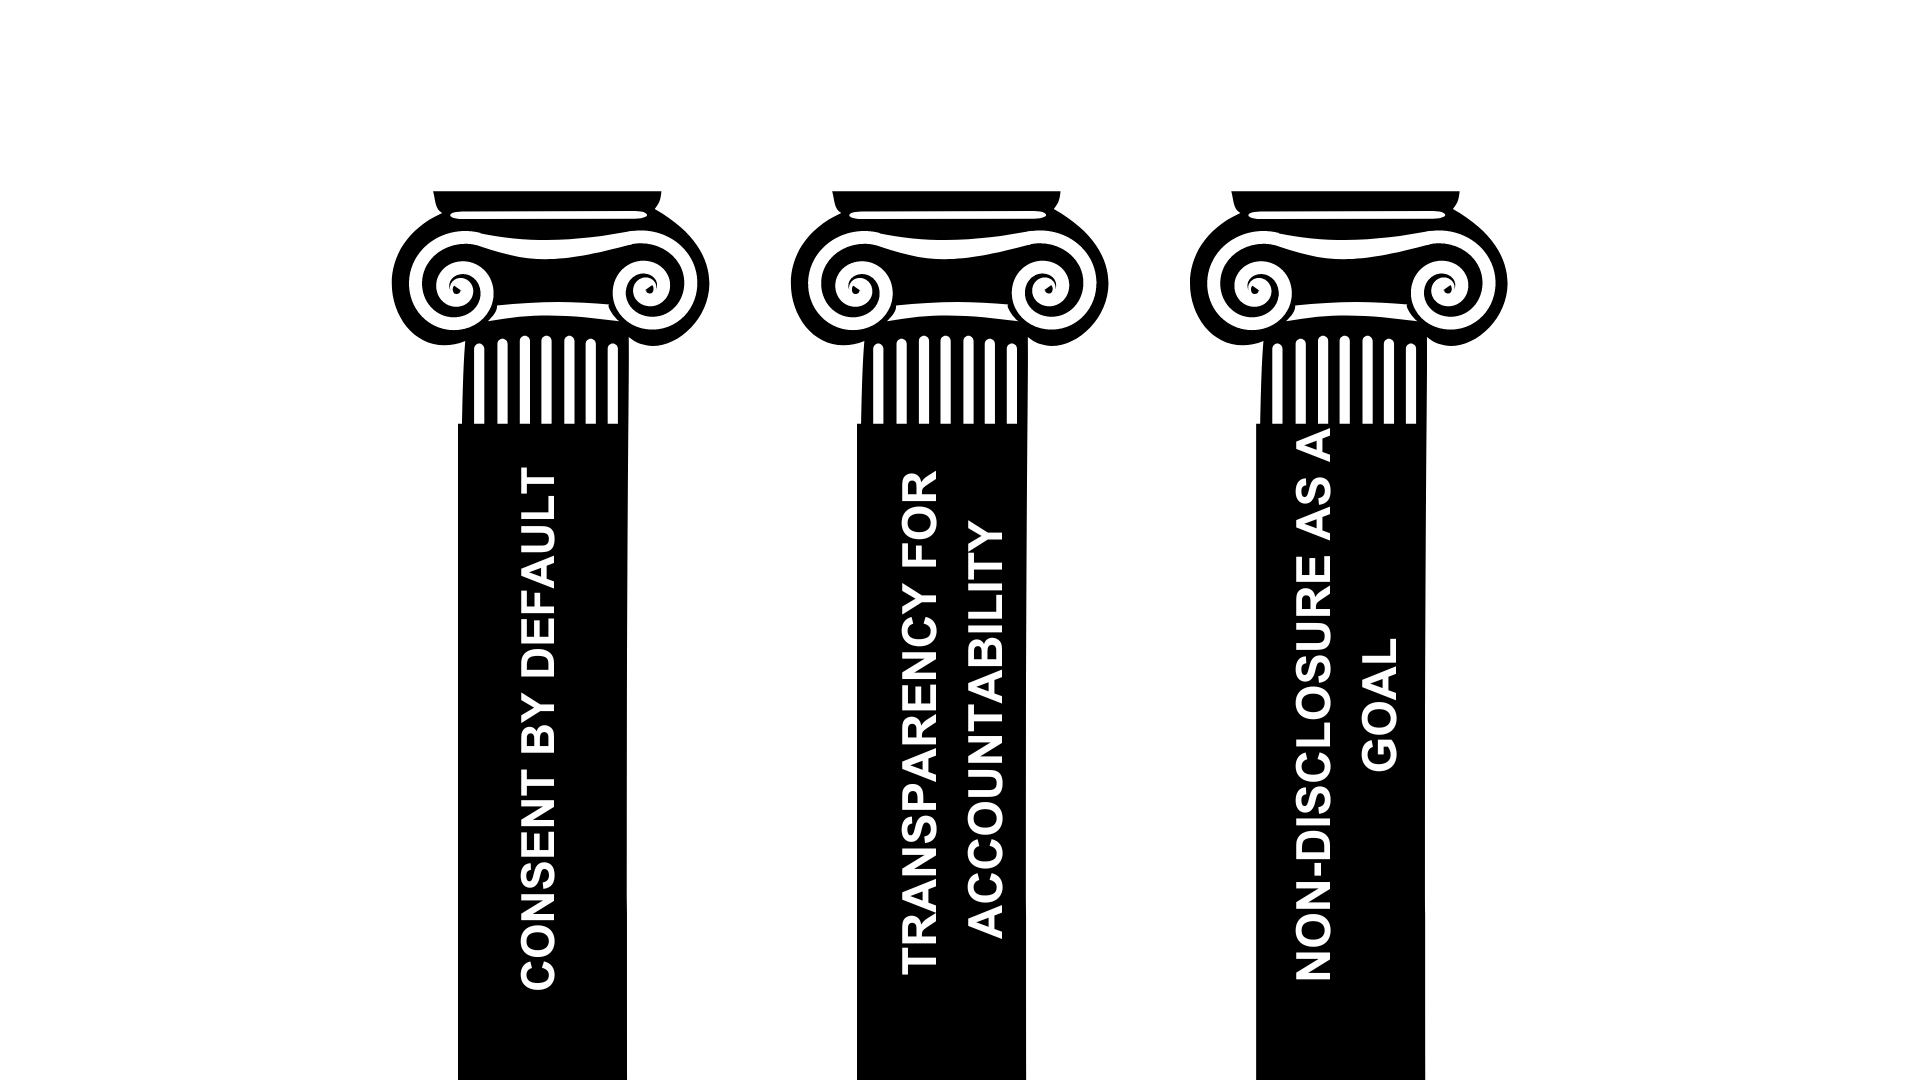
\includegraphics{images/png/pilares-do-FIM.png}}
    \fonte{O Autor}
    \label{fig:princilpes}
\end{figure}


O primeiro princípio, \emph{Consent by Default}, dita que todas as ações do fiduciário devem ser guiadas pelos consentimentos que o indivíduo definiu. Isso é implementado por meio de um artefato computacional chamado Política de Consentimento, que estabelece um conjunto de declarações feitas pelo usuário que definem o que pode ser feito com seus dados em termos de coleta, armazenamento e compartilhamento com outras entidades. Por meio deste artefato, o Fiduciário consegue decidir quais credenciais são mais adequadas para serem usadas em determinados contextos, seguindo a orientação do que o titular considera sensível sobre seus dados, possibilitando que ele não perca o controle sobre sua identidade digital. Essa política pode ser definida previamente, antes que as interações entre o usuário e \acs{SP} ocorram, ou sob demanda, caso o Fiduciário não consiga determinar claramente se sua ação pode ou não prejudicar a pessoa.

À primeira vista, a introdução de uma nova entidade responsável pelo gerenciamento dos dados pode parecer um retrocesso, retirando o controle dos indivíduos sobre suas próprias credenciais. Contudo, o objetivo é proporcionar suporte àqueles que enfrentam dificuldades ou preferem não se preocupar com as exigências de segurança relacionadas à manutenção de credenciais. As Políticas de Consentimento são projetadas para garantir que os titulares dos dados tenham todo o controle desejado, permitindo que flexibilizem ou restrinjam as ações do Fiduciário. Dessa forma, o Fiduciário pode atuar tanto como uma carteira digital presente nos modelos de \acs{SSI} quanto como um elo de confiança, ciente de suas responsabilidades e deveres, capacitado a tomar as melhores decisões em benefício do dono dos dados.

O segundo princípio, \emph{Transparency for Accountability}, estabelece que deve ser viável rastrear de forma precisa as ações realizadas sobre determinados dados, especificando o momento em que ocorreram e para quais finalidades foram utilizadas. Para esse propósito, é definido um artefato computacional denominado \emph{Evidências}, que serve para auditar toda e qualquer atividade realizada pelo fiduciário com os dados dos utilizadores. Através desse mecanismo, é possível realizar um processo sistemático de exame e avaliação das atividades e modificações de dados efetuadas pelo fiduciário, com o objetivo de verificar a conformidade com as políticas de consentimento e boas práticas, bem como avaliar a eficácia, eficiência e integridade dessas manipulações.

Ao permitir que o Fiduciário tome decisões de forma autônoma, ele pode se basear em solicitações anteriores semelhantes ou em outras métricas, visando reduzir as interrupções constantes aos usuários. Contudo, a autonomia conferida ao Fiduciário não o isenta de cometer erros na utilização dos dados dos indivíduos. Na prática, essa autonomia e os registros das ações garante ao beneficiário que seu representante será responsabilizado caso ocorra qualquer atitude delituosa. Adicionalmente, um aspecto significativo deste novo artefato é a sua capacidade de aprimorar a rastreabilidade das ações de um invasor que consiga comprometer o ambiente de execução do Fiduciário e conseguisse agir como tal agente. Isso se deve ao fato de que todas as atividades realizadas pelo Fiduciário serão registradas de forma detalhada, permitindo uma análise minuciosa e precisa das ações executadas durante a intrusão.

O terceiro princípio, \emph{Non-Disclosure as a Goal}, determina que o principal objetivo do modelo é manter a confidencialidade e evitar a revelação de determinadas informações, seja na construção de novos protocolos ou interfaces que utilizam o modelo como estrutura. Para alcançar esse objetivo, três mecanismos podem ser empregados: Divulgação Seletiva, \acs{ZKP} (Prova de Conhecimento Zero) e Seleção de Ambiente de Execução. Embora cada um desses mecanismos possa ser aplicado individualmente, a combinação deles potencializa significativamente o grau de preservação das informações dos beneficiários.

A primeira estratégia fundamenta-se na capacidade do Fiduciário de revelar apenas partes específicas das informações do usuário, sem expor a totalidade de seus dados. Para alcançar esse objetivo, busca-se a utilização de \acs{VC} que disponibilizem mecanismos para a construção de \acs{VP} que contenham apenas um subconjunto de atributos, em vez de incluir todos os atributos disponíveis. A segunda estratégia é baseada na utilização de  \acs{ZKP}, conforme detalhado na \autoref{section:zkp}, pois apesar de também ser uma solução de divulgação seletiva, essa abordagem reduz de forma significativa a exposição de dados em comparação à seleção de atributos para uma \acs{VP}. Independentemente do mecanismo adotado, o modelo visa proporcionar ao indivíduo maior controle sobre seus dados pessoais, permitindo-lhe fornecer apenas as informações estritamente necessárias e, assim, minimizar a exposição de dados supérfluos ou potencialmente invasivos.

A terceira estratégia explora a possibilidade de processamento de dados fora do ambiente do \acs{SP}. Tradicionalmente, o processamento de dados relacionados à identidade ocorre em um ambiente de confiança controlado pelo \acs{SP}, sem oferecer ao usuário a opção de escolher o ambiente que considera mais seguro, resultando na transferência obrigatória de dados de um ambiente para outro. No entanto, o modelo proposto introduz duas alternativas: a primeira permite que o processamento ocorra em um ambiente de confiança do próprio titular dos dados, em consonância com a proposta de \citeonline{opal}. A segunda possibilita a computação colaborativa entre diferentes entidades por meio de técnicas seguras de Computação Multipartidária, conhecida em inglês como \sigla{MPC}{Multiparty Computation}, assegurando que os dados de cada participante permaneçam privados e confidenciais ao longo de todo o processo. 


% Figura do modelo Fiduciário (Conceitual)
\begin{figure}[htb]
    \caption{Modelo Fiduciário.}
    \centering
    \resizebox{0.8\linewidth}{!}{\begin{minipage}[b]{0.5\linewidth}
    \centering
    \begin{tikzpicture}[roundnode/.style={circle, draw=black, very thick, minimum size=20mm, align=center},]
        % Nodes
        \node[roundnode]      (idp)                            {IdP};
        \node[roundnode]      (sp)     [below right=3cm and 1cm of idp]  {SP}; % Adjusted positioning
        \node[roundnode]      (fid)    [below left=3cm and 1cm of idp]  {Fiduciário}; % Adjusted positioning
        \node[roundnode]      (usr)    [left=of fid]  {usuário};
        
        % Lines
        \draw[<->] (idp) -- (fid);
        \draw[<->]  (fid) -- (sp);
        \draw[->, dashed] (sp) edge[bend right=5, draw=none] coordinate[at start](sp-b) coordinate[at end](idp-b) (idp)
                  edge[bend left=5, draw=none] coordinate[at start](sp-t) coordinate[at end](idp-t) (idp)
              (sp-t) -- (idp-t);
        \draw[<->] (fid) edge[bend right=-5, draw=none] coordinate[at start](fid-b) coordinate[at end](usr-b)(usr)
              edge[bend left=-4, draw=none] coordinate[at start](fid-t) coordinate[at end](usr-t) (usr)
             (fid-t) -- (usr-t);
        \draw[<-, double, dashed] (usr) edge[bend right=5, draw=none] coordinate[at start](usr-b) coordinate[at end](fid-b) (fid)
              edge[bend left=-10, draw=none] coordinate[at start](usr-t) coordinate[at end](fid-t) (fid)
             (usr-t) -- (fid-t);
    \end{tikzpicture}
\end{minipage}
}
    \vspace{0.5cm}
    \fonte{Inspirado em \citeonline{revisao-ssi-frederico}}
    \label{fig:fiduciary-model}
\end{figure}

\section{Protocolos de Identidade Digital}\label{subsection:protocolos}

\subsection{OAuth 2.0}\label{subsubsection:oauth}

OAuth 2.0 é um protocolo  de autorização que fornece à aplicações a capacidade de acessar um recurso de usuário por meio de tokens, evitando que o indivíduo precise compartilhar a sua credencial de acesso com aplicação. Dessa forma, não há necessidade de compartilhar credenciais sensíveis \cite{oauth}. Por exemplo, um leitor pode autorizar um aplicativo de notícias à acessar sua conta ou realizar postagens em seu nome na sua conta de sua rede social sem revelar para o aplicativo qual é a senha. Caso o aplicativo de notícias sofra algum tipo de vazamento de dados, a senha da rede social desse leitor continua resguardada no \acs{IdP}, a rede social.

Para que o protocolo funcione adequadamente, quatro papéis principais são essenciais no processo. Primeiramente, temos o \textbf{Proprietário do recurso}, que corresponde ao indivíduo que deseja autorizar uma aplicação a acessar seus dados. No cenário ilustrativo de leitura de notícias, o Proprietário do recurso seria o leitor que pretende permitir que um aplicativo acesse suas preferências de leitura. Em segundo lugar, o \textbf{Cliente} é a aplicação que almeja utilizar os dados do indivíduo. Mantendo o exemplo anterior, o cliente seria o aplicativo de notícias que deseja acessar as preferências do leitor para personalizar o conteúdo apresentado. O terceiro papel é desempenhado pelo \textbf{Servidor de Autorização}, que é o responsável por autenticar o usuário e fornecer tokens que permitem ao cliente acessar os recursos do indivíduo. Este servidor atua como uma ponte de confiança entre o Proprietário do recurso e o cliente, assegurando que apenas aplicativos devidamente autorizados possam acessar os dados. Finalmente, temos o \textbf{Servidor de Recurso}, que é o servidor responsável por armazenar os dados do indivíduo. Frequentemente, o servidor de recurso coincide com o servidor de autorização, embora possam ser distintos dependendo da arquitetura do serviço implementado. Comparando com o modelo terceirizado da \autoref{fig:identity-models}, o Servidor de Autorização e o Servidor de Recurso correspondem ao \acs{IdP}, o Proprietário do recurso representa o Usuário, e o \acs{SP} é o Cliente.

Além desses papéis, o protocolo utiliza tokens, credenciais que representam a autorização, para gerenciar o acesso aos recursos. Alguns deles são \textbf{Código de Autorização}, \textbf{Token de Acesso} e o \textbf{Token de Atualização}. O Código de Autorização (Authorization Grant) é um token fornecido ao cliente após a autenticação do usuário perante o servidor de autorização. Este código é utilizado pelo cliente para obter um Token de Acesso e se trata de uma sequência de caracteres que comprova que o usuário autorizou o cliente a agir em seu nome. O Código de Acesso (Access Token) é o token que determina o tipo de acesso que o cliente terá sobre os recursos do indivíduo. Este token geralmente inclui informações sobre o escopo específico de acesso, o tempo de validade e outros atributos relevantes; no entanto, o provedor pode personalizar o conteúdo do token conforme suas necessidades. É com este token que o cliente realiza efetivamente o acesso aos dados. Por fim, os tokens de atualização (Refresh Tokens) permitem que a aplicação obtenha novos Tokens de Acesso sem a necessidade de reautenticação do usuário. O uso de Tokens de Atualização reduz a frequência com que o usuário precisa interagir com o processo de autenticação, melhorando a segurança, já que o usuário não precisa fornecer suas credenciais repetidamente.

O OAuth 2.0 utiliza o protocolo \sigla{HTTP}{HyperText Transfer Protocol} para transmitir parâmetros durante o processo de autorização. Quando um cliente inicia uma solicitação de autorização, ele redireciona o navegador do usuário para o Ser3vidor de Autorização utilizando o método \acs{HTTP} GET, incluindo alguns parâmetros na URL da requisição. Três parâmetros importantes nesse contexto são o \textbf{\texttt{\texttt{scope}}}, \textbf{\texttt{response\_type}} e \textbf{\texttt{client\_id}}. O parâmetro \texttt{scope} define o nível de acesso que o cliente está solicitando, especificando as permissões desejadas. Por exemplo, uma aplicação pode solicitar acesso apenas à leitura de emails ou à leitura e escrita de contatos. 

O parâmetro \texttt{response\_type} define o fluxo de mensagens para autenticação e autorização, determinando o tipo de resposta que o Cliente deve esperar do Servidor de Autorização. Existem quatro fluxos distintos: \textbf{Fluxo de Código de Autorização} (Authorization Code Flow), \textbf{Fluxo Implícito} (Implicit Flow), \textbf{Fluxo de Credenciais de Senha do Proprietário do Recurso} (Resource Owner Password Credentials Flow) e \textbf{Fluxo de Credenciais do Cliente} (Client Credential Flow). Assim, dependendo \texttt{response\_type} escolhido e outros parâmetros, algum desses fluxo poderá ser utilizado. Por exemplo, se o \texttt{response\_type} é \texttt{code}, utiliza-se o Fluxo de Código de Autorização, onde o cliente recebe um código de autorização que será trocado por um Token de Acesso. Já se for o \texttt{response\_type}=\texttt{token} é utilizado no Fluxo Implícito, onde o cliente recebe diretamente um Token de Acesso.

Outro parâmetro crucial é o \texttt{client\_id}, que identifica de forma única a aplicação cliente que está solicitando acesso aos recursos do usuário. Este identificador é fornecido pelo Servidor de Autorização quando a aplicação é registrada. Em combinação com o \texttt{client\_secre}t, que é um segredo conhecido apenas pela aplicação e pelo Servidor de Autorização, o \texttt{client\_id} ajuda a autenticar a aplicação durante o processo de obtenção do Token de Acesso. Além disso, as requisições ao servidor de autorização geralmente incluem a \texttt{redirect\_uri}, que é a URL para a qual o usuário será redirecionado após o processo de autenticação e autorização. Esta URL deve ser registrada previamente no Servidor de Autorização e corresponder exatamente ao que foi registrado para evitar ataques de redirecionamento malicioso.

Há também a definição de vários endpoints usados ao longo do processo de autorização. O \textbf{Authorization Endpoint} é o URL onde o usuário é redirecionado para fornecer o consentimento e autenticar. Este endpoint processa as solicitações de autorização e emite Códigos de Autorização ou tokens, dependendo do fluxo. O \textbf{Token Endpoint} é utilizado para trocar um Código de Autorização por um Token de Acesso, sendo também usado para renovar Tokens de Acesso expirados. O \textbf{Resource Endpoint} é onde os recursos protegidos são acessados. O cliente usa o Token de Acesso para solicitar recursos do servidor de recursos.

Esses papéis, artefatos, parâmetros e endpoints permitem construir uma implementação robusta do OAuth 2.0, assegurando acesso seguro e controlado a recursos, sem comprometer as credenciais dos usuários. O protocolo é flexível e adaptável, equilibrando segurança e usabilidade conforme as necessidades das aplicações.

A \autoref{fig:oauth}, descrita a seguir, demonstra o funcionamento do \emph{Fluxo de Código de Autorização}. Nesse fluxo, ocorre a obtenção de um \emph{Código de Autorização}, que é subsequentemente trocado por um Token de Acesso. Na figura, observa-se que, após o usuário selecionar o \acs{IdP} de sua preferência, como o Facebook, ele é redirecionado pelo navegador por meio de uma requisição realizada pelo \acs{SP} (Cliente). A partir desse ponto, o fluxo descrito na imagem é iniciado.
% Figura dos funcionamento do oauth
\begin{figure}[htb]
    \caption{Fluxo de Código de Autorização no OAuth}
    \centering
    
    \resizebox{0.8\linewidth}{!}{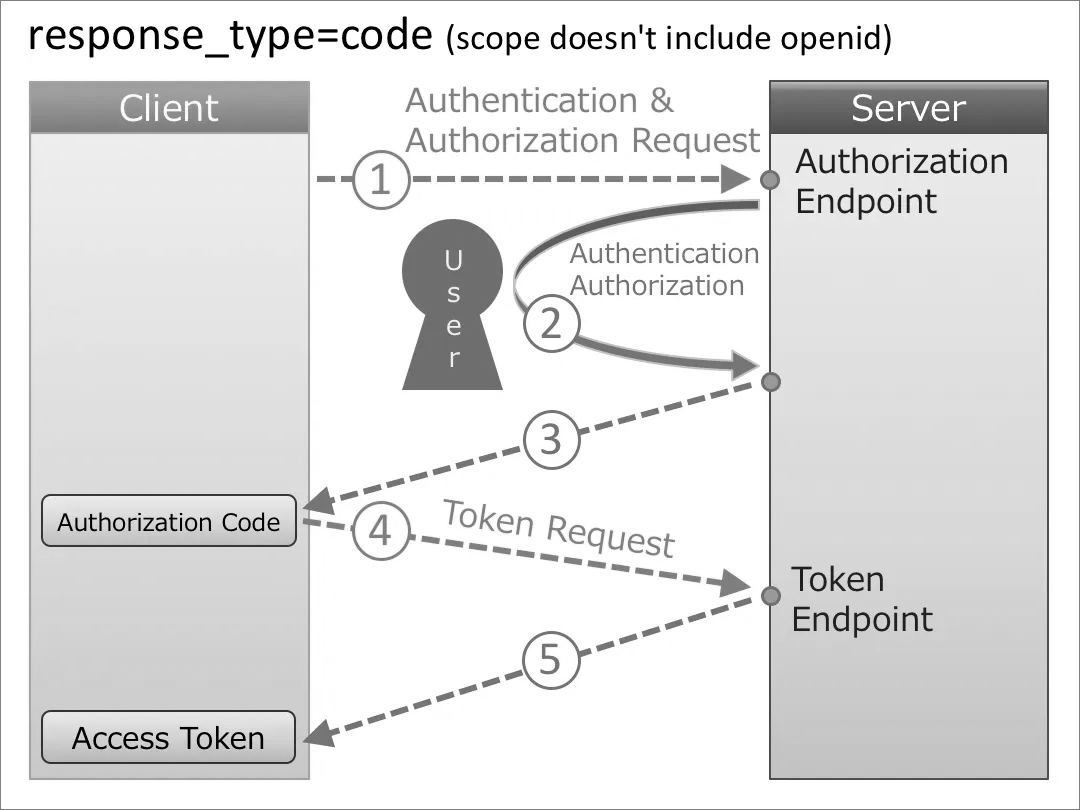
\includegraphics{images/png/oauth.png}}

    \fonte{\citeonline{OAuthImage2024}}
    \label{fig:oauth}
\end{figure}


\begin{enumerate}
    
    \item O serviço Web (Cliente) redireciona o utilizador para a tela de login no Servidor de Autorização, fornecendo seu identificador, \texttt{client\_id}.
    
    \item O indivíduo autentica-se perante o Servidor de Autorização e concede acesso ao seu recurso para o aplicação.
    
    \item O Servidor de Autorização emite o Código de autorização, que é encaminhado ao cliente via redirecionamento no navegador do usuário.
    
    \item A aplicação solicita o token de acesso correspondente ao seu código de autorização para o Servidor de Autorização. 
    
    \item O Servidor de Autorização encaminha o código de acesso. Nesse ponto, a troca é feita diretamente entre o backend da aplicação e o Servidor de Autorização, sem passar pelo navegador do usuário.

\end{enumerate}

Ao final do fluxo, a aplicação cliente utiliza o Token de Acesso para realizar requisições ao Servidor de Recursos, sendo autorizada a acessar apenas os recursos específicos concedidos pelo usuário. 

\subsection{OpenID Connect}\label{subsec:OIDC}

\sigla{OIDC}{OpenID Connect} é um protocolo de autenticação baseado na família de especificações OAuth 2.0, permitindo que as aplicações autentiquem usuários e obtenham informações sobre eles, proporcionando uma experiência de \acs{SSO} \cite{openid}. Ele é amplamente adotado por grandes provedores de identidade, como Google, Microsoft e Facebook, proporcionando uma interoperabilidade robusta e simplificada entre diversas plataformas e serviços, facilitando a integração e melhorando a segurança na autenticação de usuários em aplicações web e móveis.

Um novo token é definido chamado de \texttt{id\_token} para identificar os usuários para a aplicação. Este token está organizado em uma estrutura de \sigla{JWT}{JSON Web Token} que contém informações sobre a autenticação do usuário, incluindo o emissor do token, o público-alvo representado por um \texttt{client\_id}, um identificador único do usuário final no IdP, a data e hora da autenticação e os tempos de emissão e expiração do token. Para emitir esse token, novos fluxos também são definidos estendendo a especificação do parâmetro \texttt{response\_type}. No OAuth o valor de \texttt{response\_type} é code ou token. O \acs{OIDC} adiciona o \texttt{id\_token}, e permite qualquer combinação de code, token e \texttt{id\_token}. Um valor especial, none, também é adicionado. 

Também é adicionado o valor \textbf{openid} para o parâmetro \texttt{scope}, que é utilizado para definir as permissões específicas que uma aplicação está solicitando em relação aos dados do usuário. Especificamente, este valor permite que a aplicação obtenha um \texttt{id\_token}, que contém informações autenticadas sobre o usuário, como seu identificador único, e possivelmente outras informações adicionais se escopos adicionais como profile, email ou address forem incluídos. O escopo profile permite que a aplicação acesse uma variedade de informações de perfil básicas sobre o usuário. Isso pode incluir o nome completo, apelido, foto de perfil, gênero, data de nascimento, idioma preferido e outras informações de perfil. A inclusão deste escopo proporciona uma visão mais completa do usuário. O escopo email concede à aplicação acesso ao endereço de e-mail do usuário e a verificação se o endereço de e-mail foi verificado. Especificamente, a aplicação pode obter o endereço de e-mail e um indicador booleano (email\_verified) que informa se o endereço foi verificado. Isso é útil para aplicações que necessitam de um contato confiável com o usuário ou para validação de identidade. O escopo address permite que a aplicação acesse o endereço físico do usuário. Isso pode incluir informações como a rua, cidade, estado, código postal e país. A inclusão deste escopo é útil para aplicações que requerem informações de envio ou para personalizar ofertas e serviços baseados na localização do usuário.

Ademais, também é exigido a obrigatoriedade do \texttt{redirect\_uri} como medida de segurança para garantir que as Respostas da Autorização sejam enviadas apenas para URLs previamente autorizados. Isso ajuda a prevenir ataques como a homem no meio (man-in-the-middle) e a ataque de redirecionamento, onde um atacante poderia tentar interceptar ou redirecionar as respostas de autorização para um local malicioso. 

A \autoref{fig:openid}, descrita a seguir, demonstra o funcionamento do Fluxo de Código de Autorização no conxtexto do \acs{OIDC}. Nesse fluxo, ocorre a obtenção de um Código de Autorização, que é subsequentemente trocado por um \texttt{id\_token}.
Semelhante ao OAuth 2.0, após o usuário selecionar o \acs{IdP} de sua preferência, como o Google, ele é redirecionado pelo navegador por meio de uma requisição realizada pelo \acs{SP} (Cliente). A partir desse ponto, o fluxo descrito na imagem se inicia.

% Figura com o funcionamento do OIDC

\begin{figure}[htb]
    \caption{Fluxo de Código de Autorização no OIDC.}
    \centering
    \resizebox{0.5\linewidth}{!}{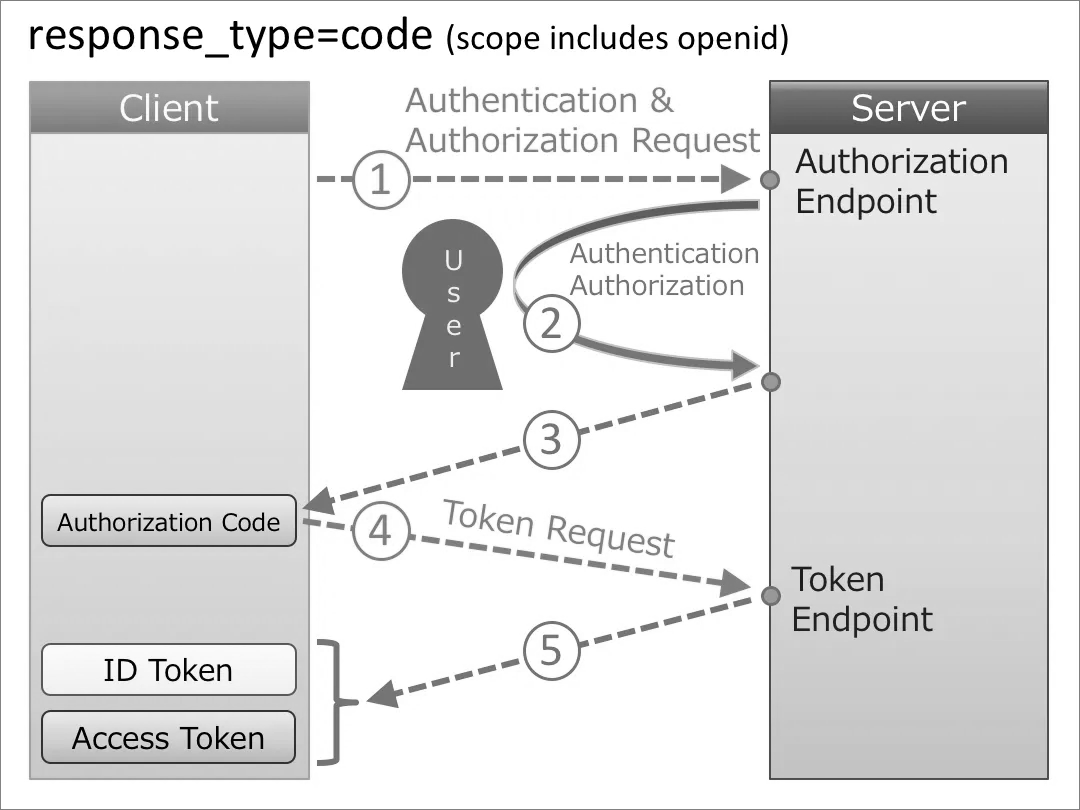
\includegraphics{images/png/openid.png}}
    \label{fig:openid}
    \fonte{\citeonline{OpendIDImage2024}}
\end{figure}


\begin{enumerate}
    
    \item O serviço Web (Cliente) redireciona o utilizador para a tela de login no Servidor de Autorização, fornecendo seu identificador, \texttt{client\_id}.
    
    \item O indivíduo autentica-se perante o Servidor de Autorização, fornecendo suas credenciais de acesso, como nome de usuário e senha.
    
    \item O Servidor de Autorização emite o Código de autorização, que é encaminhado ao cliente via redirecionamento no navegador do usuário.
    
    \item A aplicação solicita o token de acesso correspondente ao seu código de autorização para o Servidor de Autorização. 
    
    \item O Servidor de Autorização encaminha o código de acesso e o \texttt{id\_token}. Nesse ponto, a troca é feita diretamente entre o backend da aplicação e o Servidor de Autorização, sem passar pelo navegador do usuário.

\end{enumerate}

Ao final do fluxo, a aplicação cliente pode utilizar o \emph{UserInfo Endpoint} para obter informações adicionais sobre o usuário, como nome, e-mail ou outros dados, utilizando o código de acesso recebido. Após essa etapa, o usuário é autenticado com sucesso e redirecionado para a página do serviço, onde tem acesso aos recursos autorizados de acordo com seu perfil.

\subsection{OIDC4VC: O OpenID Connect no modelo SSI }\label{subsec:oidc4vc}

O \sigla{OIDC4VC}{OpenID Connect com Credenciais Verificáveis} representa um conjunto de protocolos avançados projetados para estabelecer um ecossistema de \acs{SSI} \cite{OIDC4VCWhitepaper2022}. Esse sistema capitaliza as funcionalidades robustas e amplamente validadas do OpenID Connect, amplamente adotado no modelo terceirizado de autenticação, oferecendo uma experiência segura e eficiente para a gestão de identidades digitais. Ao integrar Credenciais Verificáveis e, consequentemente, Apresentações Verificáveis ao \acs{OIDC}, o \acs{OIDC4VC} proporciona um mecanismo poderoso e flexível, permitindo que os indivíduos autentiquem e compartilhem suas identidades com uma combinação de segurança, privacidade e conveniência.  Essa abordagem garante que apenas os dados estritamente necessários sejam compartilhados em cada transação, oferecendo aos usuários um controle refinado sobre suas interações digitais.

O problema do protocolo \acs{OIDC} dentro do modelo Terceirizado é que ele levanta preocupações significativas sobre a redução de privacidade causada pela centralização de controle de credencias e a dificuldade de gerenciamento das mesmas em diferentes provedores. Durante o processo de autenticação usando o \acs{OIDC}, informações sensíveis sobre o indivíduo podem ser inadvertidamente compartilhadas com o \acs{IdP} que atua como Servidor de Autorização, como detalhes sobre quais serviços online a pessoa acessa \cite[Página 7]{OIDC4VCWhitepaper2022}. Isso ocorre porque a sua arquitetura centralizada concentra o controle das identidades digitais no \acs{IdP} (Servidor de Autorização).

Cada provedor emite e gerencia suas próprias credenciais de forma isolada, o que impede a unificação ou combinação de atributos provenientes de diferentes fontes em uma única credencial ou token. Por exemplo, um usuário pode ter uma credencial emitida por um banco que contém informações financeiras e outra credencial emitida por uma rede social com dados pessoais. No modelo \acs{OIDC}, esses atributos permanecem separados, e o usuário não tem uma maneira eficiente de combiná-los em um único artefato que possa ser utilizado para uma verificação mais simplificada de sua identidade em diversos contextos. Essa limitação não apenas aumenta a complexidade do gerenciamento de identidades, mas também restringe a flexibilidade e a utilidade das credenciais digitais, dificultando a criação de experiências de usuário mais integradas e seguras.

O \acs{OIDC4VC} visa abordar esses desafios de maneira eficaz, especialmente ao redefinir a responsabilidade do envolvida na emissão, armazenamento e apresentação das credenciais. Ao restringir o papel de \acs{IdP} a apenas emitir e delegar aos usuários a tarefa de armazenar e apresentar suas credenciais por meio de carteiras digitais, o novo ecossistema permite que os indivíduos exerçam um controle mais rigoroso sobre suas informações pessoais. Essa mudança possibilita que os usuários compartilhem seus dados diretamente com os serviços, de acordo com suas necessidades, garantindo que apenas as informações estritamente necessárias sejam divulgadas no momento oportuno. Essa abordagem fortalece a autonomia do usuário e promove um ambiente mais seguro e privado para a gestão de identidades digitais.

Ao empregar \acs{VP}s, os protocolos mitigam o problema da fragmentação das credenciais emitidas por diferentes provedores, possibilitando a unificação e combinação de atributos em um único artefato digital. Essa abordagem permite que o usuário consolide informações derivadas de múltiplas credenciais emitidas por diversas fontes, como exemplificado pela integração de dados provenientes de um banco e de uma rede social em uma única \acs{VP}. Dessa forma, o usuário pode fornecer, em suas interações com serviços online, uma representação mais completa e integrada de sua identidade. As \acs{VP} aprimoram o gerenciamento de identidades ao permitir que o usuário selecione e combine apenas os atributos necessários para cada contexto específico, promovendo uma experiência mais fluida e segura, ao mesmo tempo em que preservam a privacidade e mantêm o controle sobre as informações compartilhadas.

\subsubsection{Ecossistema}\label{subsubsection:ecossistema-oidc4vc}

Para sustentar essa estrutura, o \acs{OIDC4VC} estabelece uma série de protocolos e extensões que integram as funcionalidades do OpenID Connect ao modelo de Credenciais Verificáveis, conforme ilustrado na  \autoref{fig:protocol-opid4vc}.

% Figura com os três protocolos do OIDC4VC
\begin{figure}[htb]
    \caption{Ecossistema do OIDC4VC.}
    \centering
    
    \resizebox{\linewidth}{!}{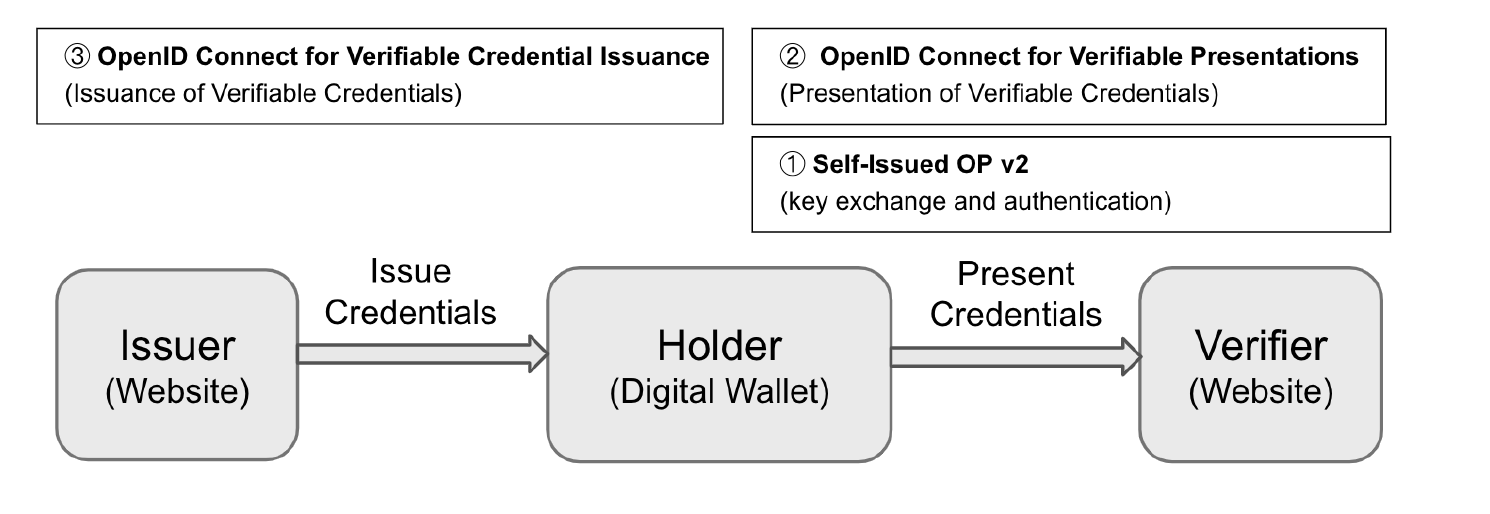
\includegraphics{images/png/protocol-of-OID4VC.png}}
    
    \label{fig:protocol-opid4vc}
    \fonte{\citeonline{OIDC4VCWhitepaper2022}}
\end{figure}


\begin{enumerate}

    \item \textbf{\sigla{SIOPv2}{Self-Issued OpenID Provider v2}}: É uma especificação que permite aos usuários atuarem como seus próprios \acs{IdP}, emitindo e gerenciando suas credenciais diretamente sem depender de um provedor de identidade terceirizado. Com ele o usuário pode gerar e assinar atributos como nome, e-mail, sem que sejam verificadas por uma entidade central. Além de conseguir provar que realmente controla a chave privada associada a essa assinatura (prova de posse) \cite{SIOPv2023}. 

    O \acs{SIOPv2} permite uma ampla variedade de arquiteturas de carteiras. Por exemplo, as carteiras podem ser executadas no dispositivo do usuário, mas também podem ser hospedadas na nuvem. A experiência do usuário pode ser fornecida por meio de um aplicativo móvel ou uma aplicação web. Do ponto de vista do protocolo, elas podem utilizar todos os fluxos do OpenID Connect, ou seja, há uma grande variedade de opções para atender às necessidades da respectiva implantação e dos casos de uso.
    
    \item \textbf{\sigla{OIDC4VP}{OpenID para Apresentações Verificáveis}}: Extensão do OpenID Connect para permitir os serviços solicitarem e receberem Apresentações Verificáveis \cite{OIDC4VP2023}.
    
    \item \textbf{\sigla{OIDC4CI}{OpenID para Emissão de Credenciais Verificáveis}}: Esta especificação propõe uma API destinada à emissão de \acs{VC}s em diversos formatos, incluindo o do W3C \cite{data-model-w3c}. As \acs{VC}s são emitidas por meio de uma carteira digital, previamente autorizada pelo usuário através do protocolo OAuth 2.0. Essa abordagem visa aproveitar as características comprovadas de segurança, simplicidade e flexibilidade inerentes ao protocolo OAuth 2.0 \cite{OIDC4CI2023}.

    Embora seja viável autorizar a emissão de credenciais conforme os serviços acessados requeiram informações do usuário, como ocorre no modelo terceirizado atual, a proposta das carteiras digitais visa proporcionar um maior controle ao usuário. Nesse modelo, os usuários armazenarão suas credenciais e gerarão \acs{VP}s individualizadas para cada serviço utilizado, o que reduz significativamente a possibilidade de os \acs{IdP}s monitorarem quais serviços são acessados e com que frequência isso ocorre.
    
\end{enumerate}

\subsubsection{OIDC4VP}\label{subsubsection:oidc4vp}

\acs{OIDC4VP} amplia as capacidades do OpenID ao permitir a apresentação de Credenciais Verificáveis na forma de Apresentações Verificáveis. Essa extensão oferece uma série de funcionalidades que reforçam a flexibilidade e a interoperabilidade do sistema, como a compatibilidade com todos os fluxos do OpenID Connect, o suporte a diferentes formatos de \acs{VC}s e \acs{VP}s, a capacidade de utilizar múltiplos métodos de transporte e o reaproveitamento do parâmetro claims para definir a sintaxe de solicitações. Nos parágrafos subsequentes, será detalhado cada um desses itens para fornecer uma compreensão mais profunda de suas funcionalidades e benefícios.

O protocolo é projetado para ser compatível com todos os fluxos do OpenID Connect. Isso significa que, independentemente do fluxo de autenticação escolhido, desde aqueles mais comuns como o Fluxo de Código de Autorização até naqueles em que o usuário é seu próprio provedor de identidade (\acs{SIOPv2}), \acs{OIDC4VP} pode ser integrado de maneira eficaz, garantindo flexibilidade e interoperabilidade.  Ademais, a sintaxe das solicitações reaproveita o parâmetro claims do \acs{OIDC} e utiliza a especificação DIF Presentation Exchange \cite{presentation-exchange} para formatar \acs{VP}s. 

O sistema oferece suporte a diferentes formatos de credenciais e apresentações, permitindo codificações em \sigla{JSON}{JavaScript Object Notation} ou \sigla{JSON-LD}{JSON for Linked Data}, bem como assinaturas utilizando \sigla{JWS}{JSON Web Signature} ou Linked Data Proofs. A capacidade de operar com diversos formatos e métodos de assinatura amplia significativamente a interoperabilidade do sistema, facilitando sua adaptação a diferentes padrões e requisitos técnicos. Por exemplo, o \acs{JSON} é amplamente utilizado em diversas aplicações web devido à sua simplicidade e eficiência \cite{JSONrfc82592017}, enquanto o \acs{JSON-LD} é preferido em contextos que demandam maior semântica e interconectividade de dados \cite{jsonld112020}. A escolha de formato é uma característica importante, porque determina se uma credencial suporta propriedades que reduzem a exposição de dados \cite{OIDC4CI2023Authlete}, como a Divulgação Seletiva e \acs{ZKP} descritas na \autoref{subsection:auto-soberano}.

A flexibilidade robusta na transmissão de \acs{VC}s e \acs{VP}s, suportando múltiplos métodos de transporte, é uma característica essencial. As informações podem ser integradas diretamente no \texttt{id\_token} ou na resposta do Userinfo, permitindo uma integração transparente com os fluxos de autenticação já existentes. Alternativamente, as credenciais podem ser transmitidas por meio de um token dedicado, o \textbf{\texttt{redirect\_uri}}, que pode ser retornado juntamente com o \texttt{id\_token} a partir dos endpoints de autorização ou token. Independentemente da forma que essa \acs{VP} seja encaminhada, para que a carteira saiba quais atributos são necessários, dentro da Requisição de Autorização, é reutilizado o parâmetro claims do \acs{OIDC} para conter um \texttt{redirect\_uri} com um \textbf{presentation\_definition}. Esse último contém uma \sigla{DA}{Definição de Apresentação} \cite{presentation-exchange}, que é uma estrutura que define como as apresentações devem ser enviadas para o \acs{SP}.


\subsubsection{Funcionamento}{\label{subsubsection:oidc4vc}}

No contexto desta especificação, a Carteira desempenha a função de Servidor de Autorização OAuth 2.0 em relação ao \acs{SP}, que, por sua vez, atua como Cliente OAuth 2.0 \cite{OIDC4VP2023}. Essa distinção é significativa, pois, em outras especificações, como no \acs{OIDC4CI}, a Carteira assume o papel de Cliente OAuth 2.0. Ademais, com essa definição, os \acs{SP} podem usufruir dos mecanismos existentes para facilitar o registro de clientes, como especificado no \sigla{OIDC-D}{OpenID Connect Discovery} \cite{sakimura2023openidDiscovery} e \sigla{OIDC-DCR}{OpenID Connect Dynamic Client Registration} \cite{sakimura2023openid-dcr}

As especificações \acs{OIDC-D} e \acs{OIDC-DCR} desempenham papéis complementares no ecossistema de autenticação do OpenID Connect. O \acs{OIDC-D} possibilita que os clientes descubram automaticamente as configurações e endpoints do provedor de identidade por meio de um documento de descoberta, facilitando a configuração e integração com o sistema de autenticação. Já o OIDC Dynamic Client Registration permite que clientes sejam registrados de forma dinâmica e automática com o provedor de identidade, sem a necessidade de intervenção manual, o que é particularmente útil em ambientes com alta demanda de novos clientes. Juntas, essas especificações tornam a gestão de autenticação e autorização mais ágil, flexível e escalável.

O funcionamento desse protocolo é estruturado em dois fluxos distintos. O primeiro, denominado \textbf{same-device flow}, refere-se ao processo no qual o usuário apresenta uma credencial a um \acs{SP} utilizando o mesmo dispositivo em que sua carteira digital está instalada. Nesse fluxo, tanto o \acs{SP} quanto a Carteira interagem diretamente no dispositivo do usuário, empregando redirecionamentos simples para a troca da Solicitação de Autorização (Authorization Request) e da Resposta de Autorização (Authorization Response) entre ambas as partes. Esse fluxo é exemplificado na figura \autoref{fig:samedevice}. O segundo fluxo, conhecido como \textbf{cross-device flow}, ocorre quando o \acs{SP} e a Carteira residem em dispositivos distintos. Nesse contexto, o \acs{SP} gera uma Solicitação de Autorização e a apresenta ao usuário na forma de um código QR (QR Code). O usuário, então, utiliza a Carteira em seu dispositivo para escanear o código QR e iniciar o processo de verificação, permitindo a continuidade da interação de forma segura e eficiente.

O protocolo introduz novos tipos de resposta (\texttt{response\_type}) para suportar a transmissão de tokens de apresentação verificável (\texttt{vp\_token}) em diferentes cenários de autenticação. Quando o valor de \texttt{response\_type} é \texttt{vp\_token}, a \acs{VP} é retornada diretamente na Resposta de Autorização (Authorization Response). No caso em que o valor de \texttt{response\_type} é \texttt{redirect\_uri} \texttt{id\_token} e o parâmetro \texttt{scope} contém \texttt{openid}, o \texttt{redirect\_uri} é retornado na Resposta de Autorização juntamente com um ID Token autoemitido, conforme definido no \cite{SIOPv2023}. Além disso, quando o \texttt{response\_type} é \textbf{code}, seguindo o Fluxo de Código de Autorização, o \texttt{redirect\_uri} é fornecido na Resposta de Token (Token Response), após a troca bem-sucedida do código de autorização pelo token correspondente. Nesse exemplo, o \texttt{response\_type} é \texttt{redirect\_uri}.

\begin{figure}[htb]
    \caption{Fluxo com Carteira e \acs{SP} no mesmo dispositivo}
    \centering
    
    \resizebox{\linewidth}{!}{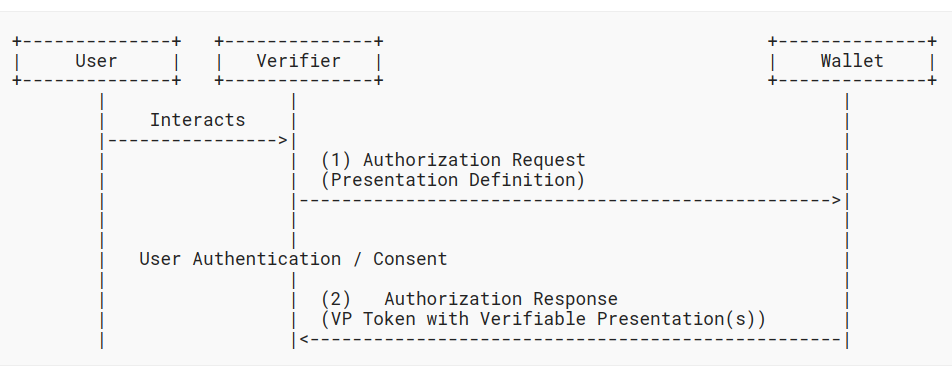
\includegraphics{images/png/same-device.png}}
    
    \label{fig:samedevice}
    \fonte{\citeonline{OIDC4VP2023}}
\end{figure}

\begin{enumerate}

    \item O \acs{SP} representado por um verficador, realiza um \textbf{Solicitação de Autorização} (Authorization Request) no \textbf{Endpoint de Autorização} para a carteira digital. 
    Nesse caso, o parâmetro \texttt{response\_type} inclui o valor \texttt{vp\_token}, enquanto o \texttt{presentation\_definition} contém a \acs{DA} que define os critérios que as \acs{VP}s devem cumprir, como o tipo de credencial exigido, o formato de apresentação e os atributos específicos das credenciais que devem ser compartilhados.    % Nesse caso, \texttt{response\_type} contém \texttt{redirect\_uri} e o \texttt{presentation\_definition} com a \acs{DA} com quais requisitos as \acs{VP}s devem cumprir, como o tipo de credencial utilizada, o formato em que devem ser apresentadas, quais atributos individuais dentro dessas credenciais devem ser apresentados. 
    
    \item A Carteira retorna a Resposta de Autorização, \emph{Authorization Response}. Nesse caso, com o \texttt{response\_type} definido como \texttt{vp\_token}, o valor de \texttt{vp\_token} é enviado diretamente.

    O \acs{SP} realiza a verificação da vinculação do titular (holder binding), bem como da integridade e autenticidade da credencial antes de seu processamento. Os procedimentos específicos a serem adotados variam conforme o formato da credencial, o esquema criptográfico utilizado e o mecanismo de revogação empregado, os quais estão além do escopo definido pelo \acs{OIDC4VP} \cite{OIDC4VCWhitepaper2022}.

\end{enumerate}

\newpage
\section{Análise formal de segurança}

A análise formal de segurança é um processo sistemático utilizado para garantir que protocolos atendam a requisitos de segurança específicos. O objetivo é verificar, de maneira matemática ou lógica, que um sistema se comporta corretamente \cite{Kulik2020}. Diferente das abordagens empíricas, como testes de penetração, que se concentram em identificar vulnerabilidades conhecidas, a análise formal permite detectar vulnerabilidades anteriormente desconhecidas, proporcionando uma garantia de segurança significativamente superior \cite{hauck2023openid}. Isso ocorre porque, enquanto os testes empíricos são limitados a cenários e ameaças específicas, a análise considera o comportamento completo do sistema, baseando-se em provas rigorosas, oferecendo uma segurança mais abrangente e fundamentada em teorias robustas.

A análise envolve três etapas, ilustrado na \autoref{fig:formal-analysis-steps}. A primeira é a \textbf{modelagem}, que consiste em criar uma representação abstrata do sistema, descrevendo suas operações, interações e comportamentos possíveis. A segunda é a \textbf{especificação de propriedades} em que são definidas, de forma precisa, as propriedades que o sistema deve atender em um contexto específico, como "um atacante não pode se autenticar como um usuário legítimo". Por fim, as \textbf{provas} que garantem que o modelo formal respeite as especificações de segurança definidas.

\begin{figure}[htb]
    \caption{Etapas da Análise Formal de Segurança.}
    \centering
    
    \resizebox{0.8\linewidth}{!}{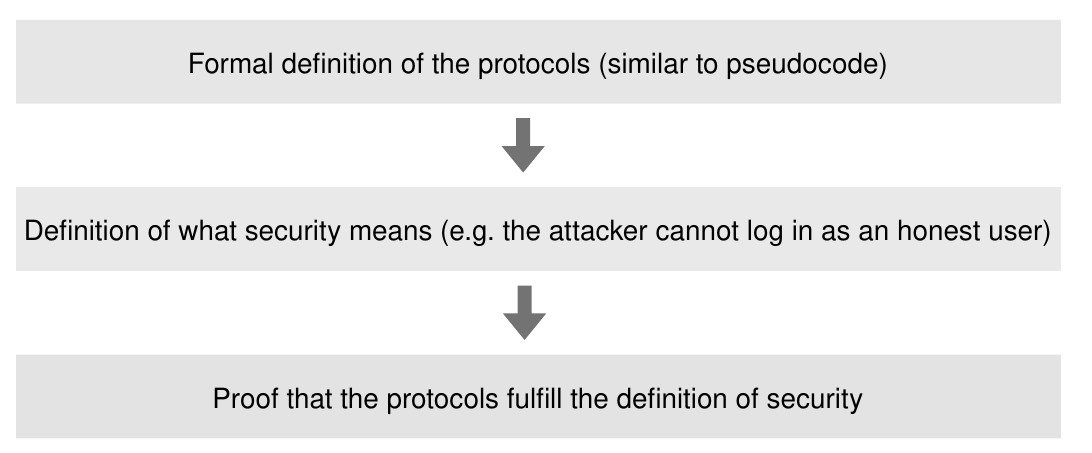
\includegraphics{images/png/formal-analysis-steps.png}}

    \fonte{\citeonline{hauck2023openid}}
    \label{fig:formal-analysis-steps}
\end{figure}


Para ilustrar o funcionamento desse tipo de análise, será reproduzida uma parte da Prova de Autenticação de Apresentação (Presentation Authentication) conforme descrita em \cite{hauck2023openid}. O objetivo deste capítulo não é fornecer uma explicação detalhada e exaustiva da prova, mas sim uma compreensão intuitiva do processo de análise. Este capítulo é, portanto, dividido em três subseções. Na \autoref{subsection:formal-definition-using-win}, será apresentado \sigla{WIM}{Web Infrastructure Model} utilizado como base para definir formalmente o \acs{OIDC4VP}, em um formato similar a pseudo-código. Na \autoref{subsection:properties-of-formal-analysis} será especificado o significado da Autenticação de Apresentação neste contexto, e, finalmente, na \autoref{subsection:proof-of-formal-analysis}, será apresentada a prova.

\subsection{Definição Formal de Protocolos Usando WIM}\label{subsection:formal-definition-using-win}

O modelo \acs{WIM} segue uma abordagem baseada no modelo \sigla{DV}{Dolev-Yao}, capturando padrões web amplamente utilizados, como HTTP e HTML. A \autoref{fig:wim-model} ilustra a arquitetura do modelo. Nele, cada entidade é representada por um processo que monitora um ou mais endereços IP e processa eventos correspondentes. Um evento é composto por uma mensagem e pelos endereços IP do remetente e do destinatário. Em cada etapa de processamento, um evento é selecionado de maneira não determinística de uma lista de eventos e entregue ao processo apropriado. A entidade processa o evento e gera um ou mais novos eventos, que são, então, adicionados à lista para processamento subsequente \cite{fett2024wim}.

Para modelar o \acs{OIDC4VP}, o comportamento do atacante e do navegador web são especificados como processos. 
O processo do atacante é um processo Dolev-Yao não determinístico que registra todas as mensagens que recebe e gera todos os eventos que pode derivar das mensagens registradas. 
Mais formalmente, um processo atacante $(I, Z, R, s_0)$ que recebe um evento de entrada $e_{in}$ em um estado $s$ gera o novo estado $s' = \langle e_{in}, E_{out}, s \rangle$ e os eventos 
$E_{out} = \{ \langle a_1, f_1, m_1 \rangle, \ldots, \langle a_n, f_n, m_n \rangle \}$ 
para algum $n \geq 0$, onde os endereços do remetente $f_1, \ldots, f_n$ são escolhidos de forma não determinística a partir de $I$, os endereços do destinatário $a_1, \ldots, a_n$ são escolhidos não deterministicamente entre todos os endereços IP, e as mensagens $m_1, \ldots, m_n$ são escolhidas não deterministicamente de $d(\{e_{in}\} \cup \{s\})$ \cite[Seção 2.5]{FettKS14}.
Dessa forma, um processo atacante é capaz de realizar todos os ataques que qualquer processo Dolev-Yao poderia executar, exceto quebrar criptografia.

Nesta análise, utiliza-se o modelo de atacante de rede, que tem acesso a todos os endereços IP, permitindo-lhe interceptar mensagens destinadas a outras partes e falsificar os endereços dos remetentes. Em redes reais, esses ataques podem incluir ARP-spoofing, onde o atacante redireciona tráfego em redes locais ao falsificar a correspondência entre endereços IP e endereços MAC, e ações de adversários patrocinados por estados-nação, que exploram infraestrutura de telecomunicação para interceptar e manipular dados em larga escala.

O atacante pode, ainda, corromper qualquer processo legítimo, ganhando acesso completo ao estado da entidade comprometida.
Isso é representado pelo envio de uma mensagem especial, $m = \text{CORRUPT}$, ao processo correspondente \cite[Seção 2.5]{FettKS14}. Após receber essa mensagem, o processo começa a atuar como um processo atacante, utilizando o último estado disponível. Os detalhes sobre como ocorre a corrupção variam de acordo com o modelo específico do processo.


O navegador web faz parte de um sistema que formaliza a infraestrutura da web e suas aplicações associadas. Para simplificar o modelo, o \acs{WIM} inclui um servidor HTTPS genérico, responsável, entre outras funções, por receber e enviar requisições HTTPS.

\begin{figure}[htb]
    \caption{Modelo WIM}
    \centering
    \resizebox{\linewidth}{!}{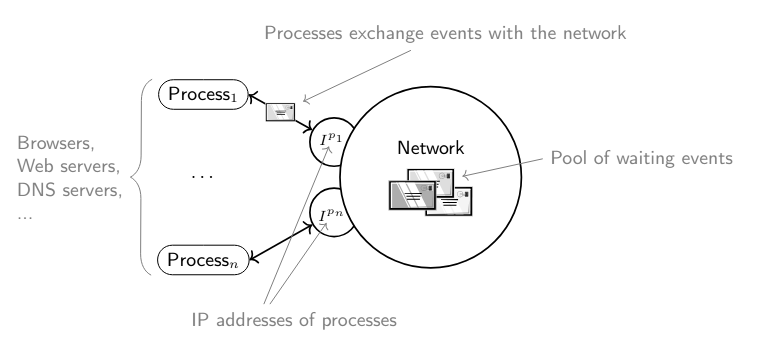
\includegraphics{images/png/wim-model.png}}
    \label{fig:wim-model}
    \fonte{\cite{fett2024wim}}
\end{figure}

\subsection{Propriedades de segurança}\label{subsection:properties-of-formal-analysis}


Uma etapa crucial para a comprovação de segurança é definir o que ela significa em um contexto específico, o que se faz por meio da identificação das propriedades de segurança relevantes. No caso do \acs{OIDC4VP}, uma dessas propriedades é a \textbf{Autenticação de Apresentação} (Presentation Authentication), que garante que um atacante não consiga se passar por um usuário legítimo para acessar uma aplicação. Em um ambiente web, essa propriedade é comprometida se um atacante obtiver posse de um cookie de sessão associado a um ID de usuário legítimo.

\subsection{Prova de segurança}\label{subsection:proof-of-formal-analysis}

% ---------------------- DECISÃO DE EXPLICAÇÃO ----------------------------------%
% - Não vou falar do response_mode direct_post. Teria que explicar mais um fluxo, e não acrescenta nada na proposta. Seria apenas ilustrativo para mostrar como a prova funciona.
% - Estou desconsiderando (Same-device e Cross-device flow), pois ao meu ver os tipos de ataques (Conseguir a apresentação e conseguir o session ID autorizado), servem tanto para um quanto para outro
% ---------------------- DECISÃO DE EXPLICAÇÃO ----------------------------------%

Para demonstrar a segurança da Autenticação de Apresentação, são estabelecidas duas premissas: (1) o usuário é perfeito, ou seja, ele sempre mantém o controle de quais fluxos iniciou; e (2) as entidades Browser, Carteira e Verificador são honestas, ou seja, não divulgam informações. Com base nessas premissas, deve-se provar que o atacante não consegue obter um cookie de sessão vinculado à identidade de um usuário legítimo. Isso ocorre porque as sessões são tipicamente identificadas por um nonce armazenado no navegador do usuário como um cookie. Se um atacante obtiver acesso a esse cookie, ele pode se passar pelo usuário legítimo, reutilizando o cookie comprometido para acessar a sessão ativa no sistema e, assim, obter os mesmos privilégios e acessos que o usuário original.

O cookie é gerado apenas no endpoint de redirecionamento (redirect endpoint), onde o verificador recebe a resposta de autorização (Authorization Response). Para que o atacante obtenha esse cookie, existem duas opções: a primeira seria que uma das partes honestas vazasse o cookie de sessão, o que é prevenido pela premissa (2); a segunda seria o atacante conseguir utilizar o redirect endpoint do verificador com sucesso. No entanto, isso só pode ser feito por meio de uma resposta de autorização contendo um \textbf{\texttt{redirect\_uri}}.


% \newtheorem{premise}{Premissa}
% \begin{premise}
%     \textbf{O usuário é perfeito}\label{premise:perfect-user}: O usuário sempre mantém o controle de quais fluxos ele iniciou.
% \end{premise}

% \begin{premise}
%     \textbf{As entidades Browser, Carteira e Verificador são honestas}\label{premise:honest-entity}: Entidades que não divulgam informações.
% \end{premise}

Para que o atacante obtenha um \textbf{\texttt{redirect\_uri}} com a identidade de um usuário legítimo, a possibilidade de uma entidade honesta divulgá-lo é descartada, conforme descrito em (1). Além disso, o atacante poderia tentar acessar a chave privada associada à chave pública da credencial do usuário, o que também é impedido pela \textbf{Propriedade de Emissão Autenticada}, detalhada em \cite{hauck2023openid}. Outra opção seria induzir uma carteira legítima a criar um \textbf{\texttt{redirect\_uri}} arbitrário.

Uma das táticas que o atacante pode usar para induzir uma carteira a gerar um \textbf{\texttt{redirect\_uri}} envolve o uso de um ataque de phishing. Nesse cenário, o atacante engana o usuário para que ele clique em um link ou visite uma página maliciosa, desencadeando involuntariamente um processo de autenticação com sua carteira digital. Durante esse processo, a carteira recebe uma requisição de autorização com o parâmetro \textbf{\texttt{redirect\_uri}} direcionado para um domínio controlado pelo atacante. No entanto, ao obter o \textbf{\texttt{redirect\_uri}}, o atacante não consegue utilizá-lo, pois o parâmetro \textbf{aud} (audience) é preenchido com o domínio do \textbf{\texttt{redirect\_uri}}, tornando o ataque ineficaz.


% ---------------------- DECISÃO DE EXPLICAÇÃO ----------------------------------%
% - Esse fluxo só acontece no response_mode direct_post. 
% ---------------------- DECISÃO DE EXPLICAÇÃO ----------------------------------%
% Um segundo cenário de ataque ocorre quando o atacante obtém conhecimento de um ID de Sessão previamente autenticado. Para que isso aconteça, seria necessário violar a(\autoref{premise:honest-entity}), que é uma garantia de segurança. No entanto, o atacante ainda pode tentar enganar o usuário. Nesse cenário, o atacante pode criar um ID de Sessão com um verificador e fazer o usuário enviar uma apresentação com as suas credenciais para a sessão iniciada pelo atacante. Isso não ocorrerá, desde que o usuário esteja ciente dos seus fluxos, como descrito pela garantia \autoref{premise:perfect-user}.

\begin{figure}[htb]
    \caption{Prova de Autenticação da Apresentação}
    \centering
    \resizebox{\linewidth}{!}{
        \begin{tikzpicture}[
    node distance=2cm and 3cm,
    every node/.style={draw, rectangle, align=center, text width=5cm, minimum height=2cm},
    arrow/.style={draw, -{Latex[width=2mm]}, thick}
    ]
    
    % Nodes
    \node (l1) {O atacante obtém o token de serviço};
    
    \node (l2-1) [below left=of l1] {O atacante consegue chamar o redirect\_endpoint com sucesso.};
    \node (l2-2) [below right=of l1] {Token de serviço é divulgado por meio de uma entidade honesta};
    
    \node (l3-1) [below left=of l2-1] {Atacante obtém um vp\_token válido};
    % \node (l3-2) [below right=of l2-1] {Atacante conhece um ID de sessão autorizada};
    \node (l3-3) [below=of l2-2, fill=gray!20] {\textbf{Falso}\\em virtude da Premissa 1};
    
    \node (l4-1) [below left=of l3-1] {O vp\_token é divulgado para o atacante};
    \node (l4-2) [below=of l3-1] {O atacante induz uma carteira legítima a gerar um vp\_token em seu nome, permitindo que ele o envie para um verificador.};
    \node (l4-3) [below right=of l3-1] {Atacante sabe a chave privada da credencial do usuário legítimo};
    % \node (l4-4) [below=of l3-2] {O atacante cria seu próprio ID de sessão com o verificador};
    % \node (l4-5) [below right=of l3-2] {ID de Sessão é divulgado};
    
    \node (l5-1) [below=of l4-1, fill=gray!20] {\textbf{Falso}\\em virtude da Premissa 1};
    % ---------------------- EXPLICAÇÃO ----------------------------------%
    % -- Existe a possibilidade de não alterar o redirect\_uri. Porém o atacante teria que:
    % -- 1. Fazer um script para iniciar a sessão com um verificador (Ter um ID de Sessão para o usuário mas que o atacante tenha acesso?)
    % -- 2.1 Atacante pode interceptar a resposta, mas está criptografada.
    % -- 2.2 A resposta chega e redireciona o usuário para o redirec_uri definido previamente (fluxo normal seguro)
    % -- OU
    % -- 1. O Atacante inicia uma sessão com um verificador fora do browser do usuário
    % -- 2. Engana o usuário (com um script no browser dele) para enviar o vp_token para o verificador que o atacante tem um ID de Sessão.
    % -- 3. Verificador recebe o vp_token, mas dá erro porque vem com a origem do usuário a qual não têm sessão com ele.
    % ---------------------- EXPLICAÇÃO ----------------------------------%
    \node (l5-2) [below=of l4-2] {O atacante tenta modificar a Requisição de Autorização enviada à carteira, alterando o \textbf{redirect\_uri} para um domínio sob seu controle, com o objetivo de redirecionar a resposta para um verificador legítimo e se passar pelo usuário que solicitou a apresentação.};
    \node (l5-3) [below=of l4-3, fill=gray!50] {\textbf{Falso}\\Quebra a Propriedade de segurança da autenticação de emissão};
    % \node (l5-4) [below=of l4-4] {A requisição de autorização é enviada ao usuário através de phishing};
    % \node (l5-5) [below=of l4-5, fill=gray!20] {\textbf{Falso}\\em virtude da Premissa 1};
    

    % ---------------------- EXPLICAÇÃO ----------------------------------%
    % - O nodo abaixo pode parecer incompleto, ou mal explicado, mas a jutificativa está diretamente relacionada com a proposta de algoritmo que está descrita no texto.


  
    % ----------------------  EXPLICAÇÃO ----------------------------------%
    \node (l6-1) [below=of l5-2, fill=gray!20]  {\textbf{Falso}\\O atacante não consegue gerar um vp\_token válido, pois o campo \textbf{aud} utiliza o domínio do \textbf{redirect\_uri} como valor, tornando-o inválido e inutilizável.};

    % \node (l6-2) [below=of l5-4, fill=gray!20] {\textbf{Falso}\\em virtude da Premissa 2};
    
    % Connections
    \draw[arrow] (l1) -- (l2-1);
    \draw[arrow] (l1) -- (l2-2);
    \draw[arrow] (l2-1) -- (l3-1);
    % \draw[arrow] (l2-1) -- (l3-2);
    \draw[arrow] (l2-2) -- (l3-3);
    \draw[arrow] (l3-1) -- (l4-1);
    \draw[arrow] (l3-1) -- (l4-2);
    \draw[arrow] (l3-1) -- (l4-3);
    % \draw[arrow] (l3-2) -- (l4-4);
    % \draw[arrow] (l3-2) -- (l4-5);
    \draw[arrow] (l4-1) -- (l5-1);
    \draw[arrow] (l4-2) -- (l5-2);
    \draw[arrow] (l4-3) -- (l5-3);
    % \draw[arrow] (l4-4) -- (l5-4);
    % \draw[arrow] (l4-5) -- (l5-5);
    % \draw[arrow] (l5-4) -- (l6-2);
    

    \draw[arrow] (l5-2) -- (l6-1);
   
    
\end{tikzpicture}

    }
    \fonte{O Autor}
    \label{fig:proof-of-presentation-authentication}
\end{figure}
\chapter{Trabalhos relacionados}

\section{\sigla{OPAL}{Open Algorithms}}

O Open Algorithms (OPAL) é uma iniciativa do MIT Media Lab que visa permitir o uso de dados sensíveis e pessoais para análises, assegurando ao mesmo tempo a privacidade dos indivíduos. O projeto adota alguns princípios fundamentais dentro do seu modelo, como o de deslocar os algoritmos para os dados. Este princípio sugere que, em vez de transferir dados de vários repositórios para um local centralizado para processamento, os algoritmos devem ser direcionados aos repositórios de dados para serem processados localmente. Dessa forma, busca-se garantir que informações pessoais não sejam transferidas em seu formato bruto, mas apenas as análises e percepções (insights) derivadas desses dados. Esse método preserva a privacidade ao permitir que apenas resultados agregados sejam retornados após a execução dos algoritmos.

Para que isso ocorra, um dos principais conceitos introduzidos para o tratamento de dados é o de \textbf{Algoritmos Verificados} (Vetted Algorithms). Este conceito estabelece que os algoritmos utilizados no ecossistema são previamente revisados e aprovados por especialistas, conhecidos como \textbf{Autoridade Verificadora} (Vetting Authority), que centralizam a decisão sobre quais algoritmos devem ou não ser empregados. Essa abordagem visa, sobretudo, assegurar a qualidade dos algoritmos sob a perspectiva de viés, injustiça, e outros possíveis efeitos colaterais não intencionais ou imprevistos.

Outro aspecto importante abordado é o atual isolamento dos dados. Sugere-se que percepções mais aprofundadas podem ser alcançadas quando há uma integração de dados de diferentes domínios — como dados de saúde, financeiros, redes sociais, etc. A ideia é que, ao combinar e analisar esses dados em conjunto, torna-se possível identificar padrões, correlações e tendências que não seriam detectáveis ao se considerar apenas um único conjunto de dados. Por exemplo, ao combinar dados de compra provenientes de diferentes lojas e bancos, as empresas podem obter uma compreensão mais abrangente dos comportamentos de consumo, o que permite a implementação de campanhas de marketing mais eficazes e personalizadas.


A concepção geral desse ecossistema é estabelecer dois atores principais: o \textbf{Provedor de Dados} (Data Provider) e o \textbf{Serviço de Dados \acs{OPAL}} (OPAL Data Service), que podem ser a mesma entidade ou entidades distintas. A interação entre esses atores e outras entidades é representada na \autoref{fig:opal-ecossytem}. O Consultor, geralmente representado como \acs{SP} em aplicações web, que deseja obter informações, utiliza a Aplicação no Passo 1 para selecionar um ou mais algoritmos e os dados desejados (Passo 2). Em seguida, o Consultor usa a Aplicação para transmitir essas seleções ao Serviço de Dados, também chamado de OPAL Gateway, no Passo 3. O Serviço de Dados, então, interage com os Provedores de Dados relevantes no Passo 4 para executar a solicitação. Finalmente, o Serviço de Dados envia a resposta para a Aplicação e o Consultor no Passo 5.

\begin{figure}[h]
    \caption{Ecossistema \acs{OPAL}.}
    \centering    
    \resizebox{\linewidth}{!}{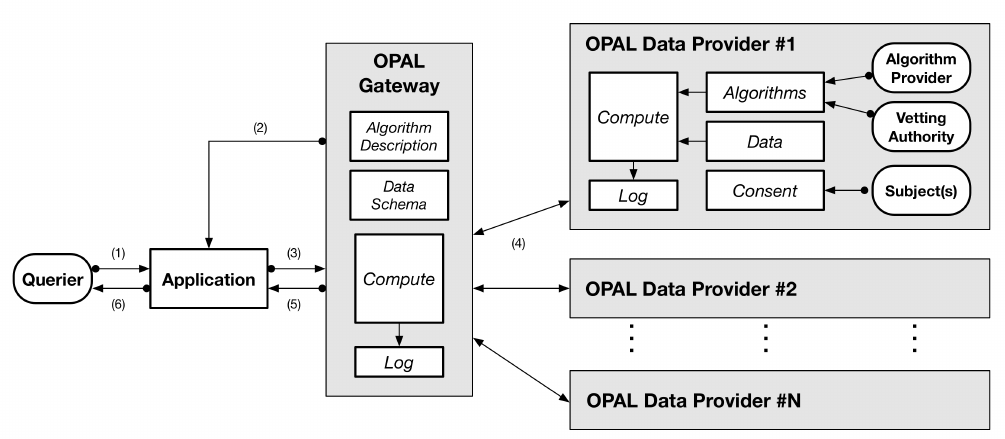
\includegraphics{images/png/OPAL-ecossytem.png}}
    \fonte{\citeonline{opal}}
    \label{fig:opal-ecossytem}
\end{figure}


\section{Machine Readable Personal Privacy Terms}

\sigla{MRPTWG}{Machine Readable Privacy Terms Working Group} é um grupo de trabalho da IEEE que está desenvolvendo o padrão Machine Readable Personal Privacy Terms. 
Apesar de ainda não ter nenhuma publicação, o objetivo descrito em seu resumo é tratar de como os termos de privacidade pessoal são estruturados, buscando possibilitar que sejam compreendidos e aceitos por máquinas.
Essa abordagem permitiria que dispositivos e sistemas em uma rede concordassem de maneira clara e precisa sobre a divulgação e o uso de informações. A relevância e o impacto desse padrão dependem, evidentemente, de sua implementação prática, o que o torna um tópico de interesse significativo para a evolução das políticas de privacidade digital. Portanto, merece ser mencionado aqui.

\section{Comparação entre propostas}

\begin{table}[h]
  \caption{Comparação entre Propostas}
  \label{tab:related}
  \resizebox{\textwidth}{!}{%
  \begin{tabular}{@{}lcccc@{}}
  \toprule
  \textbf{\color[HTML]{000000} Proposta}                                           & \textbf{\begin{tabular}[c]{@{}l@{}}Nível de\\ Atuação\end{tabular}}             & \textbf{\begin{tabular}[c]{@{}l@{}}Ambiente de\\ Execução\end{tabular}}           & \textbf{\begin{tabular}[c]{@{}l@{}}Dados\\ Compartilhados\end{tabular}}            & \textbf{\begin{tabular}[c]{@{}l@{}}Algoritmos\\ Verificados\end{tabular}}            \\ \midrule
  
  OPAL                                                                             & Modelo                                                                         & \begin{tabular}[c]{@{}c@{}}Provedor de \\ Dados\end{tabular}                       & sim                                                                                & sim                                                                                  \\ \midrule

  \begin{tabular}[c]{@{}l@{}}Machine Readable Personal Privacy Terms\end{tabular} & Padrão                                                                          & \begin{tabular}[c]{@{}c@{}}Sem informações\end{tabular}                            & Sem informações                                                                    & Sem informações                                                                      \\ \midrule 
  \begin{tabular}[c]{@{}l@{}}Novo Protocolo para \\ Modelo Fiduciário\end{tabular} & Protocolo                                                                      & \begin{tabular}[c]{@{}c@{}}SP, Fiduciário ou\\ ambos\end{tabular}                  & não                                                                                & não                                                                                  \\ \bottomrule
  \end{tabular}%
  }
  \fonte{O Autor}
  \end{table}
  

A \autoref{tab:related} oferece uma comparação entre as duas propostas em relação a diferentes aspectos. Na coluna intitulada \textbf{Nível de Atuação}, observa-se a primeira grande diferença entre as propostas. 
Enquanto a \acs{OPAL} é descrita como um modelo, o \emph{Protocolo para Negociação de Atributos e Ambiente de Execução} é classificado como um protocolo. 
Essa distinção é crucial, pois destaca o objetivo principal de cada solução proposta. Em geral, um modelo está primariamente preocupado em descrever um ecossistema de forma abstrata, enfatizando seus princípios e fundamentos, ao invés de se concentrar em como implementar o modelo de maneira prática. Por outro lado, um protocolo aprofundará a descrição oferecida por um modelo, visando facilitar sua implementação prática.

Em termos de \textbf{Ambiente de Execução}, o \acs{OPAL} opera exclusivamente no Provedor de Dados, o que sugere uma mudança drástica em relação ao cenário atual. Por outro lado, o novo protocolo pode ser implementado no SP, no fiduciário ou em ambos, o que indica uma transição mais gradual para a execução de algoritmos em ambientes que oferecem maior confiança ao usuário. Na coluna \textbf{Dados Compartilhados}, o \acs{OPAL} possibilita o compartilhamento de dados, alinhando-se com práticas que promovem a colaboração. Em contraste, o novo protocolo não apresenta mecanismos específicos para o compartilhamento de dados. No entanto, o Modelo Fiduciário não impõe restrições a esse respeito, pois é viável que um fiduciário, com usuários de diferentes domínios, permita o compartilhamento de suas credenciais por meio de sua Política de Consentimento, visando adquirir novas análises sobre os dados.

Na coluna \textbf{Algoritmos Verificados}, o \acs{OPAL} também restringe seu escopo de atuação ao exigir, como princípio básico, a verificação de algoritmos. Essa exigência, por um lado, contribui para garantir a qualidade e a integridade das análises realizadas; por outro, pode atrasar o desenvolvimento de algoritmos mais atualizados e eficientes. Em contraste, o novo protocolo não incorpora nenhuma funcionalidade similar para a verificação de algoritmos, permitindo que o \acs{SP} apresente sua solução desejada, enquanto o fiduciário avalia se a proposta está de acordo com as definições de transparência e com as restrições impostas pelo seu beneficiário.





\chapter{Um Novo Protocolo Para Identidade Fiduciária}\label{ch:protocol}

O novo Protocolo para Identidade Fiduciária propõe uma modificação no protocolo \acs{OIDC4VP}, parte integrante do ecossistema \acs{OIDC4VC}, para adequá-lo ao Modelo Fiduciário. 
Através dessa adaptação facilitará a construção de uma camada de apresentação de credenciais de maneira simplificada, segura e amigável para os desenvolvedores. Destaca-se também a capacidade de reutilizar a infraestrutura existente, além do fácil acesso a uma vasta gama de códigos e bibliotecas desenvolvidas com base na especificação central do OpenID, o que amplifica sua adoção e integração. Essas características tornam o protocolo não apenas uma solução técnica eficiente, mas também uma abordagem estratégica que potencializa a escalabilidade e a interoperabilidade dentro do ecossistema de identidades digitais.

% % Pilha de protocolos 

% Além disso, a nova especificação introduz duas extensões que se alinham com as estratégias delineadas em \autoref{subsection:fiduciário} para a preservação da privacidade dos usuários: a Negociação de Atributos e a Negociação do Ambiente de Execução. A primeira utiliza a estrutura de \acs{DA}s em conjunto com a definição de novas mensagens e endpoints, visando à redução do risco de uso indevido de dados, garantindo que somente as informações estritamente necessárias sejam compartilhadas. De maneira similar, a segunda extensão, também baseada em  endpoints e mensagens, possibilita que dados e informações sensíveis sejam preferencialmente processados em ambientes confiáveis para o usuário. Essas inovações visam não apenas cumprir os requisitos de segurança, mas também aprimorar a confiança do usuário no sistema, ao assegurar que sua privacidade seja rigorosamente protegida em todas as etapas do processo.

% Dessa forma, este texto busca detalhar as adaptações requeridas no \acs{OIDC4VP} para garantir sua conformidade com a pilha especificada na \autoref{fig:stack-model-protocol-extension}, onde os protocolos e extensões são integrados para satisfazer as propriedades e comportamentos preconizados pelo Modelo Fiduciário. Essas adaptações asseguram o alinhamento com os princípios de privacidade estabelecidos por regulamentações como a \sigla{LGPD}{Lei Geral de Proteção de Dados}, representando um avanço significativo na evolução das identidades digitais, promovendo uma solução que equilibra inovação tecnológica com os mais altos padrões de proteção de dados.

% Assim, este texto tem como objetivo detalhar as adaptações necessárias no OIDC4VP para garantir sua conformidade com a pilha especificada na Figura 13. Essa pilha ilustra uma abordagem modular que pode ser utilizada para alcançar as propriedades e comportamentos previstos pelo Modelo Fiduciário. Embora o foco principal esteja na adaptação do \acs{OIDC4VP}, destacado em tons de cinza, deixa em aberto a viabilidade de explorar as demais soluções mencionadas em \autoref{subsec:oidc4vc}, representadas em branco, e adaptá-las para atender aos demais princípios previstos no modelo.

A nova especificação introduz duas extensões alinhadas às estratégias da \autoref{subsection:fiduciário} para a preservação da privacidade dos usuários: a \emph{Negociação de Atributos} e a \emph{Negociação do Ambiente de Execução}. A primeira utiliza a estrutura de \acs{DA}s em conjunto com a definição de novas mensagens e endpoints, visando à redução do risco de uso indevido de dados, garantindo que somente as informações estritamente necessárias sejam compartilhadas. Já a segunda extensão, também baseada em endpoints e mensagens, permite que dados sensíveis sejam preferencialmente processados em ambientes confiáveis ao usuário.

Essas adaptações são representadas na \autoref{fig:stack-model-protocol-extension}, que adota uma abordagem modular como solução para atingir as propriedades e comportamentos definidos pelo modelo. Embora o foco esteja no \acs{OIDC4VP}, destacado em tons de cinza, deixa-se em aberto a viabilidade de explorar as demais soluções mencionadas em \autoref{subsection:fiduciário}, representadas em branco, para atender aos demais princípios do modelo.
Essa solução visa não apenas cumprir os requisitos de segurança, mas também aprimorar a confiança do usuário no sistema, ao assegurar que sua privacidade seja rigorosamente protegida em todas as etapas do processo.

\begin{figure}[htb]
    \caption{Pilha: Modelo, protocolos, extensões.}
    \centering
    \resizebox{\linewidth}{!}{
        \begin{tikzpicture}[node distance=1cm,outer sep=1pt,inner sep=1pt]

    % CONFIGURANDO OS NODOS 
 
    %------------------------ CAMADA 3----------------------------%
    \tikzset{field/.style={align=center,shape=rectangle,rounded corners,minimum height=5cm,minimum width=20cm,draw,font=\fontsize{36}{44}\selectfont\sffamily,fill=gray!20}}

    \tikzset{field2/.style={align=center,shape=rectangle,rounded corners,minimum height=5cm,minimum width=29cm,draw,font=\fontsize{36}{44}\selectfont\sffamily,fill=gray!20}}

    %------------------------ CAMADA 2----------------------------%
    \tikzset{mediumfield/.style={align=center,shape=rectangle,rounded corners,minimum height=5cm,minimum width=40.5cm,draw,font=\fontsize{36}{44}\selectfont\sffamily,fill=gray!40}}

    \tikzset{mediumfield2/.style={align=center,shape=rectangle,rounded corners,minimum height=5cm,minimum width=14.5cm,draw,font=\fontsize{36}{44}\selectfont\sffamily,fill=gray!40}}

    \tikzset{mediumfield3/.style={align=center,shape=rectangle,rounded corners,minimum height=5cm,minimum width=13.9cm,draw,font=\fontsize{36}{44}\selectfont\sffamily,fill=gray!40}}

 %------------------------ CAMADA 1----------------------------%
    \tikzset{largefield/.style={align=center,shape=rectangle,rounded corners,minimum height=5cm,minimum width=70cm,draw,font=\fontsize{36}{44}\selectfont\sffamily,fill=gray!40}}


    % INSTANCIANDO OS NODOS
    
    %------------------------ CAMADA 1----------------------------%
    % Desenho do primeiro retângulo (grande)
    \node [largefield] (fid) {Modelo Fiduciário};


    %------------------------ CAMADA 2----------------------------%
    % Desenho do segundo retângulo (médio), alinhado à direita com o primeiro, e posicionado acima
    \node [mediumfield,anchor=south east] at ([yshift=0.5cm]fid.north east) (oidc4vp) {OIDC4VP};

     % Desenho do segundo retângulo (médio), alinhado à direita com o primeiro, e posicionado acima
    \node [mediumfield2,anchor=south east, fill=white] at ([xshift=-0.5cm]oidc4vp.south west) (oidc4ci) {OIDC4CI};

    \node [mediumfield3,anchor=south east, fill=white] at ([xshift=-0.5cm]oidc4ci.south west) (siopv2) {SIOPv2};
    %------------------------ CAMADA 3----------------------------%

    \node [field,anchor=south east] at ([yshift=0.5cm]oidc4vp.north east) (atributes) {Negociação de Atributos};
    
    \node [field,anchor=south east] at ([xshift=-0.5cm]atributes.south west) (env) {Negociação de \\ Ambiente de Execução};

    % \node [mediumfield2,anchor=south east, fill=white, minimum width=14cm] at ([xshift=-0.5cm]env.south west) (ext1) {Extensão 1};
    \node [mediumfield2,anchor=south east, fill=white, minimum width=14.5cm] at ([xshift=-0.5cm]env.south west)  (ext1) {Extensão 1};
    \node [mediumfield2,anchor=south east, fill=white, minimum width=2cm, draw=white] at ([xshift=-0.5cm]ext1.south west) (dots) {...};
    \node [mediumfield2,anchor=south east, fill=white, minimum width=11.2cm] at ([xshift=-0.5cm]dots.south west) (extn) {Extensão n};    

    % \node [mediumfield2,anchor=south east, fill=white, draw=white] at ([xshift=-0.5cm]ext1.south west) (env) {\large{...}};
    % \node [field2,anchor=south east] at ([xshift=-0.5cm]env.south west) (aud) {Auditoria};
    
    
    
\end{tikzpicture}
    }
    \fonte{O Autor}
    \label{fig:stack-model-protocol-extension}
\end{figure}

\section{Integração do OIDC4VP com o Modelo Fiduciário}

A transição do modelo original de \acs{SSI}, no qual o \acs{OIDC4VP} foi originalmente proposto, para o Modelo Fiduciário, é um processo bastante natural como mostrado na \autoref{fig:oidc4vp-in-fid}. 
Isso ocorre porque esta adaptação foca exclusivamente na redução da divulgação de dados proposto por \emph{Non-Disclousure as Goal}, sem exigir, por exemplo, modificações nas mensagens trocadas pelo Fiduciário como solução para garantir maior controle sobre as ações realizadas com os dados do usuário, conforme previsto no princípio de \emph{Transparency for Accountability}.
Dessa forma, não foram necessárias alterações significativas, permitindo que a \acs{SP} continue desempenhando seu papel como a entidade responsável por solicitar, receber e validar as \acs{VP}s. No contexto do \acs{OIDC4VP}, essa função é exercida por meio do papel de Cliente OAuth.

O Fiduciário, por sua vez, possui as mesmas funções e capacidades que a Carteira, conforme discutido anteriormente na \autoref{subsection:fiduciário}, incluindo receber, armazenar, apresentar e gerenciar as \acs{VC}s, bem como as chaves criptográficas associadas. Portanto, no contexto do \acs{OIDC4VP}, deve assumir o papel Servidor de Autorização que é realizado pela Carteira dentro desse contexto. No entanto, com a prioridade de, além de adquirir um mecanismo para entregar \acs{VP}s, integrar as extensões de \emph{Negociação de Atributos} e \emph{Negociação do Ambiente de Execução} nos fluxos existentes, visando atender o pilar \emph{Non-Disclosure as Goal}.
% Mudanças em oidc4vp
\begin{figure}[htb]
    \caption{Fluxo com Fiduciário no lugar da Carteira.}
    \centering
    \resizebox{\linewidth}{!}{\begin{sequencediagram}[scale=0.1]
    \newthread{A}{\ttfamily Usuário}{}
    \newinst[4]{C}{\ttfamily Fiduciário}{}
    \newinst[11]{B}{\ttfamily \acs{SP}}{}
    
    \newcounter{number}
    \stepcounter{number}
    \begin{call}{A}{\ttfamily Interação}{B}
        \postlevel
        \postlevel
        \postlevel
        \stepcounter{number}
            \begin{call}{B}{\shortstack{ \ttfamily (1) Requisição de Autorização \\ \ttfamily (client\_id, nonce, redirect\_uri, presentation\_definition)}}{C}{\shortstack{\ttfamily (2) Resposta de Autorização \\ \ttfamily (vp\_token, presenation\_submission)}}
            \postlevel
            \postlevel

            % Adicionando uma nota após o passo 1
            \node at (1.5,-4) [text width=6cm, anchor=west] {\ttfamily \small Autenticação e Confirmação/Seleção da \acs{VC}};

            \postlevel
            
        \end{call}
    \end{call}
\end{sequencediagram}}
    \label{fig:oidc4vp-in-fid}
    \fonte{O Autor}
\end{figure}

\section{Uso de Provas de Conhecimento Zero}

A utilização da especificação OIDC4VP no Modelo Fiduciário visa aproveitar a flexibilidade e a concepção agnóstica em relação ao formato das Credenciais Verificáveis utilizadas. Isso significa que sua adaptação ao modelo não exige diretamente o uso de Provas de Conhecimento Zero; ao contrário, proporciona um ambiente que permite a integração de \acs{VC}s que possuam essa capacidade. Como o \acs{OIDC4VP} não estabelece requisitos específicos para a implementação de \acs{ZKP}, cabe aos formatos de \acs{VC}s adotados determinar se oferecem suporte ou não para essa tecnologia. O uso dessa tecnologia é recomendado especialmente em contextos que exigem altos níveis de privacidade e segurança na verificação das credenciais, permitindo que apenas as informações estritamente necessárias sejam divulgadas.

\section{Negociação de Atributos}\label{section:attribute-negotiation}

Quando um Fiduciário recebe uma Requisição de Autorização é possível que a Definição de Apresentação solicite informações do usuário as quais não estejam de acordo com as Políticas de Consentimento definidas previamente. Por exemplo, é comum que Provedores de Serviço realizem a solicitação da data de nascimento dos  usuários apenas para verificar sua maioridade. Este tipo de requisição é invasiva e pode estar contra os desejos do indivíduo. Dessa forma, a extensão \textbf{Negociação de Atributos} permite definir quais informações sobre os usuários são relevantes para a plataforma que está oferecendo serviços sem comprometer a privacidade e o sigilo dos dados do dono desses recursos.

Esse mecanismo está centrado na estrutura de \acs{DA}s, que no modelo Fiduciário são chamados de \textbf{Declarações de Requisitos} (Requirements Statements). Neste texto, os termos \acs{DA}s e Declarações de Requisitos serão tratados como sinônimos. Com essa estrutura, os Fiduciários conseguem definir quais informações requisitadas não estão em conformidade com as Políticas de Consentimento e propor novos que satisfaçam as intenções. Para que isso seja possível, são definidos o endpoint Negociação (Negotiation Endpoint), a Solicitação de Negociação (Negotiation Request) e sua respectiva resposta, Resposta de Negociação (Negotiation Response). 
Essa nova requisição, iniciada pelo Fiduciário e respondida pelo \acs{SP}, ocorre entre a Requisição de Autorização e sua respectiva resposta, conforme destacado na \autoref{fig:attribute-negotiation-flow-via-browser}.

\begin{figure}[htb]
    \caption{Fluxo para Negociação de Atributos}
    \centering
    \resizebox{\linewidth}{!}{\begin{sequencediagram}[scale=0.1]
    \newthread{A}{\ttfamily Navegador}{}
    \newinst[6]{B}{\ttfamily Fiduciário}{}
    \newinst[15]{C}{\ttfamily \acs{SP}}{}
    
    \begin{call}{A}{\ttfamily Interação}{C}
        \postlevel
        \postlevel
        \postlevel
            \begin{call}{C}{\shortstack{ \ttfamily (1) Requisição de Autorização \\ \ttfamily (client\_id, nonce, redirect\_uri, presentation\_definition, client\_metadata)}}{A}{\shortstack{\ttfamily (2) Resposta de Autorização \\ \ttfamily (vp\_token, presenation\_submission)}}
            \postlevel
            \postlevel

            \begin{call}{A}{\shortstack{ \ttfamily (1) Requisição de Autorização}}{B}{\shortstack{\ttfamily (2) Resposta de Autorização}}

                \postlevel
                \postlevel
                % Adicionando uma nota após o passo 1
                % \node at (1.5,-4) [text width=6cm, anchor=west] {\ttfamily \small Autenticação e Confirmação/Seleção da \acs{VC}};
    
                \postlevel
                \begin{call}{B}{\shortstack{ \ttfamily Requisição de Negociação\\ \ttfamily (type, definition\_id, presentation\_definition)}}{C}{\shortstack{ \ttfamily Resposta de Negociação\\ \ttfamily(status)}}
                \postlevel
                \end{call}

            \postlevel  
            \end{call}

            \postlevel
            \postlevel
            
        \end{call}
    \end{call}
\end{sequencediagram}

}
    \fonte{O Autor}
    \label{fig:attribute-negotiation-flow-via-browser}
\end{figure}


\subsection{Endpoint de Negociação}\label{subsection:endpoint-negociação}

Este endpoint é utilizado para negociar Declaração de Requisitos previamente encaminhada em casos os quais o Fiduciário identifica alguma divergência do que foi requisitado e o que é autorizado dentro das Políticas de Consentimento. A comunicação com o Endpoint de Neogicação deve utilizar TLS.

Para o Fiduciário obter o \emph{Endpoint de Negociação} do Provedor de Serviços, este texto define o parâmetro \texttt{negotiation\_endpoint}, que pode ser adquirido por dois meios. O primeiro é pelo mecanismo tradicional de registro \acs{OIDC-D} de \cite{sakimura2023openidDiscovery}, no qual os Clientes OAuth fornecem seus metadados aos Servidores de Autorização. O segundo é por meio do parâmetro \texttt{client\_metadata}, conforme definido na seção 5 \cite{OIDC4VP2023}, enviado na Requisição de Autorização e contendo os metadados do \acs{SP}.

\begin{itemize}
    \item \textbf{negotiation\_endpoint}: URL do Endpoint de Negociação do Provedor de Serviços. Esta URL deve usar o esquema HTTPS e pode conter componentes de porta, caminho e parâmetros de consulta. Se omitido, o provedor não oferece suporte a esse endpoint e não está em conformidade com as propriedades do Modelo Fiduciário.
\end{itemize}

% Endpoint de Negocição
\begin{figure}[htb]
    \caption{Exemplo de parâmetro negotiation\_enpoint no client\_metadata (em UTF-8)}
    \centering
    \input{code/json}


% Exemplo baseado na Seção 5 (Authorization Request) do OIDC4VP
\begin{lstlisting}[language=json,firstnumber=1]
GET /authorize?
  client_id=client.example.org
  &client_metadata=%7B%22vp_formats%22%3A%7B%22jwt_vp_json%22%3A%7B%22alg%22%3A%5B%22EdDSA%22%2C%22ES256K%22%5D%7D%7D%2C%22negotiation_endpoint%22%3A%22https%3A%2F%2Fexample.com%22%7D
  &request_uri=https%3A%2F%2Fclient.example.org%2Frequest%2Fvapof4ql2i7m41m68uep
  &request_uri_method=post HTTP/1.1
\end{lstlisting}
    \fonte{O Autor}
    \label{fig:negotiation-endpoint}
\end{figure}

\subsection{Solicitação de Negociação}\label{subsection:negotiation-request}

A Solicitação de Negociação constitui uma requisição HTTP POST enviada pelo Fiduciário ao \acs{SP}, com o tipo de mídia \texttt{application/json}. Os parâmetros utilizados na solicitação são os seguintes:

% Requisição de Negociação
\begin{figure}[htb]
    \caption{Solicitação de Negociação}
    \centering
    \input{code/json}

\begin{lstlisting}[language=json,firstnumber=1]
POST /negotiate HTTP/1.1
Host: example.com
Content-Type: application/json

{
  "type": "attribute",
  "definition_id": "8xLOxBtZp8",
  "presentation_definition": "..."
}
\end{lstlisting}
    \fonte{O Autor}
    \label{fig:negotiation-request}
\end{figure}

\begin{itemize}

    \item \textbf{type}: OBRIGATÓRIO. Este parâmetro deve ser utilizado na Solicitação de Negociação para especificar o tipo de negociação que está sendo realizada. No contexto da \emph{Negociação de Atributos}, deve-se utilizar o valor \texttt{attribute}.

    \item \textbf{definition\_id}: OPCIONAL. Trata-se de uma string que identifica uma Declaração de Requisitos previamente encaminhada ao Fiduciário. Após o acordo ser firmado entre o Fiduciário e o Provedor, o \acs{SP} deve invalidar o \texttt{definition\_id}. Este parâmetro se torna OBRIGATÓRIO quando o valor de \texttt{type} é \texttt{attribute}.
    
    \item \textbf{presentation\_definition}: OPCIONAL. Este parâmetro contém um objeto JSON de Declaração de Requisitos, conforme a sintaxe estabelecida na \cite{presentation-exchange}. Este parâmetro se torna OBRIGATÓRIO quando o valor de \texttt{type} é \texttt{attribute}.
    
\end{itemize}

\subsection{Resposta de Negociação}

O Provedor de Serviços possui a prerrogativa de aceitar ou recusar a proposta de alteração da Declaração de Requisitos. Em determinados casos, o Fiduciário aceita a proposta que contém a nova Declaração de Requisitos e responde com uma mensagem com tipo de mídia \texttt{application/json} contendo em seu corpo o \acs{JSON} com o parâmetro status indicando a aceitação da sugestão de declaração e o código de status HTTP 202 sinalizando está pronto para receber a nova declaração, que é diferente daquele que o \acs{SP} enviou em sua Requsição de Autorização. 

% % Resposta de Negocição bem sucedida
\begin{figure}[htb]
    \caption{Resposta de Negociação com Sucesso.}
    \centering
    \input{code/json}

\begin{lstlisting}[language=json,firstnumber=1]
HTTP/1.1 201 Accepted
Content-Type: application/json

{
    "status": "accepted"
}

\end{lstlisting}
    \fonte{O Autor}
    \label{fig:negotiation-response-success}
\end{figure}

\begin{itemize}
    
   \item \textbf{status}: OBRIGATÓRIO. A semântica desse campo irá depender da negociação definida em type. Nesse exemplo, indica se o \acs{SP} aceitou ou recusou a nova proposta para a Declaração de Requisitos. O código de status em formato ASCII selecionado entre as duas opções abaixo:

    \begin{itemize}
        \item \textbf{accepted}: Indica que a proposta para a nova Declaração de Requisitos foi aceita pelo \acs{SP}. Nesse caso, o processo de alteração da Declaração de Requisitos será iniciado, e o recurso associado pode ser atualizado ou criado conforme necessário.
        
        \item \textbf{refused}: Indica que a proposta para a nova Declaração de Requisitos foi recusada pelo \acs{SP}. Nesse caso, nenhuma alteração será realizada, e a Declaração de Requisitos permanecerá como está. O motivo da recusa pode ser detalhado em um campo adicional de erro chamado \texttt{error\_description}, descrito a seguir.
    \end{itemize}

\end{itemize}

Em outros casos, o \acs{SP} pode rejeitar a proposta por não concordar com os novos sugeridos. Nessas situações, a resposta HTTP deve utilizar o parâmetro status rejeitando a declaração e o código de status HTTP 400 (Bad Request) incluindo os seguintes parâmetros no corpo da resposta codificada em JSON.

\subsubsection*{Resposta de Recusa de Negociação}\label{subsubsection:response-negotiation-error}

Se a Solicitação de Negociação não for aceita por não atender aos requisitos da aplicação, ou for considerada inválida devido à sintaxe incorreta da requisição, o SP deverá definir o campo de status como \texttt{refused} e incluir os campos \texttt{error} e \texttt{retry\_after}, conforme ilustrado abaixo.

% % Resposta de Negocição com falha
\begin{figure}[htb]
    \caption{Resposta de Negociação com Recusa.}
    \centering
    \input{code/json}

\begin{lstlisting}[language=json,firstnumber=1]
HTTP/1.1 400 Bad Request
Content-Type: application/json

{
    "status": "refused",
    "error": "invalid_negotiation_request",
    "retry_after": 10
}

\end{lstlisting}
    \fonte{O Autor}
    \label{fig:negotiation-response-refused}
\end{figure}

\begin{itemize}

    \item \textbf{Error}: OBRIGATÓRIO. O parâmetro de erro deve conter um único código de erro em formato ASCII selecionado a partir da lista a seguir:

    \begin{itemize}
    
        \item \textbf{negotiation\_request\_denied}: A semântica desse campo irá depender da negociação definida em type. Nesse contexto, indica que a Solicitação de Negociação com a nova Declaração de Requisitos não foi aceita pelo provedor de serviços.

        \item \textbf{invalid\_negotiation\_request}: A Solicitação de Negociação está incompleta, com falta de um parâmetro obrigatório, inclui um parâmetro ou valor de parâmetro não suportado, repete o mesmo parâmetro ou está de outra forma malformada.

        \item \textbf{unsupported\_definition}: A Declaração de Requisitos contida na Solicitação de Negociação contém um formato que não é reconhecido ou suportado pelo \acs{SP}. Esse erro acontece quando é utilizada uma versão desatualizada ou por não seguir a sintaxe e os padrões estabelecidos.

        \item \textbf{expired\_definition\_id}: Esse erro indica que o \texttt{definition\_id} fornecido na Solicitação de Negociação já expirou. Isso ocorre quando a negociação associada a esse \texttt{definition\_id} já foi concluída e o identificador pode ser invalidado para impedir que novas solicitações sejam feitas com base em um estado anterior.
        
    \end{itemize}

    \item \textbf{error\_description}: OPCIONAL. O parâmetro \texttt{error\_description} deve ser um texto ASCII, fornecendo informações adicionais para ajudar os implementadores do Fiduciário a entender o erro ocorrido. Ele pode incluir espaços, caracteres de pontuação e símbolos comuns, mas não pode incluir caracteres como o caractere aspas duplas ("), barra invertida (\textbackslash), ou qualquer caractere de controle esteja fora dos intervalos \texttt{\%x20-21 / \%x23-5B / \%x5D-7E}, onde o prefixo \texttt{\%} indica valores hexadecimais da tabela ASCII.

    \item \textbf{retry\_after}: OBRIGATÓRIO. A resposta de erro deve também conter o parâmetro \texttt{retry\_after}, que determina o tempo mínimo em segundos que o Fiduciário deve aguardar antes de enviar uma nova solicitação ao Endpoint de Negociação.
    
\end{itemize}


Se o Fiduciário e o Provedor de Serviços não chegarem a um acordo sobre a Declaração de Requisitos, ambos continuarão a trocar mensagens até atingirem um limite estipulado por uma das partes. Assim, recomenda-se fortemente que o Provedor de Serviços adote práticas flexíveis, solicitando apenas as informações estritamente necessárias. Caso contrário, a ausência de um acordo pode resultar na perda de acesso ao serviço pelo usuário, o que pode afetar negativamente a percepção pública da marca, gerando comentários desfavoráveis e reclamações que podem se espalhar rapidamente.

% \begin{figure}[htb]
    \caption{Fluxo para Negociação de Atributos}
    \centering
    \resizebox{\linewidth}{!}{\begin{sequencediagram}[scale=0.1]
    \newthread{A}{\ttfamily Usuário}{}
    \newinst[4]{B}{\ttfamily Fiduciário}{}
    \newinst[15]{C}{\ttfamily \acs{SP}}{}
    
    \begin{call}{A}{\ttfamily Interação}{C}
        \postlevel
        \postlevel
        \postlevel
            \begin{call}{C}{\shortstack{ \ttfamily (1) Requisição de Autorização \\ \ttfamily (client\_id, nonce, redirect\_uri, presentation\_definition, client\_metadata)}}{B}{\shortstack{\ttfamily (2) Resposta de Autorização \\ \ttfamily (vp\_token, presenation\_submission)}}
            \postlevel

            % Adicionando uma nota após o passo 1
            \node at (1.5,-4) [text width=6cm, anchor=west] {\ttfamily \small Autenticação e Confirmação/Seleção da \acs{VC}};

            \postlevel

            \begin{call}{B}{\shortstack{ \ttfamily Requisição de Negociação\\ \ttfamily (type, definition\_id, presentation\_definition)}}{C}{\shortstack{ \ttfamily Resposta de Negociação\\ \ttfamily(status)}}

            \postlevel
                
            \end{call}

            \postlevel
            \postlevel
            
        \end{call}
    \end{call}
\end{sequencediagram}

}
    \fonte{O Autor}
    \label{fig:attribute-negotiation-flow}
\end{figure}



\clearpage
\section{Negociação do Ambiente de Execução}\label{section:env-negotiation}

As arquiteturas tecnológicas vigentes, de modo geral, adotam a lógica de que a manipulação dos dados dos usuários deve ocorrer exclusivamente no lado do \acs{SP}, centralizando o processamento e o armazenamento das informações. No entanto, novas alternativas estão surgindo e possibilitam uma mudança nesse paradigma, como é o caso da proposta de execução dentro do Fiduciário, visto na \autoref{subsection:fiduciário}, e o uso de \acs{MPC}. Essas soluções permitem que o processamento de dados sensíveis seja realizado de forma descentralizada e segura, protegendo a privacidade do usuário ao restringir o acesso direto aos dados pelo provedor de serviços e permitindo que o processamento ocorra de maneira distribuída e controlada. 

Nesse sentido, a especificação de \textbf{Negociação do Ambiente de Execução} viabiliza esses dois paradigmas dentro do Modelo Fiduciário, possibilitando que o beneficiário decida o local (Fiduciário ou \acs{SP}) e forma (tradicional ou \acs{MPC}) apropriada para o processamento de suas informações privadas. O objetivo dessa mudança é manter o paradigma atual em operação, enquanto abre espaço para a integração dessas novas abordagens em serviços compatíveis. A especificação está centrada nas solicitações e endpoints mencionados na \autoref{subsection:negotiation-request} e possibilita o usuário decidir em qual local é o melhor para que suas informações sejam processadas, conforme pode ser visto na \autoref{fig:env-negotiation-flow}.

\begin{figure}[htb]
    \caption{Fluxo para Negociação de Ambiente de Execução}
    \centering
    \resizebox{\linewidth}{!}{\begin{sequencediagram}[scale=0.1]
    \newthread{A}{\ttfamily Usuário}{}
    \newinst[4]{C}{\ttfamily Fiduciário}{}
    \newinst[15]{B}{\ttfamily \acs{SP}}{}
    
    \begin{call}{A}{\ttfamily Interação}{B}
        \postlevel
        \postlevel
        \postlevel
            \begin{call}{B}{\shortstack{ \ttfamily (1) Requisição de Autorização \\ \ttfamily (client\_id, nonce, redirect\_uri, presentation\_definition, client\_metadata)}}{C}{\shortstack{\ttfamily (2) Resposta de Autorização \\ \ttfamily (vp\_token, presenation\_submission)}}
            \postlevel

            % Adicionando uma nota após o passo 1
            \node at (1.5,-4) [text width=6cm, anchor=west] {\ttfamily \small Autenticação e Confirmação/Seleção da \acs{VC}};

            \postlevel

            \begin{call}{C}{\shortstack{ \ttfamily Requisição de Negociação\\ \ttfamily (type, computer\_site, compute\_site\_description)}}{B}{\shortstack{ \ttfamily Resposta de Negociação\\ \ttfamily(status)}}

            \postlevel
                
            \end{call}

            \postlevel
            \postlevel
            
        \end{call}
    \end{call}
\end{sequencediagram}

}
    \fonte{O Autor}
    \label{fig:env-negotiation-flow}
\end{figure}


\subsection{Solicitação de Negociação}

Essa extensão fará uso da Solicitação de Negociação descrita em \autoref{subsection:negotiation-request}. Nesse contexto, o valor atribuído a \texttt{type} será \textbf{env}. Consulte o exemplo apresentado abaixo.

\begin{figure}[htb]
    \caption{Solicitação de Negociação com type=env.}
    \centering
    \input{code/json}

\begin{lstlisting}[language=json,firstnumber=1]
POST /negotiate HTTP/1.1
Host: example.com
Content-Type: application/json

{
  "type": "env",
  "computer_site": "fiduciary"
}
\end{lstlisting}
    \fonte{O Autor}
    \label{fig:negotiation-request-env}
\end{figure}

\begin{itemize}

    \item \textbf{compute\_site}: OBRIGATÓRIO. Indica o local em que as manipulações de dados serão realizadas. O valor de \texttt{compute\_site} deve estar no formato ASCII, escolhido entre as três opções a seguir:

    \begin{itemize}
    
        \item \textbf{sp}: Indica que a manipulação de dados do usuário será realizada em um ambiente de confiança gerido pelo Provedor de Serviços. Caso o Fiduciário não faça uma proposta, este é o mecanismo padrão utilizado pelo provedor.
        
        \item \textbf{fiduciary}: Indica que a manipulação de dados do usuário será realizada em um ambiente de confiança gerido pelo Fiduciário.
        
        \item \textbf{both}: Indica que a manipulação de dados do usuário será realizada de forma colaborativa em um ambiente de confiança gerido tanto pelo Fiduciário quanto pelo Provedor de Serviços. Quando essa opção for selecionada, é necessário especificar o parâmetro \texttt{compute\_site\_description}.
   
    \end{itemize}

\end{itemize}


\subsection{Resposta de Negociação}

Essa extensão utilizará a Resposta de Negociação, conforme descrito em \autoref{subsection:negotiation-request}. Nesse contexto, o campo \texttt{status} indica se o \acs{SP} aceitou ou rejeitou a nova proposta sobre o modo e o local de execução. O valor do \texttt{status} é representado em formato ASCII e pode assumir uma das duas opções: \texttt{accepted} ou \texttt{refused}.

\begin{figure}[htb]
    \caption{Resposta de Negociação com Sucesso.}
    \centering
    \input{code/json}

\begin{lstlisting}[language=json,firstnumber=1]
HTTP/1.1 201 Accepted
Content-Type: application/json

{
    "status": "accepted"
}

\end{lstlisting}
    \fonte{O Autor}
    \label{fig:negotiation-response-success}
\end{figure}

\subsubsection{Resposta de Sucesso para Computação Multipartidária}

Se a Solicitação de Negociação com o parâmetro \texttt{compute\_site} definido como both for verificada e considerada válida pelo \acs{SP}, ele deverá incluir o campo \textbf{compute\_site\_description} em sua Resposta de Negociação, conforme ilustrado abaixo.

\begin{figure}[htb]
    \caption{Resposta de Negociação com computer\_site\_description}
    \centering
    \input{code/json}

\begin{lstlisting}[language=json,firstnumber=1]
HTTP/1.1 202 Accepted
Content-Type: application/json

{
    "status": "accepted",
    "compute_site_description":...
}

\end{lstlisting}
    \fonte{O Autor}
    \label{fig:negotiation-response-env-with-description}
\end{figure}

\begin{itemize}
    \item \textbf{compute\_site\_description}: Esse parâmetro é um \acs{JSON} que deve ser especificado de acordo com os requisitos estabelecidos pelo \acs{SP} para disponibilizar a computação Multipartidária. A responsabilidade pela definição do formato deste \acs{JSON} recai sobre os implementadores, que deverão garantir que ele atenda aos critérios e necessidades específicas do \acs{SP} e do Fiduciário.
\end{itemize}

\subsubsection{Resposta de Recusa para Execução em outros Ambientes}

Se a Solicitação de Negociação não for aceita por não atender aos requisitos da aplicação, ou for considerada inválida devido à sintaxe incorreta da requisição, o \acs{SP} pode reutilizar alguns dos campos estabelecidos \autoref{subsubsection:response-negotiation-error}, além dos códigos de erro descritos a seguir. Abaixo está um exemplo de recusa.

\begin{itemize}
    \item \textbf{negotiation\_request\_denied}:  A interpretação deste campo dependerá do tipo de negociação especificado em \texttt{type}. Neste contexto, ele indica que a Solicitação de Negociação referente ao novo local de execução não foi aceita pelo Provedor de Serviços.

    \item \textbf{not\_supported}: Este parâmetro indica que o Provedor de Serviços carece de mecanismos necessários para realizar uma computação do tipo \acs{MPC}.
    
\end{itemize}

\begin{figure}[htb]
    \caption{Resposta de Recusa para \autoref{fig:negotiation-request-env}}
    \centering
    \input{code/json}

\begin{lstlisting}[language=json,firstnumber=1]
HTTP/1.1 400 Bad Request
Content-Type: application/json

{
    "status": "refused",
    "error": "negotiation_request_denied",
    "interval": 5
}

\end{lstlisting}
    \fonte{O Autor}
    \label{fig:negotiation-response-env-refused}
\end{figure}

\section{Análise Formal de Segurança}\label{section:formal-security-analysis}

Esta seção apresenta a prova formal de segurança para os módulos de negociação apresentados acima. Ela utiliza o modelo formal do protocolo \acs{OIDC4VP}, apresentado na \autoref{subsection:formal-definition-using-win}, para demonstrar que as propriedades de segurança definidas a seguir na \autoref{subsection:security-properties} não podem ser comprometidas por um atacante. Essa prova oferece garantias de segurança para as novas extensões dentro protocolo \acs{OIDC4VP}. Neste capítulo, as ideias principais das provas formais são explicadas de maneira resumida e organizadas em uma estrutura em árvore. A versão completa e detalhada das prova de segurança pode ser encontrada no Apêndice \ref{appendice:formal-analysis}.

\subsection{Propriedade de Segurança: Autenticação da Negociação}\label{subsection:security-properties}

Em alto nível, a propriedade de Autenticação da Negociação é dizer que um atacante não pode negociar com um verificador se passando por um Fiduciário legítimo. O atacante quebra essa propriedade quando consegue utilizar o \texttt{definition\_id} associado a um ID de Sessão. 

\subsection{Prova da Autenticação da Negociação}

a segurança de uma definição de apresentação ($pd$) em um sistema de autenticação, mostrando que informações sensíveis são protegidas contra vazamentos para terceiros não autorizados, inclusive potenciais atacantes. A análise foca em como as comunicações entre o navegador, o verificador e o fiduciário são protegidas. Utilizando conexões HTTPS, esses dados são criptografados e acessíveis apenas para as partes legítimas, conforme demonstrado pelo Lema 1 de \citeonline{fett2024wim}.

O sistema garante que somente scripts confiáveis das origens autorizadas podem acessar $pd$, e esses scripts não manipulam ou divulgam a informação. Além disso, o fiduciário valida $pd$ de acordo com suas restrições de segurança antes de criar qualquer nova definição de apresentação, protegendo a integridade dos dados ao longo do processo de autenticação. Assim, a prova conclui que $pd$ permanece seguro e inacessível para qualquer agente malicioso, assegurando que apenas o Fiduciário honesto pode negociar Definições de Apresentações.

\clearpage
\section{Limitações e esforço para mudança}\label{section:limitacoes-esforco}

A transição de um paradigma para outro fator que é sempre difícil de mensurar. Embora as facilidades oferecidas pelo modelo \acs{OIDC4VP} ajudem e agilizem esse processo, ainda é um desafio convencer todos os interessados de que essa mudança é benéfica não apenas do ponto de vista do usuário. Frequentemente, é do interesse extremo dos \acs{SP} manter toda a manipulação dos dados dos usuários sob uma infraestrutura de sua confiança. Isso torna mais conveniente para eles não oferecer o serviço a determinados usuários do que abdicar do controle que possuem atualmente sobre os dados.

Em resumo, apesar dos benefícios claros do novo protocolo, como maior segurança e usabilidade, a transição exige esforços consideráveis em termos de mudanças técnicas, culturais e operacionais. Para uma adoção bem-sucedida, é crucial que os benefícios a longo prazo sejam claramente comunicados e que haja um suporte contínuo para superar as barreiras iniciais de implementação.
% \section{Resultados e Discussão} \label{section:resultados-discussoes}

Este trabalho apresenta uma adaptação do OpenID Connect com Apresentações Verificáveis dentro do Modelo Fiduciário, resultando em um mecanismo flexível para a transmissão de credenciais e apresentações, com suporte à divulgação seletiva de informações e a \sigla{ZKP}{Prova de Zero-Conhecimento}. As modificações propostas não apenas permitem que os usuários negociem os atributos que desejam disponibilizar ao \acs{SP}, mas também sugerem uma metodologia para a negociação do ambiente de execução conforme descrito pelo novo modelo. Todo o processo foi submetido a uma revisão formal e, subsequentemente, aprimorado para garantir sua robustez e eficácia.
\newpage
\section{Conclusões} \label{section:conclusion}

O presente trabalho iniciou abordando a complexa tarefa de garantir a identificação digital no cenário atual, ressaltando como a crescente dependência de sistemas digitais nas atividades cotidianas exige um aprofundamento em estudos na área de IAM. Nesse contexto, foram levantados e analisados diferentes modelos de gestão de identidades — centralizado, terceirizado e auto-soberano (SSI) —, culminando na recente proposição do Modelo Fiduciário. Além disso, discutiram-se os principais protocolos que sustentam esses modelos, como OAuth, OpenID Connect (OIDC) e OIDC4VC, destacando suas características e arquitetura. Por fim, foram apresentados os processos e a aplicação de uma análise formal de segurança, ilustrados por meio de um exemplo prático, reforçando a importância de metodologias rigorosas para a validação desses sistemas.

Nesse sentido, o texto apresentou uma adaptação do OpenID Connect com Apresentações Verificáveis para o Modelo Fiduciário, visando fornecer não apenas um mecanismo flexível para a transmissão de VPs, com suporte à divulgação seletiva de informações e a Zero-Knowledge Proofs (ZKP), mas também atender a um dos principais princípios do modelo, o \emph{Non-Disclosure as a Goal}. Para atender a essa demanda, duas extensões foram propostas: \emph{Negociação de Atributos} e \emph{Negociação do Ambiente de Execução}.

A \emph{Negociação de Atributos} é uma solução projetada para reduzir a transmissão de informações desnecessárias do usuário durante o processo de autenticação que utiliza os \texttt{vp\_token}. Para alcançar esse objetivo, a adaptação do OIDC4VP no Modelo Fiduciário foi ajustada, permitindo que o Fiduciário realize requisições ao Provedor de Serviços para modificar o artefato que define as entradas do \texttt{vp\_token} antes de encaminhá-lo para a autenticação do beneficiário. Nesse contexto, foram definidos os formatos das requisições e respostas, bem como os endpoints necessários para viabilizar a implementação dessa funcionalidade de forma eficiente e segura.

A \emph{Negociação do Ambiente de Execução}, por sua vez, é uma solução semelhante à Negociação de Atributos no que diz respeito aos formatos de requisições e respostas, mas com um propósito distinto. Seu objetivo é modificar a lógica referente ao local onde ocorre a manipulação dos dados do usuário, tradicionalmente realizada no serviço web. Essa abordagem permite que o processamento seja executado diretamente no Fiduciário ou de forma colaborativa, utilizando técnicas de Computação Multipartidária para garantir maior controle, privacidade e segurança no tratamento dos dados sensíveis.

Por fim, foi realizada uma análise formal de segurança na extensão proposta para o protocolo OpenID para Apresentações Verificáveis. Para essa análise, definiu-se a propriedade de Autenticação da Negociação e provou-se que ela é mantida dentro dos limites do modelo formal. Essa análise demonstrou que a extensão proposta oferece uma segurança no contexto do modelo definido. Considerando que esses protocolos contribuem significativamente para o avanço do Modelo Fiduciário, esta pesquisa também se torna um incentivo relevante para o desenvolvimento de novas soluções no campo da IAM.

\subsection*{Trabalhos Futuros}

Uma das direções promissoras é investigar o suporte dos protocolos para incorporar regras de consentimento específicas utilizadas pelos Fiduciários. Esse aprimoramento permitiria que os protocolos reconhecessem e aplicassem automaticamente políticas de consentimento conforme definidas por diferentes Fiduciários, promovendo um maior alinhamento com o Modelo Fiduciário.

Outra possibilidade é expandir a análise formal para cobrir propriedades relacionadas à negociação do ambiente de execução. Isso incluiria a definição e validação de propriedades que assegurem a integridade e a conformidade do ambiente em que a negociação ocorre, garantindo que todos os elementos envolvidos na transação sigam as especificações de segurança e privacidade necessárias. Esse tipo de análise pode fortalecer a proteção contra ambientes inseguros ou comprometidos, proporcionando garantias adicionais para as partes envolvidas e consolidando a segurança dos protocolos frente a cenários de execução complexos e distribuídos.

\postextual
\bibliography{aftertex/referencia}

\apendices
\chapter{Análise Formal de Segurança}\label{appendice:formal-analysis}

\section{Sistema de Credenciais Verificáveis na Web}
Os seguintes algoritmos modelam a extensão com Negociações para o modelo OpenID com Credenciais Verificáveis. O modelo é baseado na análise formal do OAuth 2.0 e o OpenID Connect da dissertação \citeonline{FettKS14} e OpenID Connect para Credenciais Verificáveis de \citeonline{hauck2023openid}. 

\subsection{Visão Geral}
Esse protocolo é modelado em um sistema de credenciais verificáveis na web $ \mathcal{VCWS}^n = (\mathcal{W}, \mathcal{S}, \text{script}, E^0) $.
O sistema $\mathcal{W} = \text{Hon} \; \cup \; \text{Net}$ modela um processo de ataque na rede $\text{Net}$. A estrutura $\text{Hon} = \text{Issuers} \; \cup \; \text{Fiduciary} \; \cup \; \text{Verifiers} \; \cup \; \text{B}$ inclui um conjunto finito de entidades definidas como: emissores ($\text{Issuers}$), fiduciários ($\text{Fiduciary}$), verificadores ($\text{Verifiers}$) e navegadores ($\text{B}$).
Os processos são descritos em mais detalhes nas seções seguintes. Servidores DNS não foram modelados, conforme indicado em \cite{hauck2023openid}. O conjunto de scripts $\mathcal{S}$ e o mapeamento $\text{script}$ permaneceram inalterados e são equivalentes aos apresentados em \cite[Seções A.1]{hauck2023openid}. Da mesma forma, o conjunto $E^0$ permaneceu inalterado e é equivalente à Definição 42 de \cite{FettKS14}.
A seguir, apresentam-se as definições dos conjuntos que devem ser incorporadas ao modelo:

\begin{itemize}
  % ---- Baseado na definição de domínio -----%
  \item $\text{IDO}$ (Input Descriptor Objects) é um conjunto finito de descritores de objeto associado a cada atacante de rede em $\text{Net}$, a cada verificador em $\text{Verifiers}$ e cada fiduciário em $\text{Fiduciary}$. 
  Os Objetos de Descritores de Entrada especificam as informações exigidas  por uma Definição de Apresentação apresentada em \cite{presentation-exchange}. Por exemplo, para um verificador são as informações que ele requer de um titular ou para um fiduciário as que ele deseja negociar com um provedor de serviço. 
  Denotamos por $\text{inputDescriptorObject}$ a atribuição de processos atômicos ao conjunto $\text{IDO}$. Por exemplo, para $o \in \text{inputDescriptorObject}(fid)$, sendo $fid \in \text{Fiduciary}$, teríamos $\text{inputDescriptorObject}(fid)$ como um subconjunto de $\text{IDO}$ com apenas objetos de $fid$ e $o$ sendo um único objeto que o fiduciário pode utilizar para construir sua definição de apresentação.
  \item $\text{Constraints}$ consiste em uma coleção de regras que limitam ou definem as condições específicas que devem ser atendidas para cada processo no sistema. No caso do fiduciário, são as regras de consentimento; já no caso de um verificador, elas incluem as condições que a aplicação requer para autenticar o usuário durante uma sessão. 
  Também denotamos por $\text{constraints}$ a atribuição de processos atômicos ao conjunto de $\text{Constraints}$,  semelhante ao $\text{inputDescriptorObject}$.
  % -- Baseado em WalletDoms em Página 61 da citacao 1 -- %
  \item $ \text{FiduciaryDoms} = \{ d \; | \; d \in \text{dom}(fid) \wedge fid \in \text{Fiduciary} \}$ é o conjunto de domínios usados pelos processos de fiduciários.
\end{itemize}

Além dos conjuntos, apresentamos a seguir as modificações realizadas nas definições de funções, bem como a adição de novas funções, conforme exigido pelo modelo:

\begin{itemize}
  \item $ \text{browserOfFiduciary}:  \text{Fiduciary} \rightarrow \text{B}$ função que associa cada fiduciário a exatamente um navegador.
  \item Em uma execução $\rho$ de um sistema de credenciais verificáveis na web $\mathcal{VCWS}^n$, dentro de uma relação de uma fiduciário $fid$, dizemos que $\text{validateRequest}(x) \equiv \top$ se e somente se existe uma configuração $(S, E, N)$ que contém um estado com $x \in S(b).\texttt{authStarted}$ e $b = \text{browserOfFiduciary}(fid)$.
  \item $\text{inputDescriptor}: \text{Fiduciary} \; \cup \; \text{Verifier} \times 2^\text{Constraints} \rightarrow 2^{\text{IDO}}$ é uma função responsável por mapear cada processo com suas respectivas restrições do sistema para um conjunto de descritores de entrada (\text{Input Descriptors}), que especificam as informações ou credenciais requeridas. Neste contexto, o domínio da função apresenta um elmento de \text{Fiduciary} ou \text{Verifier} que representam, respectivamente, os participantes fiduciários e verificadores envolvidos, enquanto $2^{\text{Constraints}}$ denota o conjunto das restrições aplicáveis. A função \text{inputDescriptor} associa essas entidades e suas restrições a um conjunto de descritores, que detalham os dados necessários para o cumprimento dos requisitos para a autenticação.
  \item $\text{followConstraints}: \text{Constraints} \times \text{inputDescriptor} \rightarrow \{\bot, \top\}$ é uma função responsável por verificar se um conjunto de objetos descritores respeita um conjunto de restrições (constraints) associado a um processo.
\end{itemize}

\subsection{Identidades e Segredos}

Esta seção descreve o processo de inicialização para identidades, chaves e segredos no sistema de credenciais verificáveis na web $\mathcal{VCWS}^n$. As subseções a seguir foram baseadas da Seção A.1 de \cite{hauck2023openid}. 

\subsubsection{Identidades}
As definições de identidades permaneceram inalteradas e são equivalentes às apresentadas na Seção A.1.1 de \cite{hauck2023openid}.

\subsubsection{Chaves e Segredos}
O conjunto $N$ de nonces continua sendo particionado em conjuntos disjuntos, um conjunto infinito $N$, e conjuntos finitos $K_{TLS}$, $K_{sign}$ e $Passwords$:
\[
N = N \uplus K_{TLS} \uplus K_{sign} \uplus Passwords
\]

O conjunto $K_{sign}$, no entanto, contém as chaves que serão utilizadas por emissores para assinarem credenciais e para as fiduciários assinarem apresentações. Seja $\text{signkey} : \text{Issuers} \cup \text{Fiduciary} \rightarrow K_{sign}$ uma função injetora que atribui uma chave de assinatura (diferente) a cada emissor e fiduciário.

\subsubsection{Senhas}

As definições de senhas mantiveram-se inalteradas, sendo equivalentes às expostas na Seção A.1.3 de \cite{hauck2023openid}.

\subsubsection{Navegadores (Web Browsers)}

As definições de navegadores mantiveram-se inalteradas, sendo equivalentes às expostas na Seção A.1.4 de \cite{hauck2023openid}, exceto pela alteração a seguir no estado inicial de um navegador.

% ---- Baseado no estado inicial do navegador em Definição A.1.3 pagina 63 em Citacao 1
\begin{definicao}[Estado inicial do Navegador no $\mathcal{VCWS}^n$]
O estado inicial de um processo de navegador web $b \in B$ é definido conforme a Definição 33 apresentada em \cite{hauck2023openid}, sujeitando-se, adicionalmente, à seguinte restrição:
$s_0^b$.secrets contém uma entrada $\langle\langle d, S \rangle, \langle \text{Secrets}^{b,p} \rangle\rangle \text{ para cada } p \in \text{Issuer} \cup \{ fid \in \text{Fiduciary} \mid b = \text{browserOfFiduciary}(fid) \} \text{ e cada domínio } d \in \text{dom}(p)$
\end{definicao}

\subsubsection{Função auxiliar}
Para simplificar a descrição dos algoritmos, utilizamos a seguinte função auxiliar.

% Tanto o verificador quanto o fiduciário usam essa função
\definecolor{background}{HTML}{EEEEEE}
\colorlet{numb}{magenta!60!black}
\definecolor{fadedtext}{gray}{0.5}

% Definir uma nova linguagem 'pseudo'
\lstdefinelanguage{pseudo}{
  keywords={function, if, else, then, such, that, let, stop, call, otherwise, possible, return}, % Especifica as palavras que devem ser destacadas como palavras-chave.
  sensitive=true,      % Case sensitive
  morecomment=[l]{//}, % Comentários de uma linha
  frame=lines,
}

% Configurações específicas para 'pseudo'
\lstset{
    language=pseudo,
    basicstyle={\tiny\fontfamily{phv}\selectfont},
    keywordstyle=\bfseries\color{black}, % Estilo para palavras-chave
    commentstyle=\color{gray}, % Estilo para comentários
    stringstyle=\color{red}, % Estilo para strings
    mathescape=true, % Permite o uso de notação matemática entre $...$ dentro do ambiente lstlisting.
    backgroundcolor=\color{background},
    numbers=left,                   % Números de linha à esquerda
    numberstyle=\tiny\color{gray},  % Estilo dos números das linhas
    stepnumber=1,                   % Numeração de cada linha (use 2, 3 etc. para numerar a cada 2, 3 linhas)
    literate=
    {:=}{{{\color{numb}{:=}}}}{2}
    % breaklines=true,
    % lineskip=17.99446pt,
}

\begin{lstlisting}[language=pseudo, caption={Relação de um verificador $R^v$: Função para construir definição de apresentação.}]
function BUILD_PRESENTATION_DEFINITION($a$, $constraints$, $id$)
    let $inputDescriptor$ :=  inputDescriptor($a$, $constraints$)
    let $presentationDefinition$ := $\langle id, inputDescriptor\rangle$
return $presentationDefinition$
\end{lstlisting}

% // Verifier chooses input\_objects that describes better their constrains
% // Todos os Descritores de Objetos que podem ser utilizados pelo verificador

\subsection{Emissores}
As definições de Emissores mantiveram-se inalteradas, sendo equivalentes às expostas na Seção A.2 de \cite{hauck2023openid}.

\subsection{Fiduciário}
Um fiduciário \( fid \in \text{Fiduciary} \) é modelado como um servidor web representado por um processo atômico DY \( (I^{fid}, Z^{fid}, R^{fid}, s^{fid}_0) \), com endereço \( I^{fid} := \text{addr}(fid) \). A definição a seguir especifica os estados \( Z^{fid} \) de \( fid \), bem como o estado inicial \( s^{fid}_0 \) de \( fid \). A \autoref{tab:placehorld-fid} mostra a lista de placeholders usados pelo Fiduciários.

\begin{table}[h]
    \centering
    \begin{tabular}{cc}
        \hline
        Placeholder & Uso \\ 
        \hline
        $\nu_1$ & Novo ID da Definição de Apresentação \\
        \hline
        $\nu_2$ & Novo ID de Sessão \\
        \hline
        $\nu_3$ & Novo HTTP nonce \\
        \hline
    \end{tabular}
    \caption{Lista de placeholders usados pelo Fiduciários}
    \label{tab:placehorld-fid}
\end{table}

% % ---- Baseado no estado em Definição A.3.1 da pagina 69
\begin{definicao}
Um estado $s \in Z^{fid}$ de um fiduciário $fid$ é um termo da forma

\[
\left\langle 
\begin{array}{l}
pendingDNS, \; pendingRequests,\; DNSaddress, \; keyMapping, \; tlskeys, \\
corrupt, \; credentials, \; holderKey, \; userPins, \; sessions,\; transactionIds 
\end{array}
\right\rangle
\]

com $pendingDNS$, $pendingRequests$, $DNSaddress$, $keyMapping$, $tlskeys$, $corrupt$ como definido na Definição 43 em \cite{FettKS14} e 
$credentials$ , $holderKey$, $userPins$, $sessions$, e $transactionIds$ definido na seção {A.3.1} em \cite{hauck2023openid}.

\end{definicao}

Um estado inicial $s^{fid}_0$ de $fid$ é um estado de $fid$ com $s^{fid}_0.\texttt{pendingDNS} = \langle \rangle$, $s^{fid}_0.\texttt{pendingRequests} = \langle \rangle$,
$s^{fid}_0.\texttt{DNSaddress} \in IPs$, $s^{fid}_0.\texttt{keyMapping} = \langle \{ \langle d, \text{pub}(\text{tlskey}(d)) \rangle \mid d \in \text{Doms} \} \rangle$,
$s^{fid}_0.\texttt{tlskeys} = tlskeys^{fid}$, $s^{fid}_0.\texttt{corrupt} = \bot$, $s^{fid}_0.\texttt{credentials} = \langle \rangle$,
$s^{fid}_0.\texttt{holderKey} = \text{signkey}(fid)$, $s^{fid}_0.\texttt{userPins} = \langle \{ \langle i.\texttt{domain}, \text{userPinOfId}(i) \rangle \mid \forall i \in s^b_0.\texttt{ids} \text{ com } b \in browserOfFiduciary(fid) \} \rangle$,
$s^{fid}_0.\texttt{sessions} = \langle \rangle$, e $s^{fid}_0.\texttt{transactionIds} = \langle \rangle$.

A estrutura relacional de um fiduciário $fid$  continua fundamentando-se no servidor HTTPS genérico, conforme delineado em \cite{FettKS14}. O Algoritmo \ref{lst:fid-relation} subsequente modifica e expande as funcionalidade do referido servidor HTTPS com suporte para  credenciais verificáveis proposto em \cite{hauck2023openid} para suportar também o esquema de Negociação de Atributos. Métodos não modificados mantêm as definições originais estabelecidas pela Carteira.


\definecolor{background}{HTML}{EEEEEE}
\colorlet{numb}{magenta!60!black}
\definecolor{fadedtext}{gray}{0.5}

% Definir uma nova linguagem 'pseudo'
\lstdefinelanguage{pseudo}{
  keywords={function, if, else, then, such, that, let, stop, call, otherwise, possible, return}, % Especifica as palavras que devem ser destacadas como palavras-chave.
  sensitive=true,      % Case sensitive
  morecomment=[l]{//}, % Comentários de uma linha
  frame=lines,
}

% Configurações específicas para 'pseudo'
\lstset{
    language=pseudo,
    basicstyle={\tiny\fontfamily{phv}\selectfont},
    keywordstyle=\bfseries\color{black}, % Estilo para palavras-chave
    commentstyle=\color{gray}, % Estilo para comentários
    stringstyle=\color{red}, % Estilo para strings
    mathescape=true, % Permite o uso de notação matemática entre $...$ dentro do ambiente lstlisting.
    backgroundcolor=\color{background},
    numbers=left,                   % Números de linha à esquerda
    numberstyle=\tiny\color{gray},  % Estilo dos números das linhas
    stepnumber=1,                   % Numeração de cada linha (use 2, 3 etc. para numerar a cada 2, 3 linhas)
    literate=
    {:=}{{{\color{numb}{:=}}}}{2}
    % breaklines=true,
    % lineskip=17.99446pt,
}


%  call HTTPS_SIMPLE_SEND é do OAuth (Peguei do Algoritmo C.6)
%  Reaproveito o nonce (session: m.none) da sessão que foi feito a Requisição de Autorização para amarrar na mesma sessão.

% --- Tudo que precisa ser salvo para que seja feito a resposta de Autorização depois da Negociação.
% 1. nonce da Requisição de Autorização
% 2. aud (= AuthRespURI = URL para o redirecionamento após a solicitação)
% 3. Gerar VP
%     3.1 precisa da credenical
%     3.2 do nonce em (1)
%     3.3 do aud em (2)
% 4. Colocar no vp\_token
% 5. Salvar o host para comparar com o host da mensagem de aceitação
% 6. Salvar o estado 
% 7. Salvar = AuthRespURI
\begin{lstlisting}[language=pseudo, caption={Modificação na relação de um Fiduciário $R^{fid}$: Processamento de Requisições HTTPS}, firstnumber=70, label={lst:fid-relation}]
if $responseMode \equiv$ fragment then
    let $authRespUri$ := $m$.body[redirect_uri]
    let $previousPd$ := $m$.body[presentation_definition] 
    let $clientMetadata$ := $m$.body[client_metadata]
    let $negotiationEndpoint$ := $clientMetadata$[negotiation_endpoint]
    if $negotiationEndpoint$ $\not\equiv \langle \rangle$ then
        let $type$ := $\{attribute, env\}$
        if $type \equiv attribute$ $\land$ followConstraints(constraints($f$), $previousPd$) $\equiv \bot $ then
            //  Save information to respond to the Authorization request later.
            let $nonceForVp$ := $m$.body[nonce]
            let $nonceForHttpResp$ := $m$.nonce
            let $aud$ := $authRespUri$.host
            let $host$ := $m$.host
            let $state$ := $m$.body[state]
            let $authReqParameters$ := $\langle\langle$nonceForVp, $nonceForVp$$\rangle\rangle$
            let $authReqParameters$ := $authReqParameters$ $+^{\langle\rangle}$ $\langle$nonceForHttpResp, $nonceForHttpResp$$\rangle$
            let $authReqParameters$ := $authReqParameters$ $+^{\langle\rangle}$ $\langle$redirect_uri, $authRespUri$$\rangle$
            let $authReqParameters$ := $authReqParameters$ $+^{\langle\rangle}$ $\langle$aud, $aud$$\rangle$
            let $authReqParameters$ := $authReqParameters$ $+^{\langle\rangle}$ $\langle$host, $host$$\rangle$
            let $authReqParameters$ := $authReqParameters$ $+^{\langle\rangle}$ $\langle$state, $state$$\rangle$
            let $sessionID$ := $\nu_2$
            let $s'$.sessions := $\langle\langle$$sessionID$, $authReqParameters$$\rangle\rangle$
            // Create Negotiation Request
            let $previousId$ := $previousPd$[$id$]
            let $idFiduciaryPd$ := $\nu_1$
            let $newPd$ := BUILD_PRESENTATION_DEFINITION($a$, constraints($f$), $idFiduciaryPd$) 
            let $negotiationEndpoint$ := $client\_metadata$[$negotiation\_endpoint$]
            let $parameters$ := $\langle$type, $attribute \rangle$
            let $parameters$ := $parameters$ +$^{\langle \rangle}$ $\langle$previous_id, $previousId$$\rangle$
            let $parameters$ := $parameters$ +$^{\langle \rangle}$ $\langle$presentation_definition, $newPd\rangle$
            let $message$ := 
            $\langle$HTTPReq, $\nu_3$, POST, $negotiationEndpoint$.host, $negotiationEndpoint.path$, $parameters$, $\langle\rangle$, $\langle\rangle$$\rangle$
            call HTTPS_SIMPLE_SEND([responseTo:NEGOTIATE, session:$sessionID$], $message$, $s'$ )
    else
\end{lstlisting}
%\definecolor{background}{HTML}{EEEEEE}
\colorlet{numb}{magenta!60!black}
\definecolor{fadedtext}{gray}{0.5}

% Definir uma nova linguagem 'pseudo'
\lstdefinelanguage{pseudo}{
  keywords={function, if, else, then, such, that, let, stop, call, otherwise, possible, return}, % Especifica as palavras que devem ser destacadas como palavras-chave.
  sensitive=true,      % Case sensitive
  morecomment=[l]{//}, % Comentários de uma linha
  frame=lines,
}

% Configurações específicas para 'pseudo'
\lstset{
    language=pseudo,
    basicstyle={\tiny\fontfamily{phv}\selectfont},
    keywordstyle=\bfseries\color{black}, % Estilo para palavras-chave
    commentstyle=\color{gray}, % Estilo para comentários
    stringstyle=\color{red}, % Estilo para strings
    mathescape=true, % Permite o uso de notação matemática entre $...$ dentro do ambiente lstlisting.
    backgroundcolor=\color{background},
    numbers=left,                   % Números de linha à esquerda
    numberstyle=\tiny\color{gray},  % Estilo dos números das linhas
    stepnumber=1,                   % Numeração de cada linha (use 2, 3 etc. para numerar a cada 2, 3 linhas)
    literate=
    {:=}{{{\color{numb}{:=}}}}{2}
    % breaklines=true,
    % lineskip=17.99446pt,
}


\begin{lstlisting}[language=pseudo, caption={Modificação na relação de um Fiduciário $R^{fid}$: Processamento de Respostas HTTPS}, firstnumber=58, 
else if $reference$[responseTo] $\equiv$ NEGOTIATE then
    if $m$.body[status] $\equiv$ ACCEPTED then
            \\ Retrieve information to respond to the Authorization request
            let $sessionID$ := $reference$[session]
            let $session$ := $s'$.session[$sessionID$]
            let $nonceForVp$ := $session$[nonceForVp]
            let $nonceForHttpResp$ := $session$[nonceForHttpResp]
            let $aud$ := $session$[aud]
            let $host$ := $session$[host]
            let $state$ := $session$[state]
            let $redirectUri$ := $session$[redirect_uri]
            let $headers$ := $\langle\langle$Location, $redirectUri$$\rangle\rangle$
            \\ Check if the one who accepted the request is the same as the one who forwarded the pd.
            if $m$.host $\equiv$ $host$ then
                let $credential$ $\leftarrow$ $s'$.credentials
                let $username, iss, pubKey$ such that $\langle$username, iss, pubKey$\rangle$$\equiv$ extractmsg($credential$) if possible; 
                otherwise stop
                let $presentation$ := $\langle$$credential$, $nonceForVp$, $aud$$\rangle$
                let $vpToken$ := sig($presentation$, $s'$.holderKey) 
                let $parameters$ := $\langle\langle$ vp_token, vpToken $\rangle\rangle$
                let $parameters$ :=$ parameters$ + $\langle$iss, $host$$\rangle$
                let $parameters$ := $parameters$ + $\langle$state, $state$$\rangle$
                let $redirectUri$.fragment := $redirectUri$.fragment $\cup$ $parameters$
                let $m'$ := 
                $enc_s$$\langle\langle$HTTPResp, $nonceForHttpResp$, 303, $\langle\langle$Location, authRespUri$\rangle\rangle$, $\langle\rangle$\rangle$, $k$$\rangle\rangle$
                stop $\langle\langle$ $f$, $a$,$ m'$\rangle\rangle$, $s'$
\end{lstlisting}


% ----- Etapas para emissao do vp_token no responseMode = fragment 
% 1. nonce da Requisição de Autorização (Usado para a VP) // Precisa salva o nonce da mensagem HTTPS.
% 2. aud = AuthRespURI = URL para o redirecionamento após a solicitação
% 3. Gerar VP
%     3.1 precisa da credenical
%     3.2 do nonce em (1)
%     3.3 do aud em (2)
% 4. Colocar no vp\_token
% 5. Salvar o host para comparar com o host da mensagem de aceitação
% 6. Salvar o estado 
% 7. Salvar = AuthRespURI

% redirectUri = authRespUri
\subsection{Verificador}

A estrutura relacional de um Verificador $v$  continua fundamentando-se no servidor HTTPS genérico, conforme delineado em \cite{FettKS14}. Os algoritmos \ref{lst:verifier-relation} e \ref{lst:verifier-relation-2} subsequentes modificam e expandem as funcionalidade do referido servidor HTTPS com suporte para credenciais verificáveis proposto em \cite{hauck2023openid} para suportar também o esquema de Negociação de Atributos. Métodos não modificados mantêm as definições originais estabelecidas. A \autoref{tab:placehorld-verifier} lista de placeholders usados pelo verificador.

\begin{table}[h]
    \centering
    \begin{tabular}{cc}
        \hline
        Placeholder & Uso \\ 
        \hline
        $\nu_1$ & Novo ID da Definição de Apresentação \\
        \hline
    \end{tabular}
    \caption{Lista de placeholders usados pelo Verificador}
    \label{tab:placehorld-verifier}
\end{table}

\definecolor{background}{HTML}{EEEEEE}
\colorlet{numb}{magenta!60!black}
\definecolor{fadedtext}{gray}{0.5}

% Definir uma nova linguagem 'pseudo'
\lstdefinelanguage{pseudo}{
  keywords={function, if, else, then, such, that, let, stop, call, otherwise, possible, return}, % Especifica as palavras que devem ser destacadas como palavras-chave.
  sensitive=true,      % Case sensitive
  morecomment=[l]{//}, % Comentários de uma linha
  frame=lines,
}

% Configurações específicas para 'pseudo'
\lstset{
    language=pseudo,
    basicstyle={\tiny\fontfamily{phv}\selectfont},
    keywordstyle=\bfseries\color{black}, % Estilo para palavras-chave
    commentstyle=\color{gray}, % Estilo para comentários
    stringstyle=\color{red}, % Estilo para strings
    mathescape=true, % Permite o uso de notação matemática entre $...$ dentro do ambiente lstlisting.
    backgroundcolor=\color{background},
    numbers=left,                   % Números de linha à esquerda
    numberstyle=\tiny\color{gray},  % Estilo dos números das linhas
    stepnumber=1,                   % Numeração de cada linha (use 2, 3 etc. para numerar a cada 2, 3 linhas)
    literate=
    {:=}{{{\color{numb}{:=}}}}{2}
    % breaklines=true,
    % lineskip=17.99446pt,
}

\begin{lstlisting}[language=pseudo, caption={Modificação 1 na relação de um verificador $R^{v}$: Processamento de Requisições HTTPS}, firstnumber=21, label={lst:verifier-relation}]
let $domain$ $\leftarrow$ $FiduciaryDoms$
let $authUrl$ := $\langle$URL, S, domain, $/vp/authentication$,$\langle$$\rangle$, $\bot$$\rangle$ 
let $negotiationEndpoint$ $\leftarrow$ {$\langle$URL, S, $d$, $/negotiate$, $\langle$$\rangle$, $\top$$\rangle$ | $d$ $\in$ dom($v$)}
let $clientMetadata$ := $clientMetadata$ +$^{\langle \rangle}$ $\langle$negotiation_endpoint, $negotiationEndpoint$$\rangle$
let $idVerifierPd$ := $\nu_1$
let $presentationDefinition$ :=  BUILD_PRESENTATION_DEFINITION(a, constraints($f$), $idVerifierPd$) 
let $parameters$ := $parameters$ +$^{\langle \rangle}$ $\langle$client_metadata, $clientMetadata$$\rangle$ 
let $parameters$ := $parameters$ +$^{\langle \rangle}$ $\langle$presentation_definition_id, $presentationDefinition$[id]$\rangle$ 
let $session$ := $session$ +$^{\langle \rangle}$ $\langle$presentation_definition, $presentationDefinition$$\rangle$
\end{lstlisting}

\begin{lstlisting}[language=pseudo, caption={Modificação 2 na relação de um verificador $R^{v}$: Processamento de Requisições HTTPS}, firstnumber=101, label={lst:verifier-relation-2}]
else if $m$.path $\equiv$ $/negotiate$ $\wedge$ $m$.method $\equiv$ POST then
  if $m$.body[type] $\equiv$ $attribute$ then
    if $m$.body[previous_id] $\equiv$ $s'$.session[presentation_definition][id] then
      let $validatePresentationDefinition$ $\leftarrow$ $\{\top, \bot\}$
      if $validatePresentationDefinition$ $\equiv$ $\top$ then
        let $session$ := $session$ + $^{\langle\rangle}$$\langle$presentation_definition, $m$.body[presentation_definition]$\rangle$
        let $body$ := $\langle$status, ACCEPTED$\rangle$
        let $m'$ := $enc_s$($\langle$HTTPResp, $m$.nonce, 201, $\langle$$\rangle$, $body$$\rangle$, $k$)
        stop $\langle$$\langle$$f$, $a$, $m'$$\rangle$$\rangle$, $s'$
      else
        let $body$ := $\langle$status, REJECTED$\rangle$
        let $error$ $\leftarrow$ {negotiation_request_denied, invalid_negotiation_request, 
        unsupported_definition, expired_defintion_id} 
        let $body$ := $body$ +$^ {\langle\rangle}$$\langle$error, $error$$\rangle$
        let $m'$ := $enc_s$($\langle$HTTPResp, $m$.nonce, 400, $\langle$$\rangle$, $body$$\rangle$, $k$)
        stop $\langle$$\langle$$f$, $a$, $m'$$\rangle$$\rangle$, $s'$      
\end{lstlisting}

\section{Propriedades Formais de Segurança}

\subsection{Autenticação da Negociação}

De forma informal, a propriedade de segurança de Autenticação da Negociação implica que um atacante não pode realizar negociações em nome de um fiduciário honesto em um verificador honesto, desde que determinadas partes envolvidas nos processos de autenticação permaneçam íntegras. A Definição \ref{negotiation-auth-definition} se aproxima da propriedade de autenticação apresentada em B.1.2 de \cite{hauck2023openid}, embora apresente algumas diferenças sutis, mas relevantes para esta análise.

\begin{definicao}[O atacante não negocia Definições de Apresentações em nome de Fiduciário]\label{negotiation-auth-definition}
Seja $\mathcal{VCWS}^n$ um sistema web de Credenciais Verificáveis com um atacante de rede. 
O atacante não negocia Definições de Apresentações se, e somente se, para cada execução $\rho$ de $\mathcal{VCWS}^n$, cada configuração $(S_j, E_j, N_j)$ em $\rho$, 
cada $u \in \text{ID}$ e o navegador $b$ que possui $u$ não esteja totalmente corrompido em $S_j$ (ou seja, o valor de \texttt{isCorrupted} não seja \texttt{FULLCORRUPT}), e $fid \in \text{Fiduciary}$ sendo um fiduciário honesto em $S_j$, 
não existe \( l \leq j \), \( (S_l, E_l, N_l) \) sendo um estado em \( \rho \) tal que $pd \equiv \langle id, input\_descriptor \rangle$ e  \( pd \in d_\varnothing (S^l(attacker)) \)
\end{definicao}
\section{Prova de Propriedades de Segurança}

\subsection*{Prova da Autenticação da Negociação}
Esta seção apresenta a prova formal da propriedade de segurança de Autenticação da Negociação da Definição \ref{negotiation-auth-definition}. A propriedade é demonstrada diretamente, provando que ela se mantém em um sistema de credenciais verificáveis na web, $\mathcal{VCWS}^n$.

\begin{lema}[Negociação da Autenticação é válida]
Definção \ref{negotiation-auth-definition} é válida.
\end{lema}

\textbf{Prova} De acordo com a Definição \ref{negotiation-auth-definition}, existe uma definição de apresentação arbitrária $pd$ no formato $\langle id, input\_descriptor \rangle$. Para mostrar que $pd$ não é derivável pelo atacante ($pd \not \in d_{\emptyset}(S_j(atacante))$), rastreamos todas as maneiras pelas quais um agente malicioso poderia controlar a $pd$.

  Este parágrafo demonstra que tanto o navegador quanto o verificador não vazam $pd$ em sua comunicação. O verificador honesto $v$ envia uma requisição HTTPS criptografada contendo
  uma presentation\_definition no formato $ \langle id, input\_descriptor\rangle $ (Linha 25 do Algoritmo \ref{lst:verifier-relation}) para o Fiduciário honesto $fid$ através do navegador $b$. 
  Esse mecanismo impede que o atacante derive o valor de $pd$, já que o algoritmo de criptografia não pode ser violado, as chaves de criptografia são mantidas em sigilo, e o mapeamento do domínio para a chave pública é devidamente configurado no estado inicial de cada processo. 
  Uma prova mais aprofundada da segurança das mensagens HTTPS trocadas entre um navegador e um servidor HTTPS genérico, sem vazamento de informações, é apresentada no Lema 1 em \cite{fett2024wim}, assegurando que a resposta seja visível apenas para $v$ e $b$, sem exposição a outras partes.
  Além disso, pela definição do navegador, podemos ver que apenas scripts carregados das origens $\langle d, \texttt{S} \rangle$ podem acessar $pd$. 
  Portanto, temos que apenas os scripts script\_verifier\_get\_fragment e script client\_verifier\_index podem acessar $pd$ (se carregados de suas respectivas origens) e que o navegador não utiliza ou vaza $pd$ de nenhuma outra forma.
  Nenhum desses scripts utiliza $pd$, então o navegador não vaza esta definição por eles.
  
  Este parágrafo demonstra que tanto o navegador quanto o fiduciário não vazam $pd$ em sua comunicação. 
  Da mesma forma mostrada acima, ao estabelecer uma conexão HTTPS entre $b$ e $fid$, o mesmo lema 1 em \cite{fett2024wim} garante que a resposta permanece protegida contra vazamentos para qualquer outra parte.
  O $fid$ realiza uma validação da definição com \texttt{followConstraints}( \texttt{constraints($fid$)}, $pd$) se $input\_descriptor$ de $pd$ está de acordo com \texttt{constraints($fid$)} (Linha 78 do Algoritmo \ref{lst:fid-relation}).
  Caso a condição não seja satisfeita, o sistema descarta $pd$ procede construindo uma requisição com uma nova definição de apresentação pd' no mesmo formato $ \langle id', input\_descriptor'\rangle $ juntamente com $id$ de $pd$ (Linha 80 do Algoritmo \ref{lst:fid-relation}).
  Como $id$ e $pd$ não vazam na etapa anterior, então somente $fid$ consegue sugerir uma nova definição por meio de uma requisição POST criptografada para o domínio que foi especificado em negotiationEndpoint (Linha 23  Algoritmo \ref{lst:verifier-relation}).
  
  Uma vez que essa requisição chega ao domínio de destino, a definição de apresentação é submetida a um processo de validação por $v$ com \texttt{followConstraints}( \texttt{constraints}($v$), $pd'$), garantindo que ela atende a todos os requisitos e critérios estabelecidos para ser considerada válida em \texttt{constraints($v$)}. 
  Se a entidade verificadora $v$ estiver de acordo com os termos da definição de apresentação, ela então armazena essa definição em seu estado interno (Linha 106 do Algoritmo \ref{lst:verifier-relation-2}) para processamento da autenticidade do vp\_token no futuro.
  Portanto, $pd$ não é exposto por $v$, $b$ ou $fid$ ao atacante ou a qualquer outra parte, garantindo a proteção das informações. Dessa forma, o lema está comprovado. \qed




\end{document}
